\documentclass[a4paper]{article}

\usepackage{placeins}
\usepackage{newclude}
\usepackage{lmodern}
\usepackage{amssymb,amsmath}
\usepackage{ifxetex,ifluatex}
\usepackage{fixltx2e} % provides \textsubscript
\ifnum 0\ifxetex 1\fi\ifluatex 1\fi=0 % if pdftex
\usepackage[T1]{fontenc}
\usepackage[utf8]{inputenc}
\else % if luatex or xelatex
\ifxetex
\usepackage{mathspec}
\else
\usepackage{fontspec}
\fi
\defaultfontfeatures{Ligatures=TeX,Scale=MatchLowercase}
\fi
% use upquote if available, for straight quotes in verbatim environments
\IfFileExists{upquote.sty}{\usepackage{upquote}}{}
% use microtype if available
\IfFileExists{microtype.sty}{%
	\usepackage{microtype}
	\UseMicrotypeSet[protrusion]{basicmath} % disable protrusion for tt fonts
}{}
\usepackage[margin=1in]{geometry}
\usepackage{hyperref}
\hypersetup{unicode=true,
	pdftitle={lab1},
	pdfborder={0 0 0},
	breaklinks=true}
\urlstyle{same}  % don't use monospace font for urls
\usepackage{color}
\usepackage{fancyvrb}
\newcommand{\VerbBar}{|}
\newcommand{\VERB}{\Verb[commandchars=\\\{\}]}
\DefineVerbatimEnvironment{Highlighting}{Verbatim}{commandchars=\\\{\}}
% Add ',fontsize=\small' for more characters per line
\usepackage{framed}
\definecolor{shadecolor}{RGB}{248,248,248}
\newenvironment{Shaded}{\begin{snugshade}}{\end{snugshade}}
\newcommand{\KeywordTok}[1]{\textcolor[rgb]{0.13,0.29,0.53}{\textbf{{#1}}}}
\newcommand{\DataTypeTok}[1]{\textcolor[rgb]{0.13,0.29,0.53}{{#1}}}
\newcommand{\DecValTok}[1]{\textcolor[rgb]{0.00,0.00,0.81}{{#1}}}
\newcommand{\BaseNTok}[1]{\textcolor[rgb]{0.00,0.00,0.81}{{#1}}}
\newcommand{\FloatTok}[1]{\textcolor[rgb]{0.00,0.00,0.81}{{#1}}}
\newcommand{\ConstantTok}[1]{\textcolor[rgb]{0.00,0.00,0.00}{{#1}}}
\newcommand{\CharTok}[1]{\textcolor[rgb]{0.31,0.60,0.02}{{#1}}}
\newcommand{\SpecialCharTok}[1]{\textcolor[rgb]{0.00,0.00,0.00}{{#1}}}
\newcommand{\StringTok}[1]{\textcolor[rgb]{0.31,0.60,0.02}{{#1}}}
\newcommand{\VerbatimStringTok}[1]{\textcolor[rgb]{0.31,0.60,0.02}{{#1}}}
\newcommand{\SpecialStringTok}[1]{\textcolor[rgb]{0.31,0.60,0.02}{{#1}}}
\newcommand{\ImportTok}[1]{{#1}}
\newcommand{\CommentTok}[1]{\textcolor[rgb]{0.56,0.35,0.01}{\textit{{#1}}}}
\newcommand{\DocumentationTok}[1]{\textcolor[rgb]{0.56,0.35,0.01}{\textbf{\textit{{#1}}}}}
\newcommand{\AnnotationTok}[1]{\textcolor[rgb]{0.56,0.35,0.01}{\textbf{\textit{{#1}}}}}
\newcommand{\CommentVarTok}[1]{\textcolor[rgb]{0.56,0.35,0.01}{\textbf{\textit{{#1}}}}}
\newcommand{\OtherTok}[1]{\textcolor[rgb]{0.56,0.35,0.01}{{#1}}}
\newcommand{\FunctionTok}[1]{\textcolor[rgb]{0.00,0.00,0.00}{{#1}}}
\newcommand{\VariableTok}[1]{\textcolor[rgb]{0.00,0.00,0.00}{{#1}}}
\newcommand{\ControlFlowTok}[1]{\textcolor[rgb]{0.13,0.29,0.53}{\textbf{{#1}}}}
\newcommand{\OperatorTok}[1]{\textcolor[rgb]{0.81,0.36,0.00}{\textbf{{#1}}}}
\newcommand{\BuiltInTok}[1]{{#1}}
\newcommand{\ExtensionTok}[1]{{#1}}
\newcommand{\PreprocessorTok}[1]{\textcolor[rgb]{0.56,0.35,0.01}{\textit{{#1}}}}
\newcommand{\AttributeTok}[1]{\textcolor[rgb]{0.77,0.63,0.00}{{#1}}}
\newcommand{\RegionMarkerTok}[1]{{#1}}
\newcommand{\InformationTok}[1]{\textcolor[rgb]{0.56,0.35,0.01}{\textbf{\textit{{#1}}}}}
\newcommand{\WarningTok}[1]{\textcolor[rgb]{0.56,0.35,0.01}{\textbf{\textit{{#1}}}}}
\newcommand{\AlertTok}[1]{\textcolor[rgb]{0.94,0.16,0.16}{{#1}}}
\newcommand{\ErrorTok}[1]{\textcolor[rgb]{0.64,0.00,0.00}{\textbf{{#1}}}}
\newcommand{\NormalTok}[1]{{#1}}
\usepackage{graphicx,grffile}
\makeatletter
\def\maxwidth{\ifdim\Gin@nat@width>\linewidth\linewidth\else\Gin@nat@width\fi}
\def\maxheight{\ifdim\Gin@nat@height>\textheight\textheight\else\Gin@nat@height\fi}
\makeatother
% Scale images if necessary, so that they will not overflow the page
% margins by default, and it is still possible to overwrite the defaults
% using explicit options in \includegraphics[width, height, ...]{}
\setkeys{Gin}{width=\maxwidth,height=\maxheight,keepaspectratio}
\IfFileExists{parskip.sty}{%
	\usepackage{parskip}
}{% else
\setlength{\parindent}{0pt}
\setlength{\parskip}{6pt plus 2pt minus 1pt}
}
\setlength{\emergencystretch}{3em}  % prevent overfull lines
\providecommand{\tightlist}{%
	\setlength{\itemsep}{0pt}\setlength{\parskip}{0pt}}
\setcounter{secnumdepth}{3} %numbering!!!!
\setcounter{tocdepth}{3}
% Redefines (sub)paragraphs to behave more like sections
\ifx\paragraph\undefined\else
\let\oldparagraph\paragraph
\renewcommand{\paragraph}[1]{\oldparagraph{#1}\mbox{}}
\fi
\ifx\subparagraph\undefined\else
\let\oldsubparagraph\subparagraph
\renewcommand{\subparagraph}[1]{\oldsubparagraph{#1}\mbox{}}
\fi

\usepackage[english, polish]{babel}
\usepackage[utf8]{inputenc}
\usepackage{amsmath}
\usepackage{graphicx}
\usepackage[colorinlistoftodos]{todonotes}

\usepackage{fancyhdr}% http://ctan.org/pkg/fancyhdr

\fancyhf{}% Clear all headers/footers
\renewcommand{\headrulewidth}{0pt}% No header rule
\renewcommand{\footrulewidth}{0pt}% No footer rule
\fancyfoot[C]{\thepage}%


\fancypagestyle{firstpage}{
    \fancyfoot[C]{
    Prowadzący: mgr inż. Marcin Stasiak
    }
    }

\title{\normalsize \textsc{
        \Large{POLITECHNIKA POZNAŃSKA}\\
		\large{Wydział Elektryczny}\\
		\normalsize
		Instytut Matematyki\\
		Zakład Zastosowań Matematyki
		}
    \\[4.0cm]
    \Large{Praca semestralna}\\
    [0.5cm]
    \Huge{Metoda Różnic Skończonych}
    \normalsize \vspace*{5\baselineskip}
    }
\author{Mateusz Talarski\\i\\Piotr Wyrwiński}

\date{}
\begin{document}
	\maketitle
    \thispagestyle{firstpage}
	\newpage
	
	\tableofcontents
	\newpage
	
    	\section{Macierze Kroneckera}
	\subsection{Iloczyn Kroneckera}	
		
		Jeżeli \textbf{A} jest macierzą o wymiarze $m \times n$, oraz \textbf{B} jest $p \times q$, to \textbf{iloczynem Kroneckera (iloczynem tensorowym)} $\mathbf{A \otimes B}$ nazywamy macierz blokową $mp \times nq$
		
	$$\mathbf{A \otimes B} = \begin{bmatrix} a_{11} \mathbf{B} & \cdots & a_{1n}\mathbf{B} \\ \vdots & \ddots & \vdots \\ a_{m1} \mathbf{B} & \cdots & a_{mn} \mathbf{B} \end{bmatrix}$$
	
	Z definicji tej wynika, że mnożone macierze \textbf{A} i \textbf{B} mogą być dowolnych rozmiarów.
	
	W ogólności $\mathbf{A \otimes B} \neq \mathbf{B \otimes A}$.
	
		\textbf{Przykład}
	$$\begin{bmatrix}1&2\\3&4\\\end{bmatrix}\otimes {\begin{bmatrix}0&5\\6&7\\\end{bmatrix}}={\begin{bmatrix}1\cdot {\begin{bmatrix}0&5\\6&7\\\end{bmatrix}}&2\cdot {\begin{bmatrix}0&5\\6&7\\\end{bmatrix}}\\3\cdot {\begin{bmatrix}0&5\\6&7\\\end{bmatrix}}&4\cdot {\begin{bmatrix}0&5\\6&7\\\end{bmatrix}}\\\end{bmatrix}}={\begin{bmatrix}1\cdot 0&1\cdot 5&2\cdot 0&2\cdot 5\\1\cdot 6&1\cdot 7&2\cdot 6&2\cdot 7\\3\cdot 0&3\cdot 5&4\cdot 0&4\cdot 5\\3\cdot 6&3\cdot 7&4\cdot 6&4\cdot 7\\\end{bmatrix}}={\begin{bmatrix}0&5&0&10\\6&7&12&14\\0&15&0&20\\18&21&24&28\end{bmatrix}}$$
	
	\subsection{Cel ćwiczenia}
	Naszym zadaniem było utworzenie odpowiednich macierzy przy pomocy iloczynu Kroneckera. Zadane macierze: 
	
		$$A = \begin{bmatrix}2&-1\\-1&2\\\end{bmatrix},  B = \begin{bmatrix}0&-1\\2&3\\\end{bmatrix},  C = \begin{bmatrix}1&1\\1&2\\\end{bmatrix} $$
	
	\subsection{Algorytm}
		Przykłady zostały wykonane dla rzędu macierzy \textbf{n = 6}
		
\begin{samepage}
\begin{Shaded}
\begin{Highlighting}[]
\FunctionTok{clc}\NormalTok{,}\FunctionTok{clear}\NormalTok{;}
        
\NormalTok{A=[}\FloatTok{2}\NormalTok{, -}\FloatTok{1}\NormalTok{;-}\FloatTok{1}\NormalTok{,}\FloatTok{2}\NormalTok{];}
\NormalTok{B=[}\FloatTok{0}\NormalTok{,-}\FloatTok{1}\NormalTok{;}\FloatTok{2}\NormalTok{,}\FloatTok{3}\NormalTok{];}
\NormalTok{C=[}\FloatTok{1}\NormalTok{,}\FloatTok{1}\NormalTok{;}\FloatTok{1}\NormalTok{,}\FloatTok{2}\NormalTok{];}
        
\NormalTok{n=}\FloatTok{input("Podaj rząd macierzy: ")}\NormalTok{;}
        
\NormalTok{E1 = }\FunctionTok{kron}\NormalTok{(}\FunctionTok{eye}\NormalTok{(n),A)}
\end{Highlighting}
\end{Shaded}
\end{samepage}
\begin{samepage}
\begin{verbatim}
## E1 =
## 
##    2  -1   0   0   0   0   0   0   0   0   0   0
##   -1   2   0   0   0   0   0   0   0   0   0   0
##    0   0   2  -1   0   0   0   0   0   0   0   0
##    0   0  -1   2   0   0   0   0   0   0   0   0
##    0   0   0   0   2  -1   0   0   0   0   0   0
##    0   0   0   0  -1   2   0   0   0   0   0   0
##    0   0   0   0   0   0   2  -1   0   0   0   0
##    0   0   0   0   0   0  -1   2   0   0   0   0
##    0   0   0   0   0   0   0   0   2  -1   0   0
##    0   0   0   0   0   0   0   0  -1   2   0   0
##    0   0   0   0   0   0   0   0   0   0   2  -1
##    0   0   0   0   0   0   0   0   0   0  -1   2
\end{verbatim}
\end{samepage}
\newpage
\begin{samepage}
\begin{Shaded}
	\begin{Highlighting}[]
\NormalTok{E2 = }\FunctionTok{kron}\NormalTok{(}\FunctionTok{diag}\NormalTok{(v),A)}
	\end{Highlighting}
\end{Shaded}
\end{samepage}

\begin{samepage}
\begin{verbatim}
## E2 =
## 
##    2  -1   0   0   0   0   0   0   0   0   0   0
##   -1   2   0   0   0   0   0   0   0   0   0   0
##    0   0   4  -2   0   0   0   0   0   0   0   0
##    0   0  -2   4   0   0   0   0   0   0   0   0
##    0   0   0   0   4  -2   0   0   0   0   0   0
##    0   0   0   0  -2   4   0   0   0   0   0   0
##    0   0   0   0   0   0   4  -2   0   0   0   0
##    0   0   0   0   0   0  -2   4   0   0   0   0
##    0   0   0   0   0   0   0   0   4  -2   0   0
##    0   0   0   0   0   0   0   0  -2   4   0   0
##    0   0   0   0   0   0   0   0   0   0   2  -1
##    0   0   0   0   0   0   0   0   0   0  -1   2
\end{verbatim}          
\end{samepage}

\begin{samepage}
\begin{Shaded}
	\begin{Highlighting}[]

\NormalTok{v = [}\FloatTok{1}\NormalTok{;-}\FloatTok{1}\NormalTok{*}\FunctionTok{diag}\NormalTok{(}\FunctionTok{eye}\NormalTok{(n-}\FloatTok{2}\NormalTok{));}\FloatTok{1}\NormalTok{];}
	
\NormalTok{E3 = }\FunctionTok{kron}\NormalTok{(}\FunctionTok{diag}\NormalTok{(v),A) +\textbackslash{}}
\FunctionTok{kron}\NormalTok{(}\FunctionTok{diag}\NormalTok{(}\FunctionTok{diag}\NormalTok{(}\FunctionTok{eye}\NormalTok{(n-}\FloatTok{1}\NormalTok{)),}\FloatTok{1}\NormalTok{),B) +\textbackslash{}}
\FunctionTok{kron}\NormalTok{(}\FunctionTok{diag}\NormalTok{(}\FunctionTok{diag}\NormalTok{(}\FunctionTok{eye}\NormalTok{(n-}\FloatTok{1}\NormalTok{)),-}\FloatTok{1}\NormalTok{),B);}
	\end{Highlighting}
\end{Shaded}                                        
\end{samepage}
                    
\begin{samepage}
\begin{verbatim} 
## E3 =
## 
##    2  -1   0  -1   0   0   0   0   0   0   0   0
##   -1   2   2   3   0   0   0   0   0   0   0   0
##    0  -1  -2   1   0  -1   0   0   0   0   0   0
##    2   3   1  -2   2   3   0   0   0   0   0   0
##    0   0   0  -1  -2   1   0  -1   0   0   0   0
##    0   0   2   3   1  -2   2   3   0   0   0   0
##    0   0   0   0   0  -1  -2   1   0  -1   0   0
##    0   0   0   0   2   3   1  -2   2   3   0   0
##    0   0   0   0   0   0   0  -1  -2   1   0  -1
##    0   0   0   0   0   0   2   3   1  -2   2   3
##    0   0   0   0   0   0   0   0   0  -1   2  -1
##    0   0   0   0   0   0   0   0   2   3  -1   2
\end{verbatim}
\end{samepage}

\begin{samepage}
\begin{Shaded}
	\begin{Highlighting}[]
\NormalTok{v = [}\FloatTok{1}\NormalTok{;}\FloatTok{2}\NormalTok{*}\FunctionTok{diag}\NormalTok{(}\FunctionTok{eye}\NormalTok{(n-}\FloatTok{2}\NormalTok{));}\FloatTok{1}\NormalTok{];}

\NormalTok{E4 = }\FunctionTok{kron}\NormalTok{(}\FunctionTok{diag}\NormalTok{(v),A) +\textbackslash{}}
\FunctionTok{kron}\NormalTok{(}\FunctionTok{diag}\NormalTok{(}\FunctionTok{diag}\NormalTok{(}\FunctionTok{eye}\NormalTok{(n-}\FloatTok{1}\NormalTok{)),}\FloatTok{1}\NormalTok{),B) +\textbackslash{}}
\FunctionTok{kron}\NormalTok{(}\FunctionTok{diag}\NormalTok{(}\FunctionTok{diag}\NormalTok{(}\FunctionTok{eye}\NormalTok{(n-}\FloatTok{1}\NormalTok{)),-}\FloatTok{1}\NormalTok{),B');}		
	\end{Highlighting}
\end{Shaded}
\end{samepage}

\begin{samepage}
\begin{verbatim}
## E4 =
## 
##    2  -1   0  -1   0   0   0   0   0   0   0   0
##   -1   2   2   3   0   0   0   0   0   0   0   0
##    0   2   4  -2   0  -1   0   0   0   0   0   0
##   -1   3  -2   4   2   3   0   0   0   0   0   0
##    0   0   0   2   4  -2   0  -1   0   0   0   0
##    0   0  -1   3  -2   4   2   3   0   0   0   0
##    0   0   0   0   0   2   4  -2   0  -1   0   0
##    0   0   0   0  -1   3  -2   4   2   3   0   0
##    0   0   0   0   0   0   0   2   4  -2   0  -1
##    0   0   0   0   0   0  -1   3  -2   4   2   3
##    0   0   0   0   0   0   0   0   0   2   2  -1
##    0   0   0   0   0   0   0   0  -1   3  -1   2
\end{verbatim}
\end{samepage}

\begin{samepage}
\begin{Shaded}
	\begin{Highlighting}[]
\NormalTok{E5=}\FunctionTok{kron}\NormalTok{(}\FunctionTok{eye}\NormalTok{(n),A) +\textbackslash{}}
\FunctionTok{kron}\NormalTok{(}\FunctionTok{diag}\NormalTok{(}\FunctionTok{diag}\NormalTok{(}\FunctionTok{eye}\NormalTok{(n-}\FloatTok{2}\NormalTok{)),}\FloatTok{2}\NormalTok{),B') +\textbackslash{}}
\FunctionTok{kron}\NormalTok{(}\FunctionTok{diag}\NormalTok{(}\FunctionTok{diag}\NormalTok{(}\FunctionTok{eye}\NormalTok{(n-}\FloatTok{2}\NormalTok{)),-}\FloatTok{2}\NormalTok{),B);}		
	\end{Highlighting}
\end{Shaded}
\end{samepage}

\begin{samepage}
\begin{verbatim}
## E5 =
## 
##    2  -1   0   0   0   2   0   0   0   0   0   0
##   -1   2   0   0  -1   3   0   0   0   0   0   0
##    0   0   2  -1   0   0   0   2   0   0   0   0
##    0   0  -1   2   0   0  -1   3   0   0   0   0
##    0  -1   0   0   2  -1   0   0   0   2   0   0
##    2   3   0   0  -1   2   0   0  -1   3   0   0
##    0   0   0  -1   0   0   2  -1   0   0   0   2
##    0   0   2   3   0   0  -1   2   0   0  -1   3
##    0   0   0   0   0  -1   0   0   2  -1   0   0
##    0   0   0   0   2   3   0   0  -1   2   0   0
##    0   0   0   0   0   0   0  -1   0   0   2  -1
##    0   0   0   0   0   0   2   3   0   0  -1   2
\end{verbatim}
\end{samepage}

\begin{samepage}
\begin{Shaded}
	\begin{Highlighting}[]
\NormalTok{v = [}\FloatTok{1}\NormalTok{;}\FunctionTok{zeros}\NormalTok{(n-}\FloatTok{2}\NormalTok{,}\FloatTok{1}\NormalTok{);}\FloatTok{1}\NormalTok{];}
\NormalTok{v1 = [}\FloatTok{0}\NormalTok{;}\FunctionTok{diag}\NormalTok{(}\FunctionTok{eye}\NormalTok{(n-}\FloatTok{2}\NormalTok{));}\FloatTok{0}\NormalTok{];}

\NormalTok{E6 = }\FunctionTok{kron}\NormalTok{(}\FunctionTok{diag}\NormalTok{(v),C)+ }\FunctionTok{kron}\NormalTok{(}\FunctionTok{diag}\NormalTok{(v1),A) +\textbackslash{}}
\FunctionTok{kron}\NormalTok{(}\FunctionTok{diag}\NormalTok{(}\FunctionTok{diag}\NormalTok{(}\FunctionTok{eye}\NormalTok{(n-}\FloatTok{2}\NormalTok{)),}\FloatTok{2}\NormalTok{),}\FloatTok{3}\NormalTok{*B') +\textbackslash{}}
\FunctionTok{kron}\NormalTok{(}\FunctionTok{diag}\NormalTok{(}\FunctionTok{diag}\NormalTok{(}\FunctionTok{eye}\NormalTok{(n-}\FloatTok{2}\NormalTok{)),-}\FloatTok{2}\NormalTok{),}\FloatTok{2}\NormalTok{*B) +\textbackslash{}}
\NormalTok{flip(}\FunctionTok{kron}\NormalTok{(}\FunctionTok{diag}\NormalTok{(v), flip(}\FunctionTok{eye}\NormalTok{(}\FloatTok{2}\NormalTok{))));}		
	\end{Highlighting}
\end{Shaded}
\end{samepage}

\begin{samepage}
\begin{verbatim}
## E6 =
## 
##    1   1   0   0   0   6   0   0   0   0   1   0
##    1   2   0   0  -3   9   0   0   0   0   0   1
##    0   0   2  -1   0   0   0   6   0   0   0   0
##    0   0  -1   2   0   0  -3   9   0   0   0   0
##    0  -2   0   0   2  -1   0   0   0   6   0   0
##    4   6   0   0  -1   2   0   0  -3   9   0   0
##    0   0   0  -2   0   0   2  -1   0   0   0   6
##    0   0   4   6   0   0  -1   2   0   0  -3   9
##    0   0   0   0   0  -2   0   0   2  -1   0   0
##    0   0   0   0   4   6   0   0  -1   2   0   0
##    1   0   0   0   0   0   0  -2   0   0   1   1
##    0   1   0   0   0   0   4   6   0   0   1   2
\end{verbatim}
\end{samepage}

\begin{samepage}
\begin{Shaded}
	\begin{Highlighting}[]
\NormalTok{v=[}\FloatTok{1}\NormalTok{;}\FunctionTok{zeros}\NormalTok{(n-}\FloatTok{2}\NormalTok{,}\FloatTok{1}\NormalTok{);}\FloatTok{1}\NormalTok{];}
\NormalTok{v1=[}\FloatTok{0}\NormalTok{;}\FloatTok{1}\NormalTok{;}\FunctionTok{zeros}\NormalTok{(n-}\FloatTok{4}\NormalTok{,}\FloatTok{1}\NormalTok{);}\FloatTok{1}\NormalTok{;}\FloatTok{0}\NormalTok{];}
\NormalTok{v2=[}\FloatTok{0}\NormalTok{;}\FloatTok{0}\NormalTok{;}\FloatTok{2}\NormalTok{*}\FunctionTok{diag}\NormalTok{(}\FunctionTok{eye}\NormalTok{(n-}\FloatTok{4}\NormalTok{));}\FloatTok{0}\NormalTok{;}\FloatTok{0}\NormalTok{];}

\NormalTok{E7=}\FunctionTok{kron}\NormalTok{(}\FunctionTok{diag}\NormalTok{(v),A) +\textbackslash{}}
\FunctionTok{kron}\NormalTok{(}\FunctionTok{diag}\NormalTok{(v1),B) +\textbackslash{}}
\FunctionTok{kron}\NormalTok{(}\FunctionTok{diag}\NormalTok{(v2),B) +\textbackslash{}}
\FunctionTok{kron}\NormalTok{(}\FunctionTok{diag}\NormalTok{(}\FunctionTok{diag}\NormalTok{(}\FunctionTok{eye}\NormalTok{(n-}\FloatTok{2}\NormalTok{)),}\FloatTok{2}\NormalTok{),C) +\textbackslash{}}
\FunctionTok{kron}\NormalTok{(}\FunctionTok{diag}\NormalTok{(}\FunctionTok{diag}\NormalTok{(}\FunctionTok{eye}\NormalTok{(n-}\FloatTok{2}\NormalTok{)),-}\FloatTok{2}\NormalTok{),C');}		
	\end{Highlighting}
\end{Shaded}
\end{samepage}

\begin{samepage}
\begin{verbatim}
## E7 =
## 
##    2  -1   0   0   1   1   0   0   0   0   0   0
##   -1   2   0   0   1   2   0   0   0   0   0   0
##    0   0   0  -1   0   0   1   1   0   0   0   0
##    0   0   2   3   0   0   1   2   0   0   0   0
##    1   1   0   0   0  -2   0   0   1   1   0   0
##    1   2   0   0   4   6   0   0   1   2   0   0
##    0   0   1   1   0   0   0  -2   0   0   1   1
##    0   0   1   2   0   0   4   6   0   0   1   2
##    0   0   0   0   1   1   0   0   0  -1   0   0
##    0   0   0   0   1   2   0   0   2   3   0   0
##    0   0   0   0   0   0   1   1   0   0   2  -1
##    0   0   0   0   0   0   1   2   0   0  -1   2
\end{verbatim}
\end{samepage}

\begin{samepage}
\begin{Shaded}
	\begin{Highlighting}[]
\NormalTok{v=[}\FloatTok{1}\NormalTok{;}\FunctionTok{zeros}\NormalTok{(n-}\FloatTok{2}\NormalTok{,}\FloatTok{1}\NormalTok{);}\FloatTok{1}\NormalTok{];}
\NormalTok{v1=[}\FloatTok{0}\NormalTok{;}\FloatTok{2}\NormalTok{;}\FunctionTok{zeros}\NormalTok{(n-}\FloatTok{4}\NormalTok{,}\FloatTok{1}\NormalTok{);}\FloatTok{2}\NormalTok{;}\FloatTok{0}\NormalTok{];}
\NormalTok{v2=[}\FloatTok{0}\NormalTok{;}\FloatTok{0}\NormalTok{;}\FunctionTok{diag}\NormalTok{(}\FunctionTok{eye}\NormalTok{(n-}\FloatTok{4}\NormalTok{));}\FloatTok{0}\NormalTok{;}\FloatTok{0}\NormalTok{];}

\NormalTok{E8=}\FunctionTok{kron}\NormalTok{(}\FunctionTok{diag}\NormalTok{(v),A) +\textbackslash{}}
\FunctionTok{kron}\NormalTok{(}\FunctionTok{diag}\NormalTok{(v1),B) + }\FunctionTok{kron}\NormalTok{(}\FunctionTok{diag}\NormalTok{(v2),C) +\textbackslash{}}
\FunctionTok{kron}\NormalTok{(}\FunctionTok{diag}\NormalTok{(}\FunctionTok{diag}\NormalTok{(}\FunctionTok{eye}\NormalTok{(n-}\FloatTok{2}\NormalTok{)),}\FloatTok{2}\NormalTok{),}\FunctionTok{eye}\NormalTok{(}\FloatTok{2}\NormalTok{)) +\textbackslash{}}
\FunctionTok{kron}\NormalTok{(}\FunctionTok{diag}\NormalTok{(}\FunctionTok{diag}\NormalTok{(}\FunctionTok{eye}\NormalTok{(n-}\FloatTok{2}\NormalTok{)),-}\FloatTok{2}\NormalTok{),}\FunctionTok{eye}\NormalTok{(}\FloatTok{2}\NormalTok{))+\textbackslash{}}
\NormalTok{flip(}\FunctionTok{kron}\NormalTok{(}\FunctionTok{diag}\NormalTok{(v),flip(A)));}		
	\end{Highlighting}
\end{Shaded}
\end{samepage}

\begin{samepage}
\begin{verbatim}
## E8 =
## 
##    2  -1   0   0   1   0   0   0   0   0   2  -1
##   -1   2   0   0   0   1   0   0   0   0  -1   2
##    0   0   0  -2   0   0   1   0   0   0   0   0
##    0   0   4   6   0   0   0   1   0   0   0   0
##    1   0   0   0   1   1   0   0   1   0   0   0
##    0   1   0   0   1   2   0   0   0   1   0   0
##    0   0   1   0   0   0   1   1   0   0   1   0
##    0   0   0   1   0   0   1   2   0   0   0   1
##    0   0   0   0   1   0   0   0   0  -2   0   0
##    0   0   0   0   0   1   0   0   4   6   0   0
##    2  -1   0   0   0   0   1   0   0   0   2  -1
##   -1   2   0   0   0   0   0   1   0   0  -1   2
\end{verbatim}
\end{samepage}
	

    \section{Szereg Fouriera}
\subsection{Definicja}
Niech funkcja \textbf{f} będzie określona na odcinku $\mathbf{\left[-\frac{T}{2}, \frac{T}{2}\right]}$ poza skończoną liczbą punktów oraz będzie określona poza przedziałem $\mathbf{\left[-\frac{T}{2}, \frac{T}{2}\right]}${\tiny } poprzez równość $\mathbf{f(x) = f(x + T)}$ (okresowość)
\\ \\
\textbf{Trygonometrycznym szeregiem Fouriera} funkcji f nazywamy szereg funkcyjny następującej postaci:
$$S(x) = \frac{a_{0}}{2} + \sum_{n=1}^{\infty} \left(a_{n} cos\left(\frac{2n\pi}{T} x\right) + b_{n} sin\left(\frac{2n\pi}{T} x\right) \right)$$
O współczynnikach określonych następującymi wzorami:
$$ a_{n} = \frac{2}{T} \int_{-\frac{T}{2}}^{\frac{T}{2}} f(x)cos\left(\frac{2n\pi}{T} x \right) dx,	\quad n = 0,1,2,...$$

$$ b_{n} = \frac{2}{T} \int_{-\frac{T}{2}}^{\frac{T}{2}} f(x)sin\left(\frac{2n\pi}{T} x \right) dx,	\quad n = 1,2,3,...$$


\subsection{Cel ćwiczenia}
Zadane funkcje na określonych przedziałach rozwinęliśmy w szereg Fouriera oraz narysowaliśmy ich wykresy dla \textbf{n = 100}.

\begin{itemize}
    \item $f(x) = x, \quad x\in [-1,1]$
    
    \item $f(x) = x^{2}, \quad x\in [0,1]$
    
    \item $f(x) = sin(x), \quad x\in [-\pi,\pi]$
\end{itemize}

\subsection{Algorytm}
\vspace*{0.1cm}
Poniżej został zaprezentowany kod programu w języku Python:\\

\begin{Shaded}
\begin{Highlighting}[]
\ImportTok{import} \NormalTok{numpy }\ImportTok{as} \NormalTok{np}
\ImportTok{import} \NormalTok{matplotlib.pyplot }\ImportTok{as} \NormalTok{plt}
\KeywordTok{def} \NormalTok{series(x):}
    \NormalTok{const }\OperatorTok{=} \DecValTok{2} \OperatorTok{*} \NormalTok{np.pi }\OperatorTok{*} \NormalTok{x }\OperatorTok{/} \NormalTok{T}
    \ControlFlowTok{return} \KeywordTok{lambda} \NormalTok{x: An(n) }\OperatorTok{*} \NormalTok{np.cos(const }\OperatorTok{*} \NormalTok{n) }\OperatorTok{+} \NormalTok{Bn(n) }\OperatorTok{*} \NormalTok{np.sin(const }\OperatorTok{*} \NormalTok{n)}
\KeywordTok{def} \NormalTok{fab1():}
    \ControlFlowTok{return} \KeywordTok{lambda} \NormalTok{n: }\DecValTok{0}\NormalTok{, }\KeywordTok{lambda} \NormalTok{n: (}\OperatorTok{-}\DecValTok{2}\OperatorTok{*}\NormalTok{(}\OperatorTok{-}\DecValTok{1}\NormalTok{)}\OperatorTok{**}\NormalTok{n)}\OperatorTok{/}\NormalTok{(np.pi }\OperatorTok{*} \NormalTok{n)}
\KeywordTok{def} \NormalTok{fab2():}
    \ControlFlowTok{return} \KeywordTok{lambda} \NormalTok{n: }\DecValTok{1}\OperatorTok{/}\NormalTok{(np.pi}\OperatorTok{**}\DecValTok{2} \OperatorTok{*} \NormalTok{n}\OperatorTok{**}\DecValTok{2}\NormalTok{), }\KeywordTok{lambda} \NormalTok{n: }\OperatorTok{-}\DecValTok{1}\OperatorTok{/}\NormalTok{(np.pi }\OperatorTok{*} \NormalTok{n)}
\KeywordTok{def} \NormalTok{fab3():                                                              }
    \ControlFlowTok{return} \KeywordTok{lambda} \NormalTok{n: }\DecValTok{0}\NormalTok{, }\KeywordTok{lambda} \NormalTok{n: }\DecValTok{1} \ControlFlowTok{if} \NormalTok{n}\OperatorTok{==}\DecValTok{1} \ControlFlowTok{else} \DecValTok{0}   
\KeywordTok{def} \NormalTok{fun():}
    \ControlFlowTok{return} \KeywordTok{lambda} \NormalTok{x: x, }\KeywordTok{lambda} \NormalTok{x: x}\OperatorTok{**}\DecValTok{2}\NormalTok{, }\KeywordTok{lambda} \NormalTok{x: np.sin(x)}
\KeywordTok{def} \NormalTok{plotSeries(x, S, fx):}
    \NormalTok{fig }\OperatorTok{=} \NormalTok{plt.figure()}
    \NormalTok{ax }\OperatorTok{=} \NormalTok{fig.add_subplot(}\DecValTok{111}\NormalTok{)}
    \NormalTok{ax.plot(x, S, x, fx(x), }\StringTok{'r--'}\NormalTok{)}
    \NormalTok{plt.show()}
\NormalTok{rng = int(input('Wpisz range: '))}
\NormalTok{A }\OperatorTok{=} \NormalTok{[}\OperatorTok{-}\DecValTok{1}\NormalTok{, }\DecValTok{0}\NormalTok{, }\OperatorTok{-}\NormalTok{np.pi]}
\NormalTok{B }\OperatorTok{=} \NormalTok{[}\DecValTok{1}\NormalTok{, }\DecValTok{1}\NormalTok{, np.pi]}
\NormalTok{A0 }\OperatorTok{=} \NormalTok{[}\DecValTok{0}\NormalTok{, }\DecValTok{2}\OperatorTok{/}\DecValTok{3}\NormalTok{, }\DecValTok{0}\NormalTok{] }
\NormalTok{F }\OperatorTok{=} \NormalTok{\{}\StringTok{"x"} \NormalTok{: [fab1()], }\StringTok{"x^2"} \NormalTok{: [fab2()], }\StringTok{"sin(x)"} \NormalTok{: [fab3()]\}}
\NormalTok{fx }\OperatorTok{=} \NormalTok{[fun()]}
\NormalTok{X }\OperatorTok{=} \NormalTok{[]}
\NormalTok{Tt }\OperatorTok{=} \NormalTok{[]}
\ControlFlowTok{for} \NormalTok{i }\OperatorTok{in} \BuiltInTok{range}\NormalTok{(}\DecValTok{3}\NormalTok{):}
    \NormalTok{X.append(np.linspace(A[i], B[i], num}\OperatorTok{=}\DecValTok{1000}\NormalTok{))}
    \NormalTok{Tt.append(B[i] }\OperatorTok{-} \NormalTok{A[i])}
\NormalTok{X }\OperatorTok{=} \NormalTok{np.array(X)}
\NormalTok{Tt }\OperatorTok{=} \NormalTok{np.array(Tt)}
\ControlFlowTok{for} \NormalTok{inx, (k, v) }\OperatorTok{in} \BuiltInTok{enumerate}\NormalTok{(F.items()):}
    \NormalTok{a }\OperatorTok{=} \NormalTok{A[inx] }
    \NormalTok{b }\OperatorTok{=} \NormalTok{B[inx]}
    \NormalTok{a0 }\OperatorTok{=} \NormalTok{A0[inx]}
    \NormalTok{T }\OperatorTok{=} \NormalTok{Tt[inx] }
    \NormalTok{x }\OperatorTok{=} \NormalTok{X[inx]}
    \NormalTok{An, Bn }\OperatorTok{=} \NormalTok{v[}\DecValTok{0}\NormalTok{][}\DecValTok{0}\NormalTok{], v[}\DecValTok{0}\NormalTok{][}\DecValTok{1}\NormalTok{]}
    \NormalTok{f }\OperatorTok{=} \NormalTok{series(x)}
    \NormalTok{S }\OperatorTok{=} \NormalTok{np.zeros((x.shape))}
    \ControlFlowTok{for} \NormalTok{i }\OperatorTok{in} \BuiltInTok{range}\NormalTok{(}\DecValTok{1}\NormalTok{, rng}\DecValTok{+1}\NormalTok{):}
        \NormalTok{n }\OperatorTok{=} \NormalTok{i}
        \NormalTok{S }\OperatorTok{+=} \NormalTok{f(x)}
    \NormalTok{S }\OperatorTok{+=} \NormalTok{a0}\OperatorTok{/}\DecValTok{2}
    \NormalTok{plotSeries(x,S, fx[}\DecValTok{0}\NormalTok{][inx])}
\end{Highlighting}
\end{Shaded}
\subsection{Wykresy}
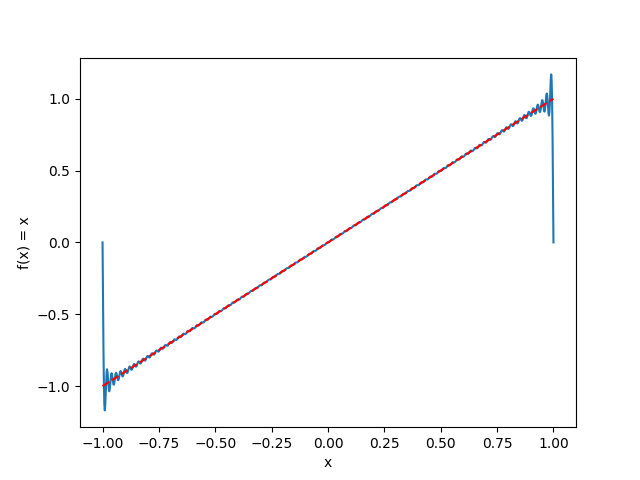
\includegraphics{Lab1/charts/Figure_1.png}

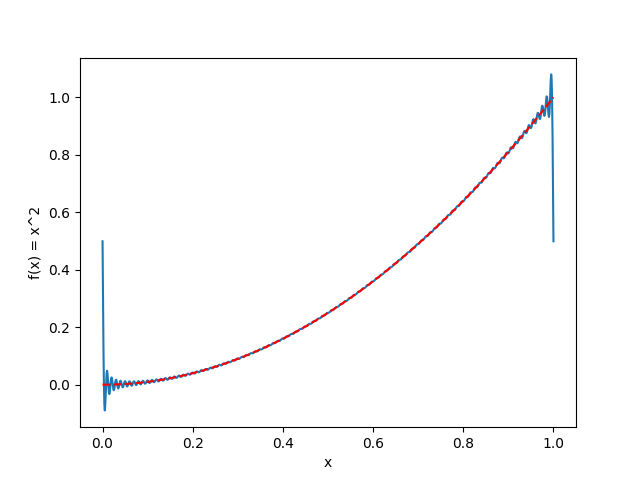
\includegraphics{Lab1/charts/Figure_2.png}
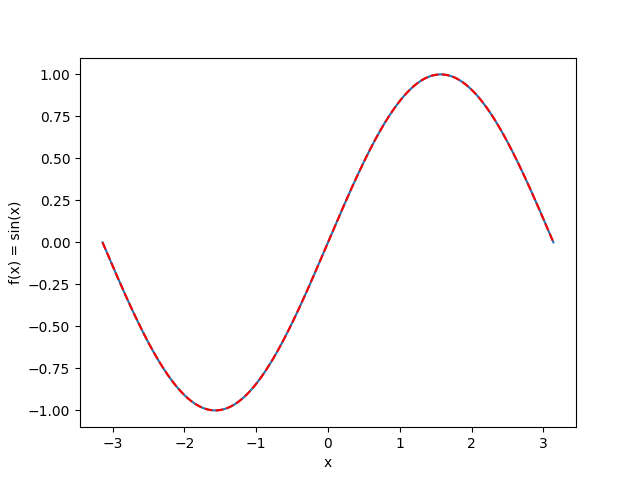
\includegraphics{Lab1/charts/Figure_3.png}

    
    \section{Schematy różnicowe}
\subsection{Definicja}

MRS opiera się na zastąpieniu pochodnych występująych w równaniach różniczkowych poprzez formuły zwane \textbf{schematami różnicowymi}. 

Aproksymacja pochodnej polega na rozwiązywaniu w efektywny sposób równań rózniczkowych zwyczajnych i cząstkowych, gdzie równania te dane są poprzez formuły zawierające nieznaną funkcję, którą chcemy wyznaczyć oraz pochodne dowolnych rzędów, a także stałe i znane funkcje.

Załóżmy, że funkcja $\textbf{f}$ jest różniczkowalna, co oznacza, że pochodna $f'(x_{0})$ jest zdefiniowana i ograniczona w pewnym otoczeniu punktu $x_{0}$.

Wprowadźmy trzy podstawowe schematy różnicowe w celu aproksymacji wartości pochodnej $f'(x_{0})$:

$\bullet$ Schemat \textit{w tył} (backward approximation scheme) 

$$f'(x_{0})\approx D_{-}f(x_{0})=\frac{f(x_{0})-f(x_{0}-h)}{h}$$

$\bullet$ Schemat \textit{w przód} (forward approximation scheme) 

$$f'(x_{0})\approx D_{+}f(x_{0})=\frac{f(x_{0}+h)-f(x_{0})}{h}$$

Obie formuły dają aproksymację rzędu pierwszego, co oznacza, że błąd jest proporcjonalny do wielkości h.

$\bullet$ Schemat \textit{centralny} (central approximation scheme) 

$$f'(x_{0})\approx D_{c}f(x_{0})=\frac{f(x_{0}+h)-f(x_{0}-h)}{2h} = \frac{1}{2}(D_{+}f(x_{0})+D_{-}f(x_{0}))$$

Schemat centralny jest rzędu drugiego, a więc $Error \sim h^{2}$.

	\subsection{Cel ćwiczenia}
Dla wybranej funkcji $f$ mieliśmy użyć schematów różnicowych w celu aproksymacji wartości jej pochodnej, pierwszej oraz drugiej.

Wybraliśmy funkcję $sinus$ w punkcie $x_{0} = 0.3$.

Następnie analitycznie obliczyliśmy pierwszą oraz drugą pochodną w obranym punkcie. Otrzymaliśmy:

$$sin'(0.3)=0.9553$$
$$sin''(0.3)=-0,2955$$

Następnie przystąpiliśmy do obliczeń numerycznych przy wykorzystaniu zaprezentowanych schematów różnicowych.
\newpage

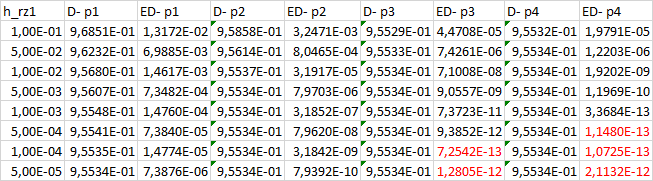
\includegraphics{Lab2/charts/rz1_log_Db_dane.png}

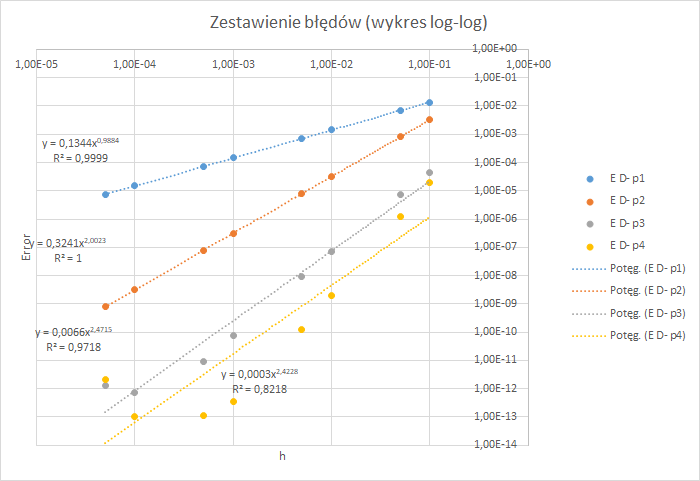
\includegraphics{Lab2/charts/rz1_log_Db.png} 
\newpage


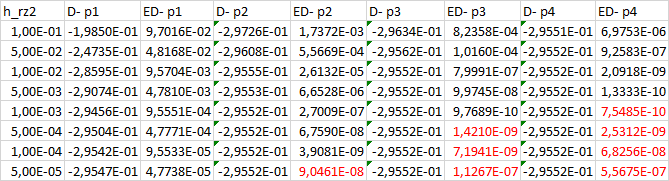
\includegraphics{Lab2/charts/rz2_log_Db_dane.png}

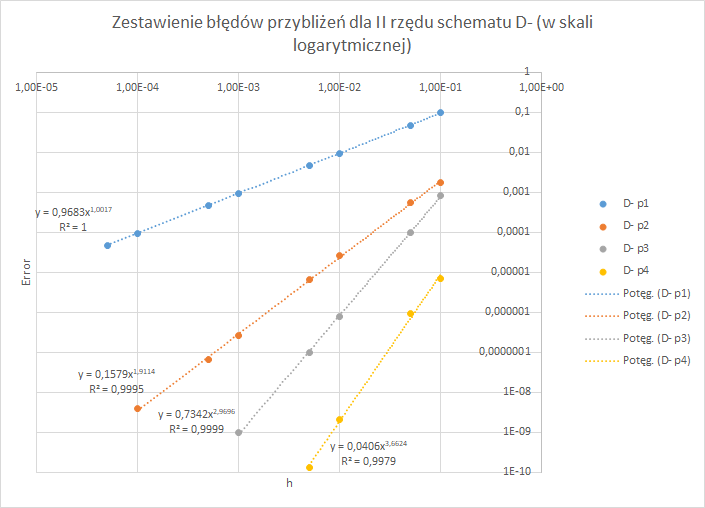
\includegraphics{Lab2/charts/rz2_log_Db.png}
\newpage


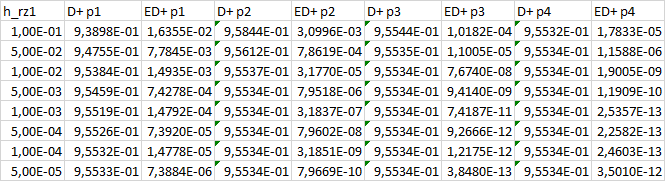
\includegraphics{Lab2/charts/rz1_log_Df_dane.png}

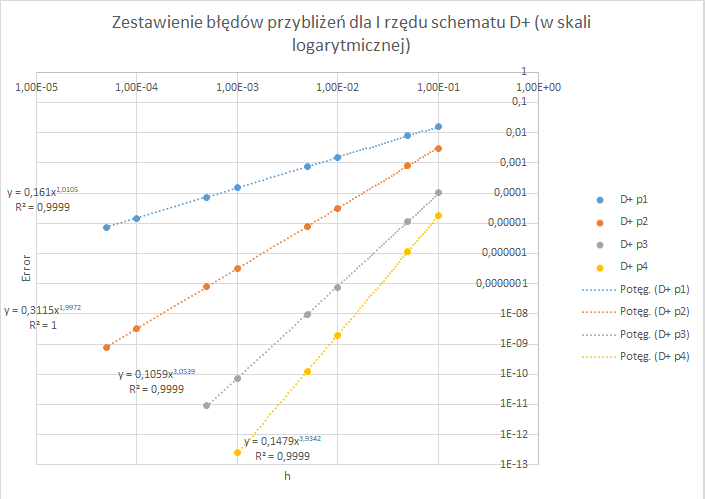
\includegraphics{Lab2/charts/rz1_log_Df.png}
\newpage


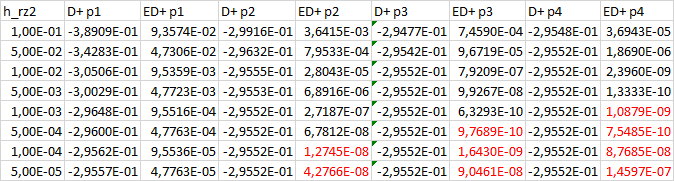
\includegraphics{Lab2/charts/rz2_log_Df_dane.png}

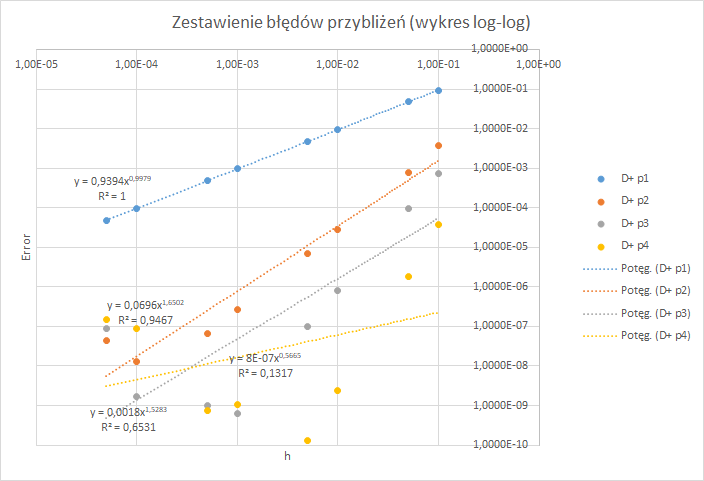
\includegraphics{Lab2/charts/rz2_log_Df.png}
\newpage


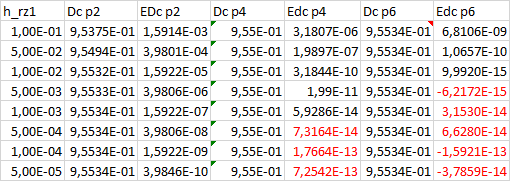
\includegraphics{Lab2/charts/rz1_log_Dc_dane.png}

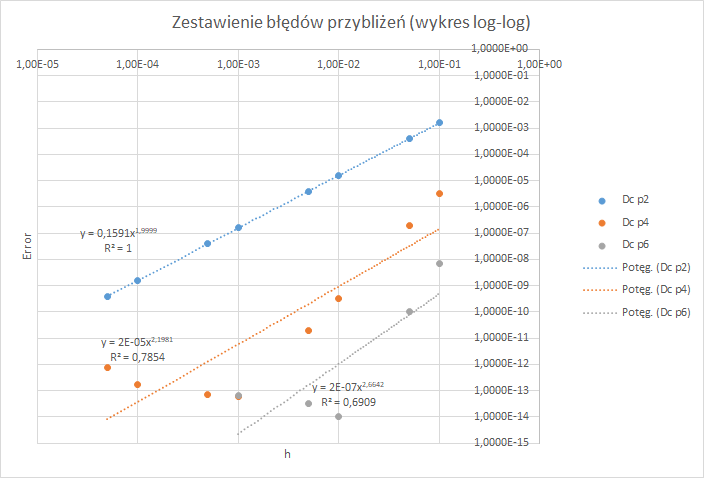
\includegraphics{Lab2/charts/rz1_log_Dc.png}
\newpage


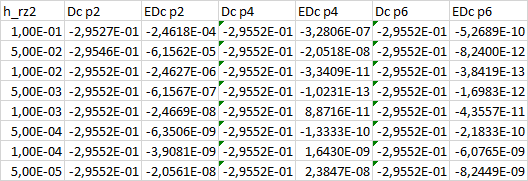
\includegraphics{Lab2/charts/rz2_log_Dc_dane.png}

Zestawienie błędów przybliżeń dla II rzędu schematu Dc na wykresie log-log nie jest możliwe. 

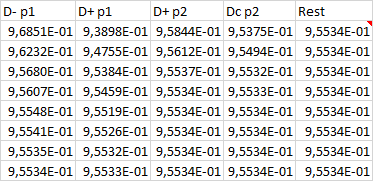
\includegraphics{Lab2/charts/rz1_log_e_dane.png}

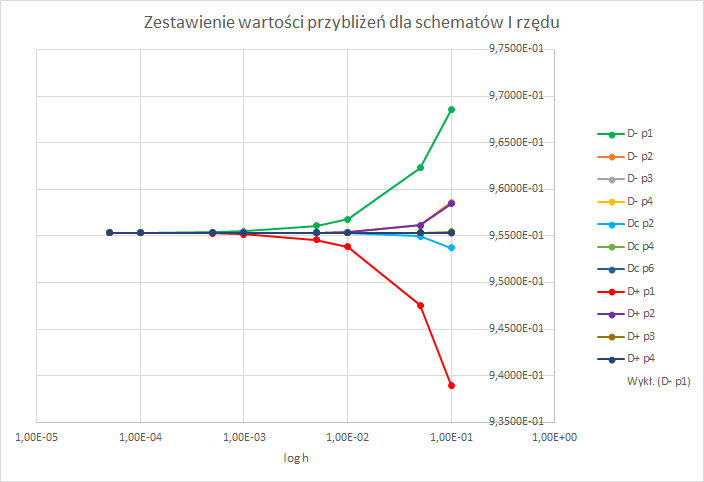
\includegraphics{Lab2/charts/rz1_log_e.png}
\newpage


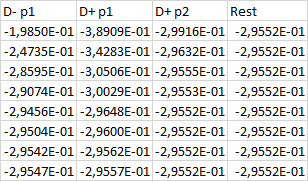
\includegraphics{Lab2/charts/rz2_log_e_dane.png}

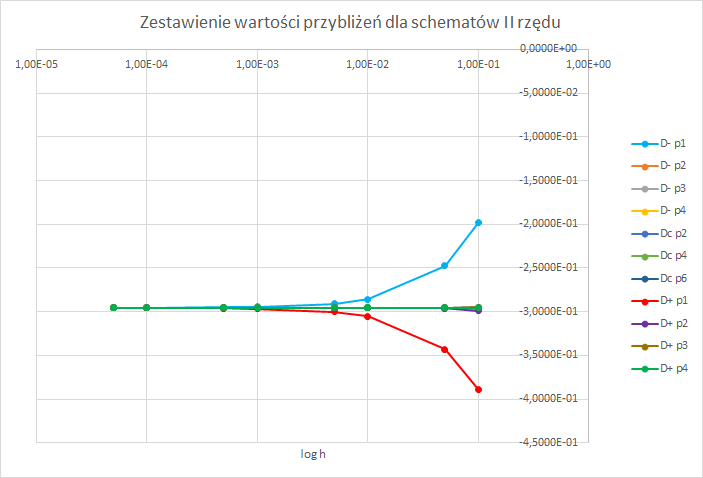
\includegraphics{Lab2/charts/rz2_log_e.png}
\newpage


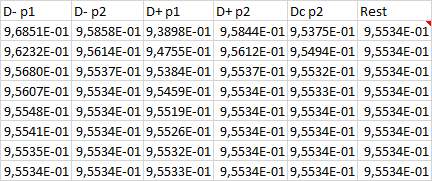
\includegraphics{Lab2/charts/rz1_e_dane.png}

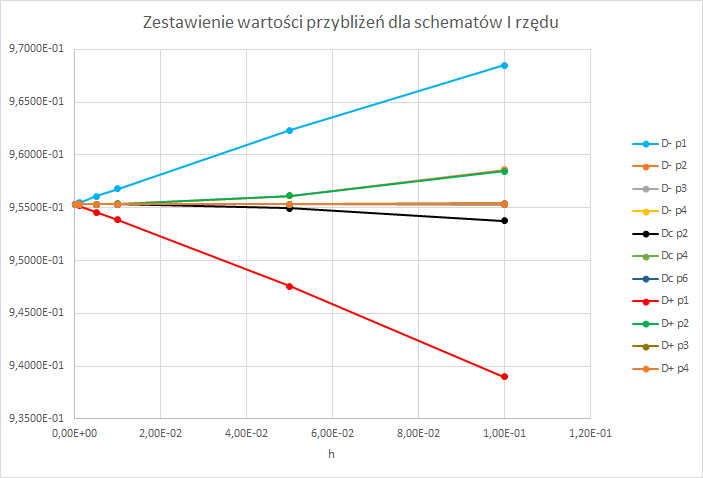
\includegraphics{Lab2/charts/rz1_e.png}
\newpage


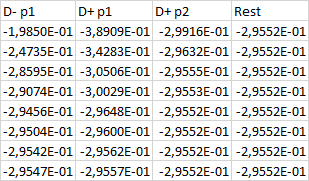
\includegraphics{Lab2/charts/rz2_e_dane.png}

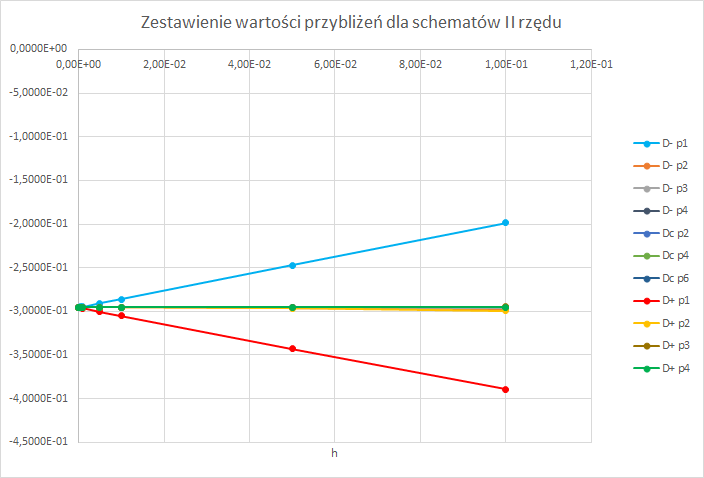
\includegraphics{Lab2/charts/rz2_e.png}




    
    \section{Zagadnienie brzegowe Dirichleta}
\subsection{Definicja}

Warunek brzegowy Dirichleta stosujemy w teorii równań różniczkowych zwyczajnych oraz cząstkowych (typu eliptycznego) II rzędu.

Polega ona na zalożeniu, że znane są wartości poszukiwanego rozwiązania na obu brzegach przedziału $[a,b]$, na którym określona jest funkcja będąca rozwiązaniem danego problemu.

Jeżeli dla równania różniczkowego (zwyczajnego lub cząstkowego) stawiamy warunek brzegowy Dirichleta (na całym brzegu), to mówimy o zagadnieniu (problemie) Dirichleta. 

\textbf{Warunek brzegowy Dirichleta (I rodzaju)}

\[
\begin{cases}
\vspace{0.1cm} 
\hspace{0,1cm}\alpha \cdot y'' + \beta \cdot y'+\gamma \cdot y=f \\
\vspace{0.1cm}
\hspace{0,1cm}y(a)=y_{a} \\
\hspace{0,1cm}y(b)=y_{b}
\end{cases}
\]
, gdzie:

$\alpha, \beta, \gamma, f$ są znanymi funkcjami
\newline
$y = y(x)$ jest poszukiwanym rozwiązaniem
\newline

\textbf{Zagadnienie Dirichleta}

Poszukujemy funckję $u$, której znane są wartości na brzegu. Taki problem da się rozwiązać analitycznie całkując dwukrotnie równanie.

\[
\begin{cases}
\vspace{0.1cm} 
\hspace{0,1cm}u''=f \\
\vspace{0.1cm}
\hspace{0,1cm}u|_{x=a}=u_{a} \\
\hspace{0,1cm}u|_{x=b}=u_{b}
\end{cases}
\]
\newline

My jednak sformułujemy to zagadnienie z użyciem MRS, otrzymamy wówczas aproksymację rozwiązania w wybranych przez nas węzłach.

Następnie porównamy metodę numeryczną oraz analityczną rozwiązania zadanego problemu.

\subsection{Cel ćwiczenia}

Naszym zadaniem było stworzenie algorytmu rozwiązującego następujące zagadnienia Dirichleta:

a)
\[
\begin{cases}
\vspace{0.1cm} 
\hspace{0,1cm}u''=-sin(x)-4\cdot sin(2x) \\
\vspace{0.1cm}
\hspace{0,1cm}u|_{x=0}=0 \\
\hspace{0,1cm}u|_{x=2\pi}=0
\end{cases}
\]
, gdzie:

$x\in [0,2\pi]$

Rozwiązanie analityczne: $\widetilde{u}(x) = sin(x) +sin(2x)$
\newpage
b)
\[
\begin{cases}
\vspace{0.1cm} 
\hspace{0,1cm}u''=12x \\
\vspace{0.1cm}
\hspace{0,1cm}u|_{x=0}=0 \\
\hspace{0,1cm}u|_{x=1}=1
\end{cases}
\]
, gdzie:

$x\in [0,1]$

Rozwiązanie analityczne: $\widetilde{u}(x) = 2x^{3}-x$

\vspace{0.3cm}
Ponadto zaprezentujemy wykres porównujący rozwiązanie numeryczne z rozwiązaniem analitycznym, a także wykres błędu $||E||_{\infty}$ w zależności od liczby obranych węzłów (n).

\subsection{Algorytm}
a)
\begin{samepage}
\begin{Shaded}
\begin{Highlighting}[]
\FunctionTok{clear}\NormalTok{, }\FunctionTok{clc}\NormalTok{;}
\CommentTok{#dane wejściowe}
\NormalTok{a=}\FloatTok{0}\NormalTok{;}
\NormalTok{b=}\FloatTok{2}\NormalTok{*}\BaseNTok{pi}\NormalTok{;}
\NormalTok{n = input('Podaj liczbe węzłów: ');}
\NormalTok{h = (b-a)/(n+}\FloatTok{1}\NormalTok{);}
\NormalTok{Ua = }\FloatTok{0}\NormalTok{;}
\NormalTok{Ub = }\FloatTok{0}\NormalTok{;}
\NormalTok{f = @(x) -}\FunctionTok{sin}\NormalTok{(x) - }\FloatTok{4}\NormalTok{*}\FunctionTok{sin}\NormalTok{(}\FloatTok{2}\NormalTok{*x);}
\NormalTok{g = @(x) }\FunctionTok{sin}\NormalTok{(x) + }\FunctionTok{sin}\NormalTok{(}\FloatTok{2}\NormalTok{*x);}
\CommentTok{#obliczenia}
\NormalTok{v1 = -}\FloatTok{2}\NormalTok{*}\FunctionTok{diag}\NormalTok{(}\FunctionTok{eye}\NormalTok{(n));}
\NormalTok{v2 = }\FunctionTok{diag}\NormalTok{(}\FunctionTok{eye}\NormalTok{(n-}\FloatTok{1}\NormalTok{));}
\NormalTok{A = }\FunctionTok{diag}\NormalTok{(v1) + }\FunctionTok{diag}\NormalTok{(v2,}\FloatTok{1}\NormalTok{) + }\FunctionTok{diag}\NormalTok{(v2,-}\FloatTok{1}\NormalTok{);}
\NormalTok{x= }\FunctionTok{linspace}\NormalTok{(a+h,b-h,n);}
\NormalTok{x2 = }\FunctionTok{linspace}\NormalTok{(a,b,n+}\FloatTok{2}\NormalTok{);}
\NormalTok{x3 = }\FunctionTok{linspace}\NormalTok{(a,b,100}\NormalTok{);}
\NormalTok{F = f(x)*h^}\FloatTok{2}\NormalTok{;}
\NormalTok{F(}\FloatTok{1}\NormalTok{) = F(}\FloatTok{1}\NormalTok{) - Ua;}
\NormalTok{F(n) = F(n) - Ub;}
\NormalTok{U = linsolve(A,F');}
\NormalTok{U = [Ua U' Ub];}
\CommentTok{#wykres}
\NormalTok{plot(x3, g(x3), x2, g(x2), 'ro');}
\NormalTok{legend('Metoda Analityczna','Metoda Numeryczna');}
\CommentTok{#error}
\NormalTok{E = max(abs(g(x2) - U));}
\end{Highlighting}
\end{Shaded}
\end{samepage}
\newpage
b)
\begin{samepage}
\begin{Shaded}
\begin{Highlighting}[]
\FunctionTok{clear}\NormalTok{, }\FunctionTok{clc}\NormalTok{;}
\CommentTok{#dane wejściowe}
\NormalTok{a=}\FloatTok{0}\NormalTok{;}
\NormalTok{b=}\FloatTok{1}\NormalTok{;}
\NormalTok{n = input('Podaj liczbe węzłów: ');}
\NormalTok{h = (b-a)/(n+}\FloatTok{1}\NormalTok{);}
\NormalTok{Ua = }\FloatTok{0}\NormalTok{;}
\NormalTok{Ub = }\FloatTok{1}\NormalTok{;}
\NormalTok{f = @(x) }\FloatTok{12}\NormalTok{*x;}
\NormalTok{g = @(x) }\FloatTok{2}\NormalTok{*x.^}\FloatTok{3}\NormalTok{-x;}
\CommentTok{#obliczenia}
\NormalTok{v1 = -}\FloatTok{2}\NormalTok{*}\FunctionTok{diag}\NormalTok{(}\FunctionTok{eye}\NormalTok{(n));}
\NormalTok{v2 = }\FunctionTok{diag}\NormalTok{(}\FunctionTok{eye}\NormalTok{(n-}\FloatTok{1}\NormalTok{));}
\NormalTok{A = }\FunctionTok{diag}\NormalTok{(v1) + }\FunctionTok{diag}\NormalTok{(v2,}\FloatTok{1}\NormalTok{) + }\FunctionTok{diag}\NormalTok{(v2,-}\FloatTok{1}\NormalTok{);}
\NormalTok{x= }\FunctionTok{linspace}\NormalTok{(a+h,b-h,n);}
\NormalTok{x2 = }\FunctionTok{linspace}\NormalTok{(a,b,n+}\FloatTok{2}\NormalTok{);}
\NormalTok{x3 = }\FunctionTok{linspace}\NormalTok{(a,b,100}\NormalTok{);}
\NormalTok{F = f(x)*h^}\FloatTok{2}\NormalTok{;}
\NormalTok{F(}\FloatTok{1}\NormalTok{) = F(}\FloatTok{1}\NormalTok{) - Ua;}
\NormalTok{F(n) = F(n) - Ub;}
\NormalTok{U = linsolve(A,F');}
\NormalTok{U = [Ua U' Ub];}
\CommentTok{#wykres}
\NormalTok{plot(x3, g(x3), x2, g(x2), 'ro');}
\NormalTok{legend('Metoda Analityczna','Metoda Numeryczna',0);}
\CommentTok{#error}
\NormalTok{E = max(abs(g(x2) - U));}

\end{Highlighting}
\end{Shaded}
\end{samepage}
\newpage
\subsection{Wykresy}
a)

Dla 10 węzłów:

\begin{figure}[!ht]
	\begin{center}
		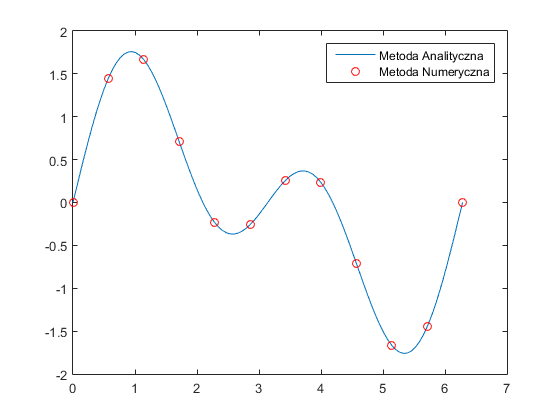
\includegraphics[width=0.8\textwidth]{Lab3/charts/zad1/10.png}
	\end{center}
\end{figure}

Dla 25 węzłów:

\begin{figure}[!ht]
	\begin{center}
		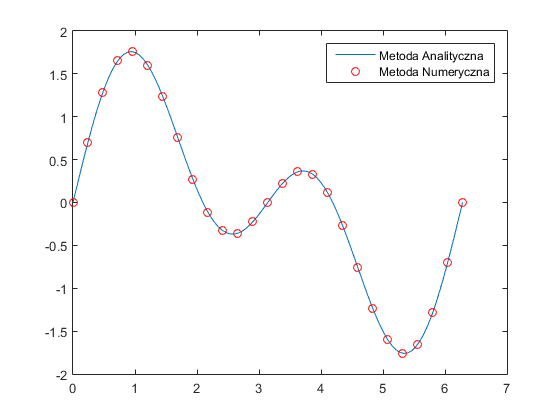
\includegraphics[width=0.8\textwidth]{Lab3/charts/zad1/25.png}
	\end{center}
\end{figure}

\newpage

Dla 100 węzłów:
	

\begin{figure}[!ht]
	\begin{center}
		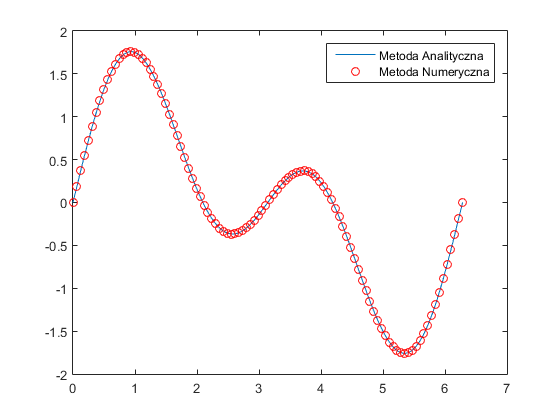
\includegraphics[width=0.8\textwidth]{Lab3/charts/zad1/100.png}
	\end{center}
\end{figure}



Dla 1000 węzłów:

\begin{figure}[!ht]
	\begin{center}
		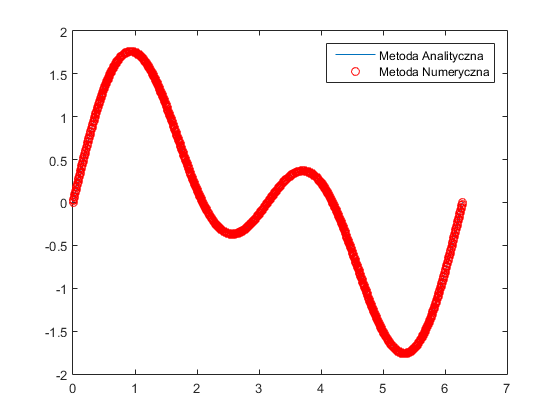
\includegraphics[width=0.8\textwidth]{Lab3/charts/zad1/1000.png}
	\end{center}
\end{figure}

\newpage

Błąd metody w zależności od liczby węzłów:

\begin{figure}[!ht]
	\begin{center}
		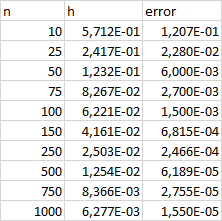
\includegraphics[width=0.8\textwidth]{Lab3/charts/zad1/error_dane.png}
	\end{center}
\end{figure}

\begin{figure}[!ht]
	\begin{center}
		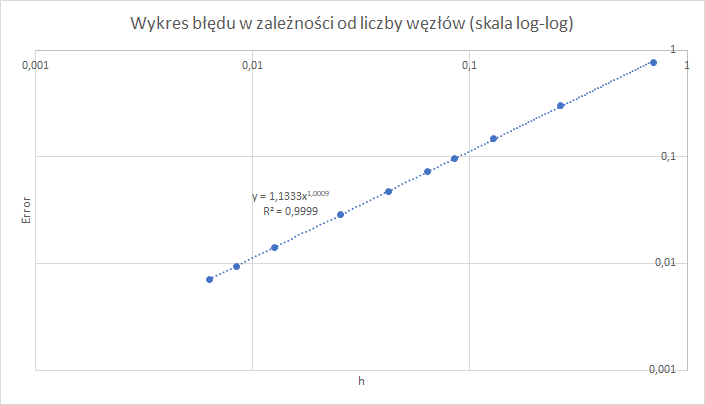
\includegraphics[width=0.8\textwidth]{Lab3/charts/zad1/error.png}
	\end{center}
\end{figure}

\newpage

b)

Dla 10 węzłów:

\begin{figure}[!ht]
	\begin{center}
		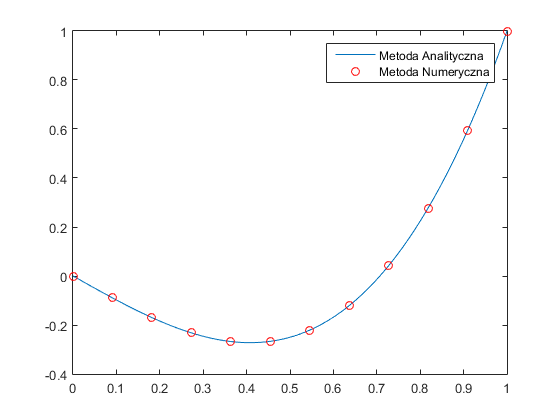
\includegraphics[width=0.8\textwidth]{Lab3/charts/zad2/10.png}
	\end{center}
\end{figure}

Dla 25 węzłów:

\begin{figure}[!ht]
	\begin{center}
		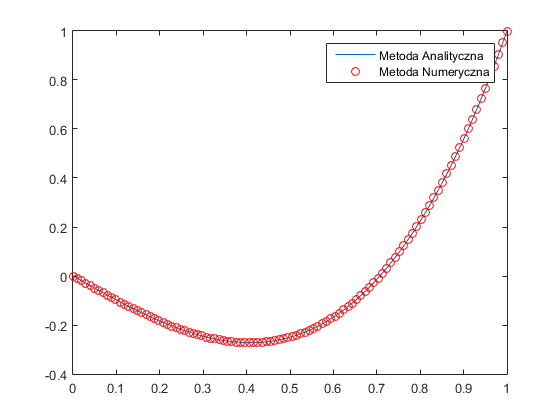
\includegraphics[width=0.8\textwidth]{Lab3/charts/zad2/25.png}
	\end{center}
\end{figure}

\newpage

Dla 100 węzłów:

\begin{figure}[!ht]
	\begin{center}
		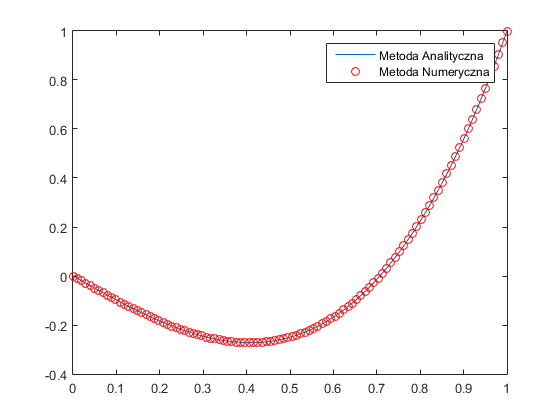
\includegraphics[width=0.8\textwidth]{Lab3/charts/zad2/100.png}
	\end{center}
\end{figure}

Dla 1000 węzłów:

\begin{figure}[!ht]
	\begin{center}
		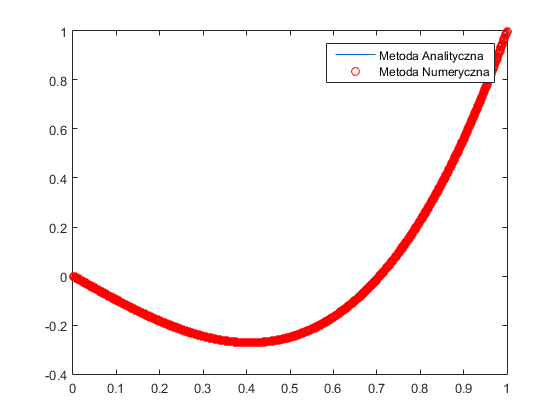
\includegraphics[width=0.8\textwidth]{Lab3/charts/zad2/1000.png}
	\end{center}
\end{figure}

\newpage

Błąd metody w zależności od liczby węzłów:

\begin{figure}[!ht]
	\begin{center}
		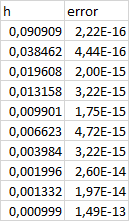
\includegraphics[width=0.8\textwidth]{Lab3/charts/zad2/error_dane.png}
	\end{center}
\end{figure}

\begin{figure}[!ht]
	\begin{center}
		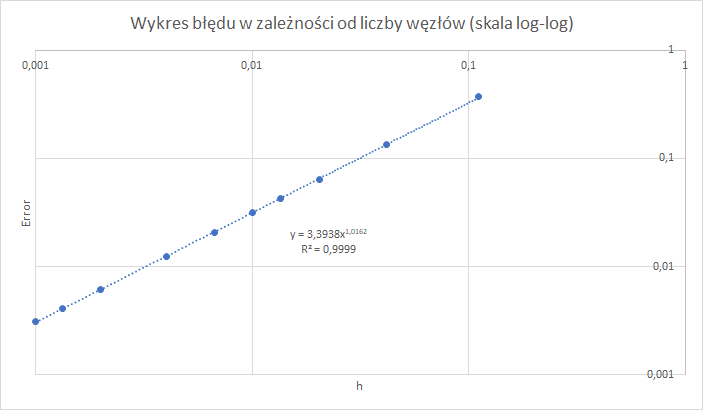
\includegraphics[width=0.8\textwidth]{Lab3/charts/zad2/error.png}
	\end{center}
\end{figure}


    
    \section{Ogólne zagadnienia brzegowe II rzędu}
\subsection{Warunki brzegowe typu Dirichletta}

Rozważając najbardziej ogólne zagadnienie brzegowe rzędu II z warunkami brzegowymi typu Dirichletta postaci:

\[
\begin{cases}
\vspace{0.1cm} 
\hspace{0,1cm} a(x) u'' + b(x)u' + c(x)u =f(x) \\
\vspace{0.1cm}
\hspace{0,1cm}u|_{x=a} = u_{a} \\
\hspace{0,1cm}u|_{x=b} = u_{b}
\end{cases}
\]
, gdzie:
$x\in[a,b]$

$a(x), b(x), c(x), f(x)$ są znanymi funkcjami
\newline
$u = u(x)$ jest poszukiwanym rozwiązaniem
\newline

Stosowanie schematów na pochodną różnego rzędu (I oraz II) o tej samej dokładności skutkuje tym, że cała metoda jest rzędu II.

\subsection{Cel ćwiczenia}
Na laboratorium otrzymaliśmy następujące równania dla których mieliśmy stworzyć rozwiązujący je algorytm.

a)
\[
\begin{cases}
\vspace{0.1cm} 
\hspace{0,1cm} u'' - 4u =-4x \\
\vspace{0.1cm}
\hspace{0,1cm}u|_{x=0} = 0 \\
\hspace{0,1cm}u|_{x=1} = 2
\end{cases}
\]
, gdzie:
$x\in[0,1]$
\\
Rozwiązanie analityczne: $\widetilde{u}(x) = e^2(e^4-1)^{-1} (e^{2x} - e^{-2x}) + x$
\\
\\
b)
\[
\begin{cases}
\vspace{0.1cm} 
\hspace{0,1cm} u'' -u'- 2u =cos(x) \\
\vspace{0.1cm}
\hspace{0,1cm}u|_{x=0} = -\dfrac{3}{10} \\
\hspace{0,1cm}u|_{x=\dfrac{\pi}{2}} = -\dfrac{1}{10}
\end{cases}
\]
, gdzie:
$x\in[0, \dfrac{\pi}{2}]$
\\
Rozwiązanie analityczne: $\widetilde{u}(x) = -\dfrac{1}{10}(sin(x) + 3cos(x))$
\\
\\
c)
\[
\begin{cases}
\vspace{0.1cm} 
\hspace{0,1cm} -x^2u'' +2xu' +2u=-4x^2 \\
\vspace{0.1cm}
\hspace{0,1cm}u|_{x=0} = 0 \\
\hspace{0,1cm}u|_{x=1} = 0
\end{cases}
\]
, gdzie:
$x\in[0,1]$
\\
Rozwiązanie analityczne: $\widetilde{u}(x) = x^2 - x$

\vspace{0.3cm}
Ponadto zaprezentujemy wykres porównujący rozwiązanie numeryczne z rozwiązaniem analitycznym, a także wykres błędu $||E||_{\infty}$ w zależności od liczby obranych węzłów (n).
%\begin{samepage}
\newpage
\subsection{Rozwiązanie}
%\textbf{Warunek brzegowy Dirichleta (I rodzaju)}
Poniżej przedstawiony został algorytm rozwiązania powyższych równań z przykładowymi danymi wejściowymi z podpunktu a).


\begin{samepage}
    \begin{Shaded}
\begin{Highlighting}[]
\FunctionTok{clear}\NormalTok{, }\FunctionTok{clc}\NormalTok{;}
\CommentTok{# Dane wejściowe}
\NormalTok{f = @(x) -}\FloatTok{4}\NormalTok{*x;}
\NormalTok{g = @(x) }\FunctionTok{exp}\NormalTok{(}\FloatTok{2}\NormalTok{) * (}\FunctionTok{exp}\NormalTok{(}\FloatTok{4}\NormalTok{) - }\FloatTok{1} \NormalTok{)^-}\FloatTok{1} \NormalTok{* (}\FunctionTok{exp}\NormalTok{(}\FloatTok{2}\NormalTok{*x) - }\FunctionTok{exp}\NormalTok{(-}\FloatTok{2}\NormalTok{*x)) + x;}
\NormalTok{a = }\FloatTok{0}\NormalTok{;}
\NormalTok{b = }\FloatTok{1}\NormalTok{;}
\NormalTok{ax = @(x) }\FloatTok{1}\NormalTok{;}
\NormalTok{bx = @(x) }\FloatTok{0}\NormalTok{;}
\NormalTok{cx = @(x) -}\FloatTok{4}\NormalTok{;}
\NormalTok{ua = }\FloatTok{0}\NormalTok{;}
\NormalTok{ub = }\FloatTok{2}\NormalTok{;}
\NormalTok{c = b-a;}
\NormalTok{n = }\FloatTok{10}\NormalTok{;}
\NormalTok{h = c/(n+}\FloatTok{1}\NormalTok{);}
\NormalTok{x = }\FunctionTok{linspace}\NormalTok{((a+h),(b-h),n);}
\CommentTok{# Obliczenia}
\NormalTok{a1 = (-}\FloatTok{2} \NormalTok{.* ax(x) + cx(x) .*h^}\FloatTok{2}\NormalTok{)' .* }\FunctionTok{diag}\NormalTok{(}\FunctionTok{eye}\NormalTok{(n));}
\NormalTok{A1 = }\FunctionTok{diag}\NormalTok{(a1);}
\NormalTok{a2 = (ax(x(}\FloatTok{2}\NormalTok{:n)) -}\FloatTok{1}\NormalTok{/}\FloatTok{2} \NormalTok{.* bx(x(}\FloatTok{2}\NormalTok{:n)) .*h)' .* }\FunctionTok{diag}\NormalTok{(}\FunctionTok{eye}\NormalTok{(n-}\FloatTok{1}\NormalTok{));}
\NormalTok{A2 = }\FunctionTok{diag}\NormalTok{(a2, -}\FloatTok{1}\NormalTok{);}
\NormalTok{a3 = (ax(x(}\FloatTok{1}\NormalTok{:n-}\FloatTok{1}\NormalTok{)) +}\FloatTok{1}\NormalTok{/}\FloatTok{2} \NormalTok{.* bx(x(}\FloatTok{1}\NormalTok{:n-}\FloatTok{1}\NormalTok{)) .*h)' .* }\FunctionTok{diag}\NormalTok{(}\FunctionTok{eye}\NormalTok{(n-}\FloatTok{1}\NormalTok{));}
\NormalTok{A3 = }\FunctionTok{diag}\NormalTok{(a3, }\FloatTok{1}\NormalTok{);}
\NormalTok{A = A1  + A2 + A3;}
\NormalTok{F = (h^}\FloatTok{2} \NormalTok{* f(x));}
\NormalTok{F(}\FloatTok{1}\NormalTok{) = F(}\FloatTok{1}\NormalTok{) - ua * (ax(}\FloatTok{1}\NormalTok{) - }\FloatTok{1}\NormalTok{/}\FloatTok{2} \NormalTok{* bx(}\FloatTok{1}\NormalTok{)*h);}
\NormalTok{F(n) = F(n) - ub * (ax(n) + }\FloatTok{1}\NormalTok{/}\FloatTok{2} \NormalTok{* bx(n)*h);}
\NormalTok{U = linsolve(A,F');}
\NormalTok{U = [ua U' ub];}
\NormalTok{X = [a x b];}
\CommentTok{# Wykres}
\FunctionTok{plot}\NormalTok{(X, U, X, g(X), }\StringTok{'ro'}\NormalTok{);}
\CommentTok{# Błąd}
\NormalTok{E = }\FunctionTok{max}\NormalTok{(}\FunctionTok{abs}\NormalTok{(g(X) - U));}
\end{Highlighting}
\end{Shaded}


\end{samepage}

\newpage
\subsection{Wykresy}

a)\\
\begin{samepage}
Dla 10 węzłów:

%{\centering
    
 %   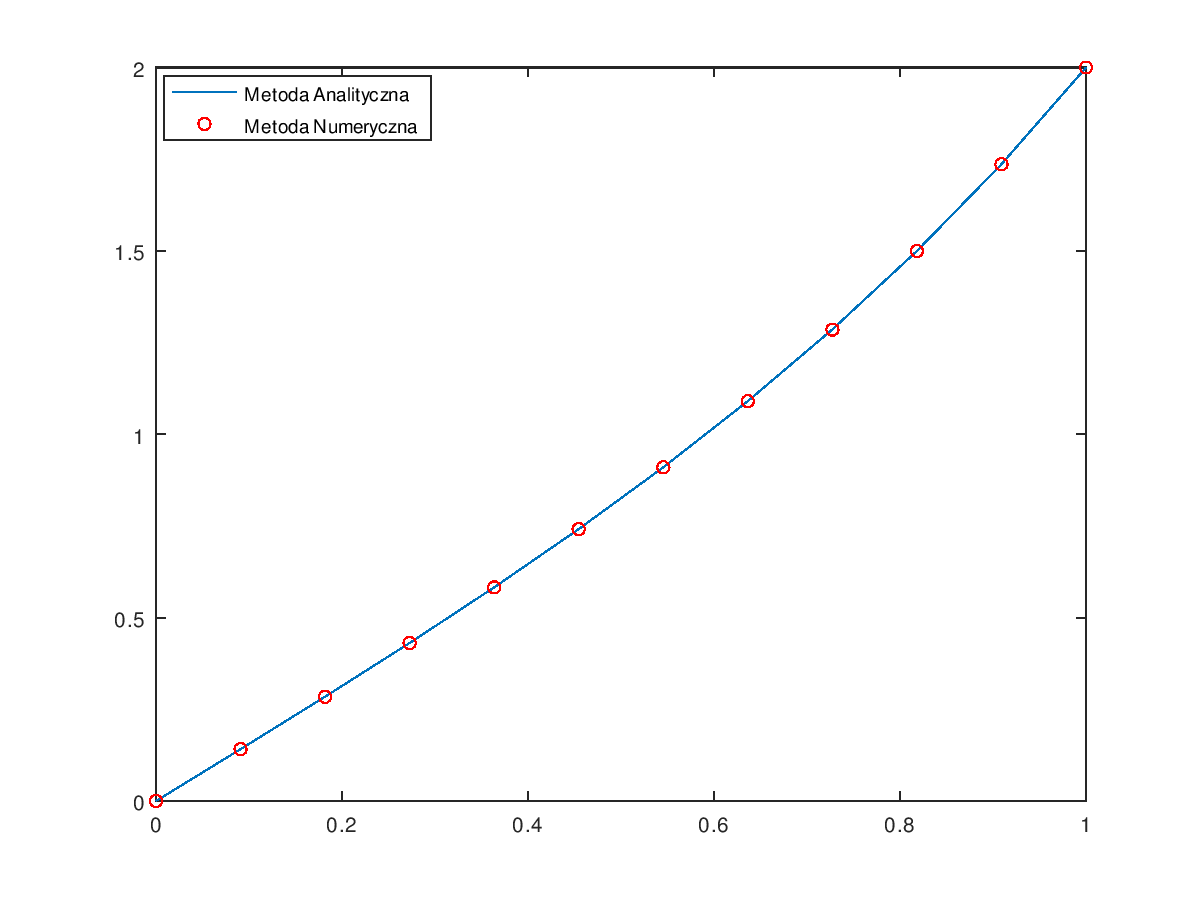
\includegraphics{Lab4/charts/zad1/zad1_n_10.png}
    
%}
\FloatBarrier
\begin{figure}[!ht]
    \begin{center}
        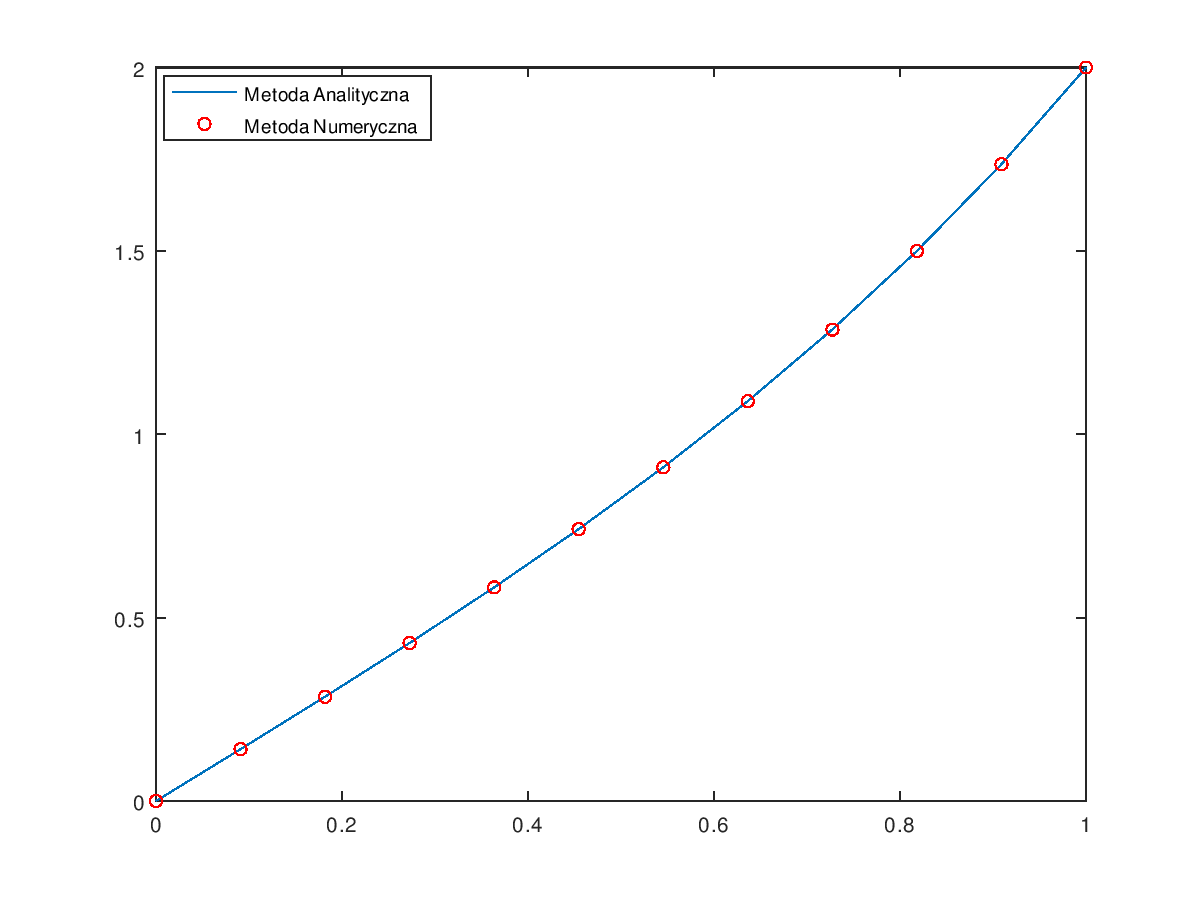
\includegraphics[width=0.8\textwidth]{Lab4/charts/zad1/zad1_n_10.png}
    \end{center}
    %\caption{Schemat logiczny w edytorze LAD oraz tabela symboli}
    %\label{fig:picture}
\end{figure}
\FloatBarrier
\end{samepage}

\begin{samepage}
Dla 25 węzłów:
\begin{figure}[!ht]
    \begin{center}
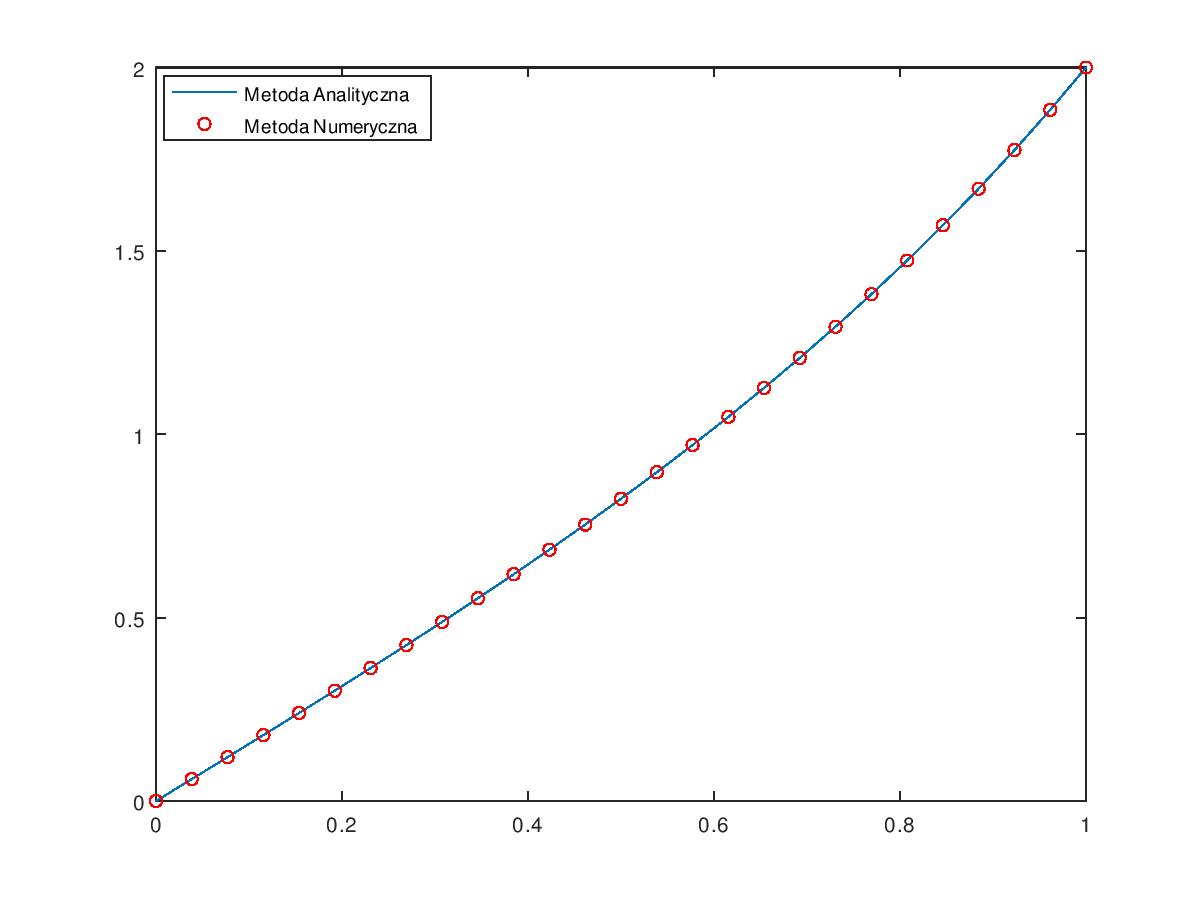
\includegraphics[width=0.8\textwidth]{Lab4/charts/zad1/zad1_n_25.png}
    \end{center}
    %\caption{Schemat logiczny w edytorze LAD oraz tabela symboli}
    %\label{fig:picture}
\end{figure}
\FloatBarrier
\end{samepage}

\newpage
\begin{samepage}
    
Dla 100 węzłów:
\begin{figure}[!ht]
    \begin{center}
    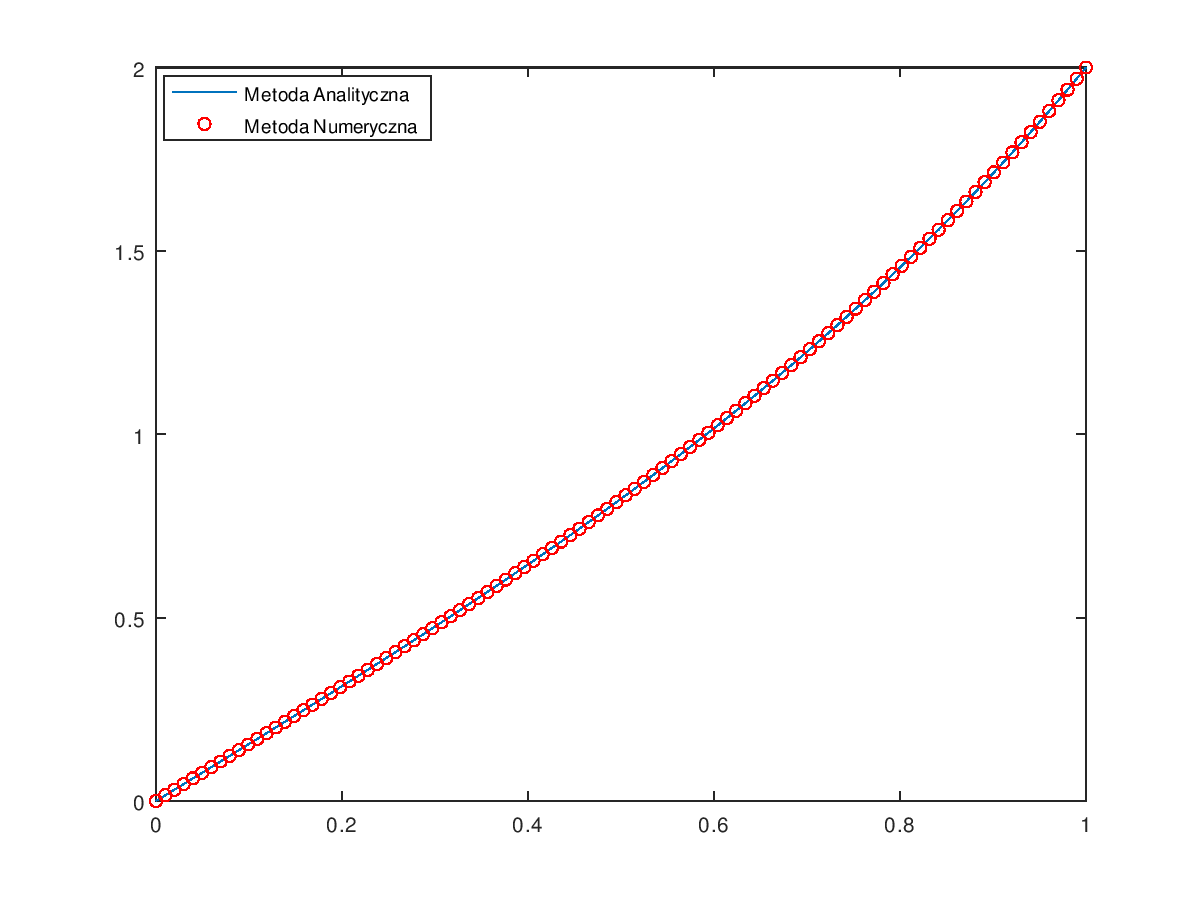
\includegraphics[width=0.8\textwidth]{Lab4/charts/zad1/zad1_n_100.png}
    \end{center}
    %\caption{Schemat logiczny w edytorze LAD oraz tabela symboli}
    %\label{fig:picture}
\end{figure}
\FloatBarrier
\end{samepage}
    
\begin{samepage}
Dla 1000 węzłów:

\begin{figure}[!ht]
    \begin{center}
    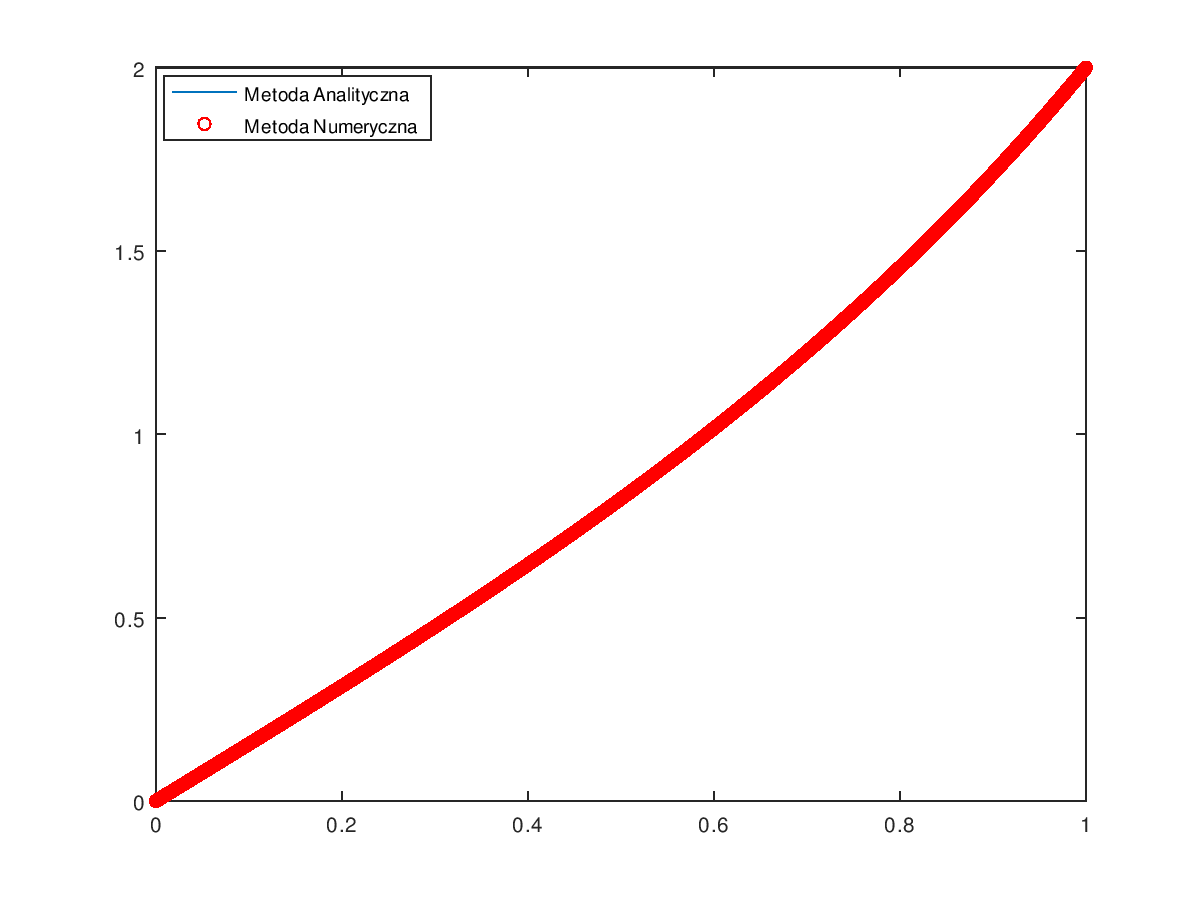
\includegraphics[width=0.8\textwidth]{Lab4/charts/zad1/zad1_n_1000.png}
    \end{center}
    %\caption{Schemat logiczny w edytorze LAD oraz tabela symboli}
    %\label{fig:picture}
\end{figure}
\FloatBarrier
\end{samepage}    

\newpage

\begin{samepage}
Błąd metody w zależności od liczby węzłów:
    \begin{figure}[!ht]
        \begin{center}
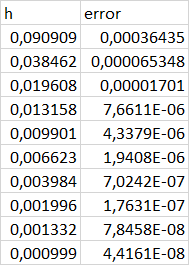
\includegraphics[width=0.8\textwidth]{Lab4/charts/zad1/error_dane.png}
        \end{center}
        %\caption{Schemat logiczny w edytorze LAD oraz tabela symboli}
        %\label{fig:picture}
    \end{figure}
    \FloatBarrier
\end{samepage} 

\begin{samepage}
    
    \begin{figure}[!ht]
        \begin{center}
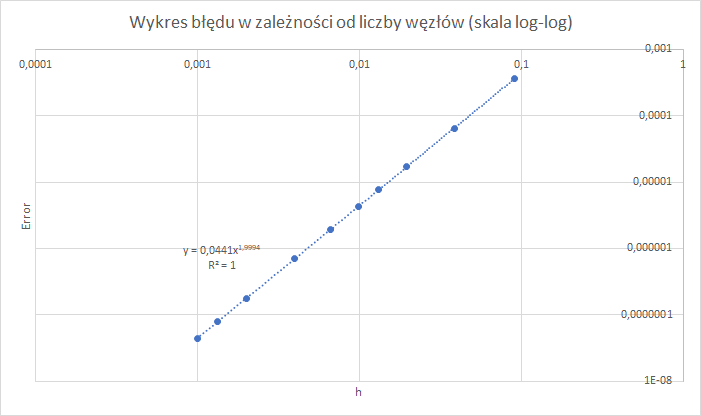
\includegraphics[width=0.8\textwidth]{Lab4/charts/zad1/error.png}
        \end{center}
        %\caption{Schemat logiczny w edytorze LAD oraz tabela symboli}
        %\label{fig:picture}
    \end{figure}
    \FloatBarrier
\end{samepage} 


\newpage
b)\\
\begin{samepage}
    Dla 10 węzłów:
    
    %{\centering
    
    %   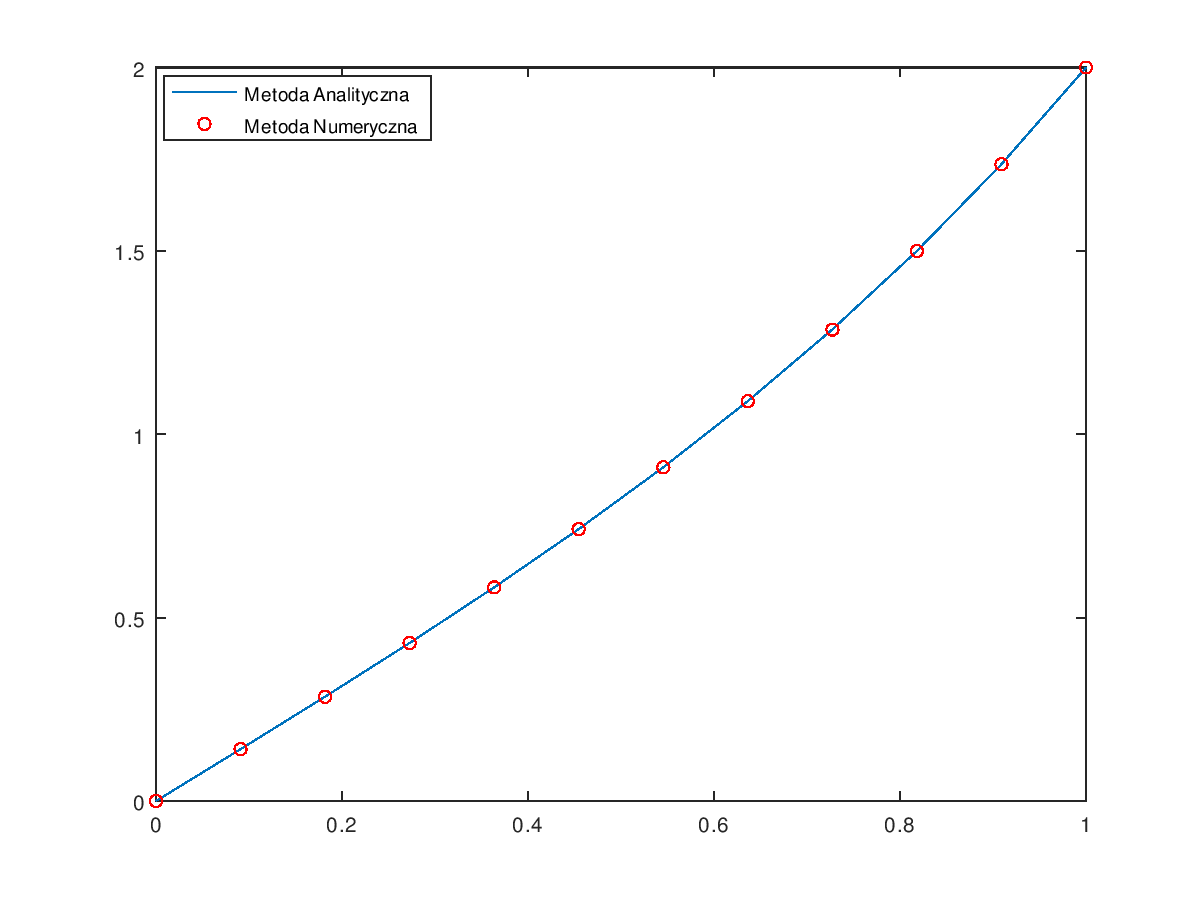
\includegraphics{Lab4/charts/zad1/zad1_n_10.png}
    
    %}
    \FloatBarrier
    \begin{figure}[!ht]
        \begin{center}
            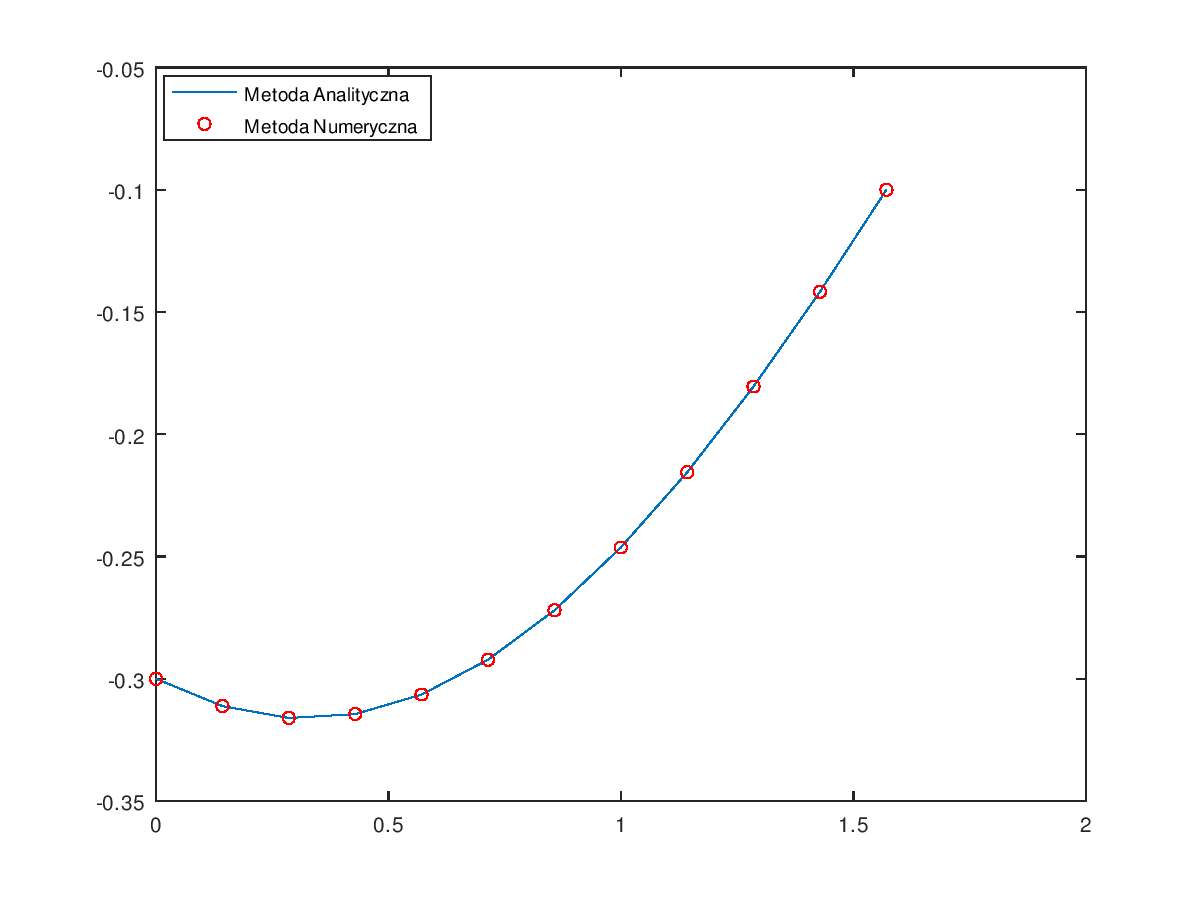
\includegraphics[width=0.8\textwidth]{Lab4/charts/zad2/zad2_n_10.png}
        \end{center}
        %\caption{Schemat logiczny w edytorze LAD oraz tabela symboli}
        %\label{fig:picture}
    \end{figure}
    \FloatBarrier
\end{samepage}

\begin{samepage}
    Dla 25 węzłów:
    \begin{figure}[!ht]
        \begin{center}
            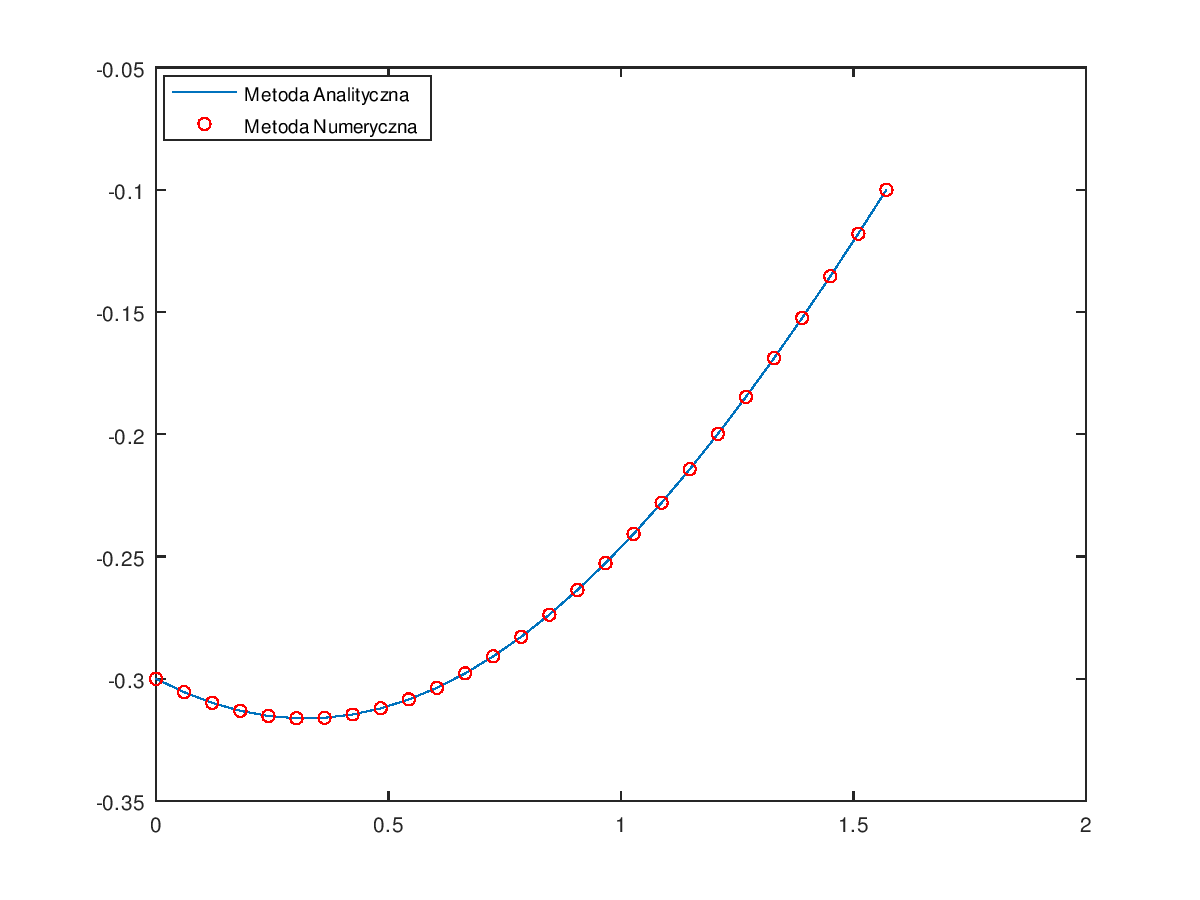
\includegraphics[width=0.8\textwidth]{Lab4/charts/zad2/zad2_n_25.png}
        \end{center}
        %\caption{Schemat logiczny w edytorze LAD oraz tabela symboli}
        %\label{fig:picture}
    \end{figure}
    \FloatBarrier
\end{samepage}

\newpage
\begin{samepage}
    
    Dla 100 węzłów:
    \begin{figure}[!ht]
        \begin{center}
            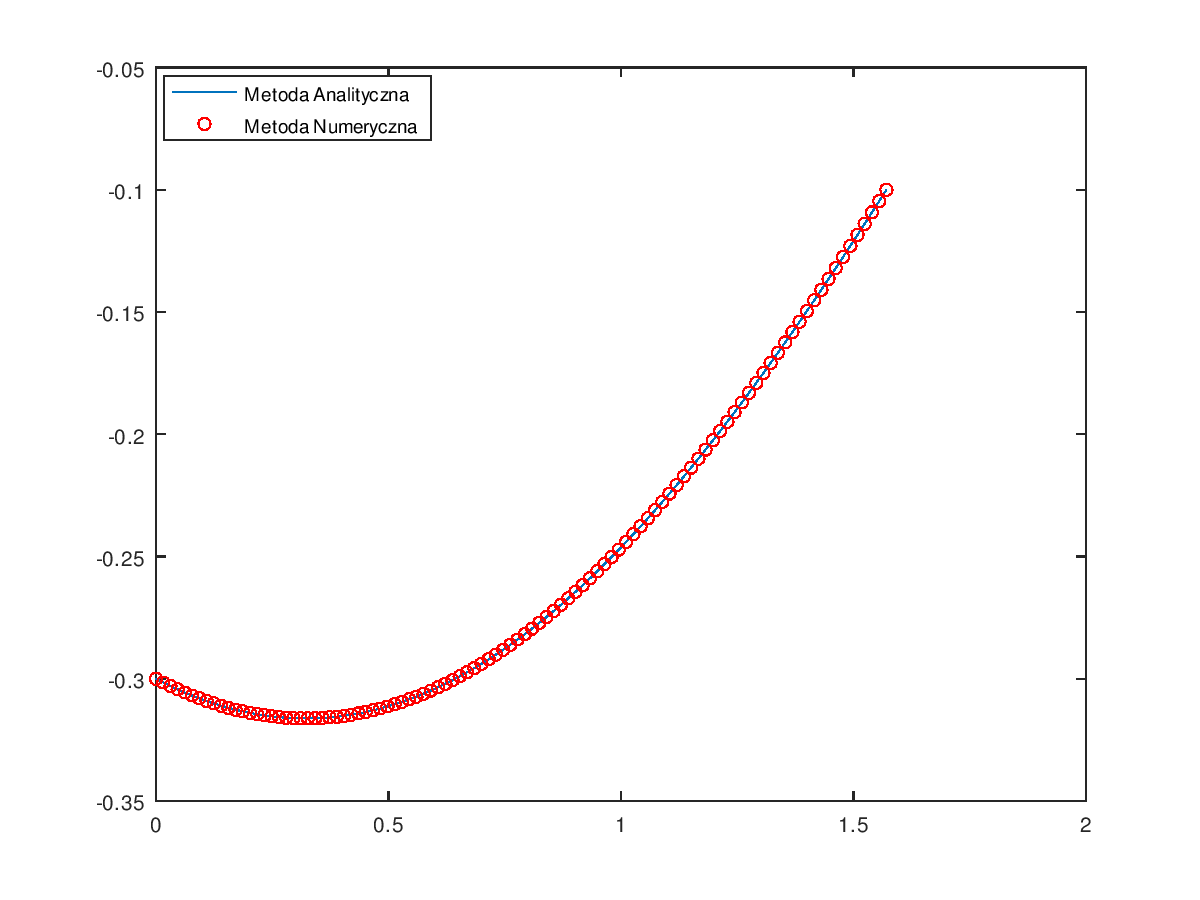
\includegraphics[width=0.8\textwidth]{Lab4/charts/zad2/zad2_n_100.png}
        \end{center}
        %\caption{Schemat logiczny w edytorze LAD oraz tabela symboli}
        %\label{fig:picture}
    \end{figure}
    \FloatBarrier
\end{samepage}


\begin{samepage}
    Dla 1000 węzłów:
    
    \begin{figure}[!ht]
        \begin{center}
            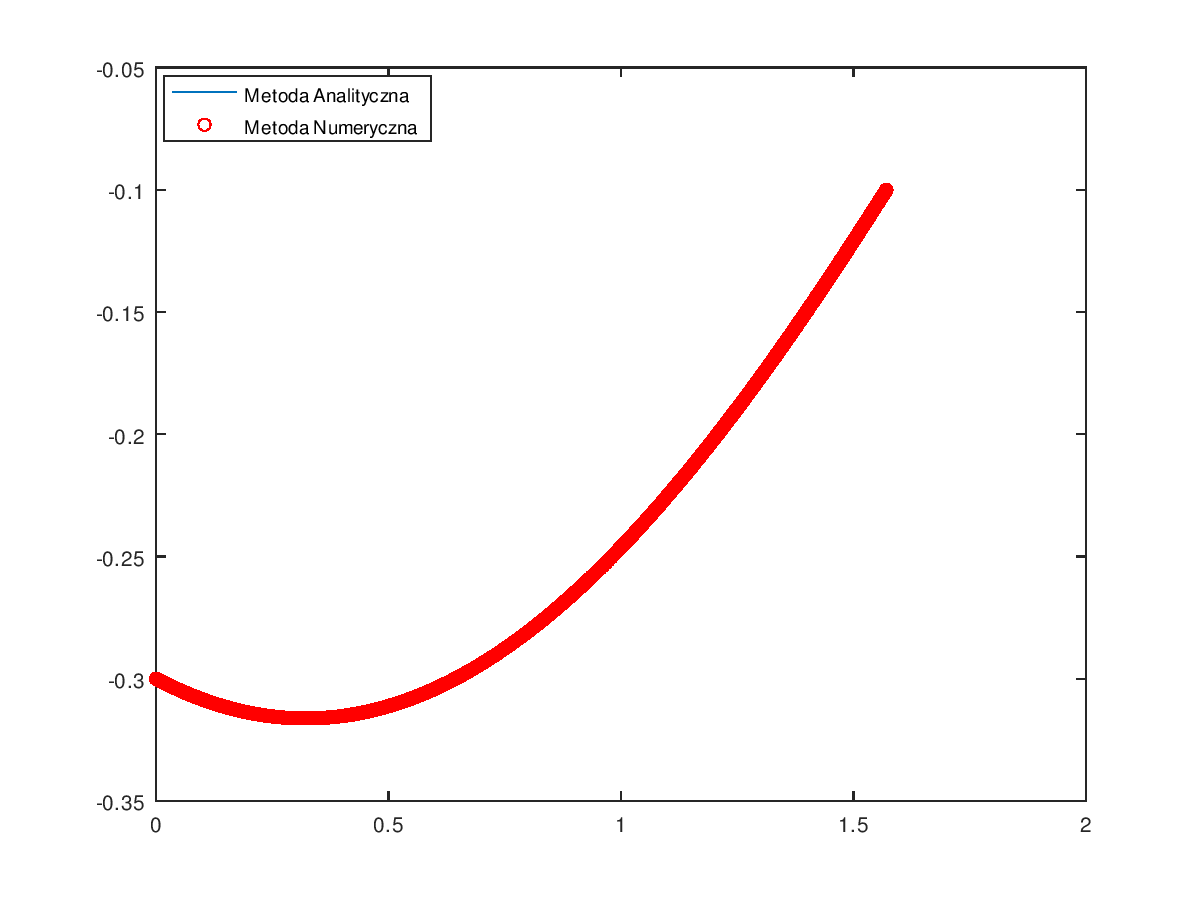
\includegraphics[width=0.8\textwidth]{Lab4/charts/zad2/zad2_n_1000.png}
        \end{center}
        %\caption{Schemat logiczny w edytorze LAD oraz tabela symboli}
        %\label{fig:picture}
    \end{figure}
    \FloatBarrier
\end{samepage}    

\newpage

\begin{samepage}
    Błąd metody w zależności od liczby węzłów:
    \begin{figure}[!ht]
        \begin{center}
            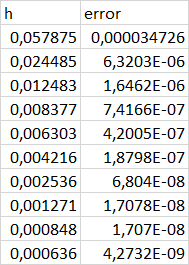
\includegraphics[width=0.8\textwidth]{Lab4/charts/zad2/error_dane.png}
        \end{center}
        %\caption{Schemat logiczny w edytorze LAD oraz tabela symboli}
        %\label{fig:picture}
    \end{figure}
    \FloatBarrier
\end{samepage} 

\begin{samepage}
    
    \begin{figure}[!ht]
        \begin{center}
            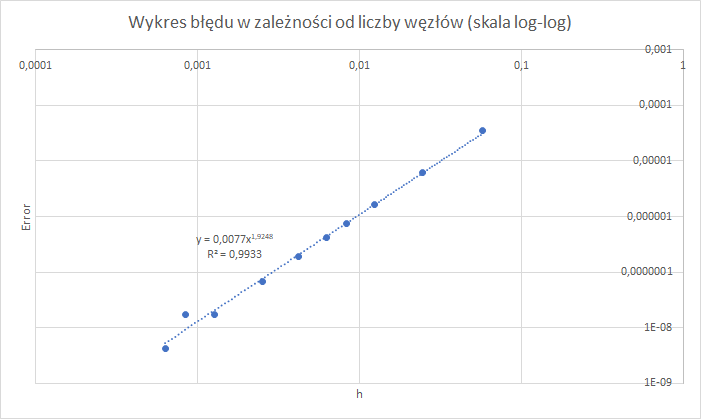
\includegraphics[width=0.8\textwidth]{Lab4/charts/zad2/error.png}
        \end{center}
        %\caption{Schemat logiczny w edytorze LAD oraz tabela symboli}
        %\label{fig:picture}
    \end{figure}
    \FloatBarrier
\end{samepage}   

\newpage
c)\\
\begin{samepage}
    Dla 10 węzłów:
    
    %{\centering
    
    %   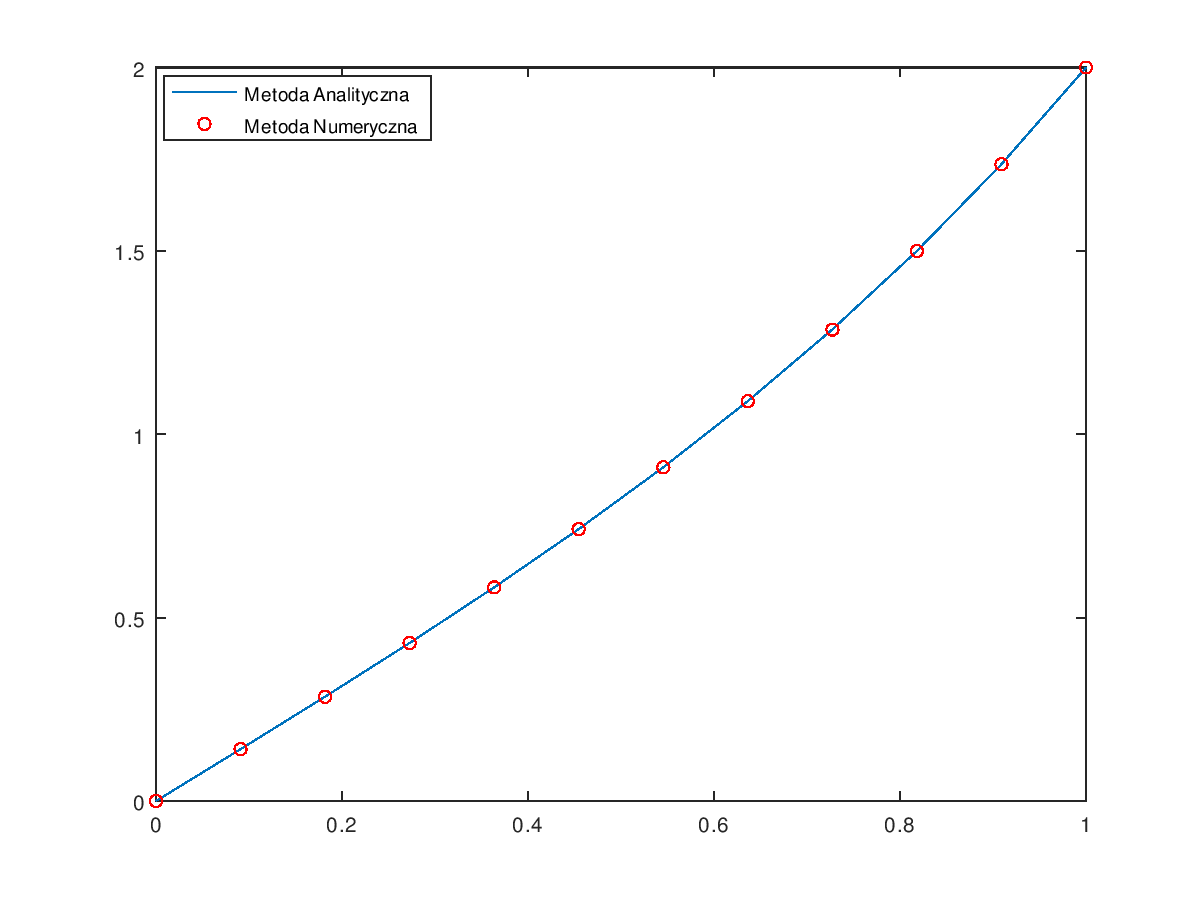
\includegraphics{Lab4/charts/zad1/zad1_n_10.png}
    
    %}
    \FloatBarrier
    \begin{figure}[!ht]
        \begin{center}
            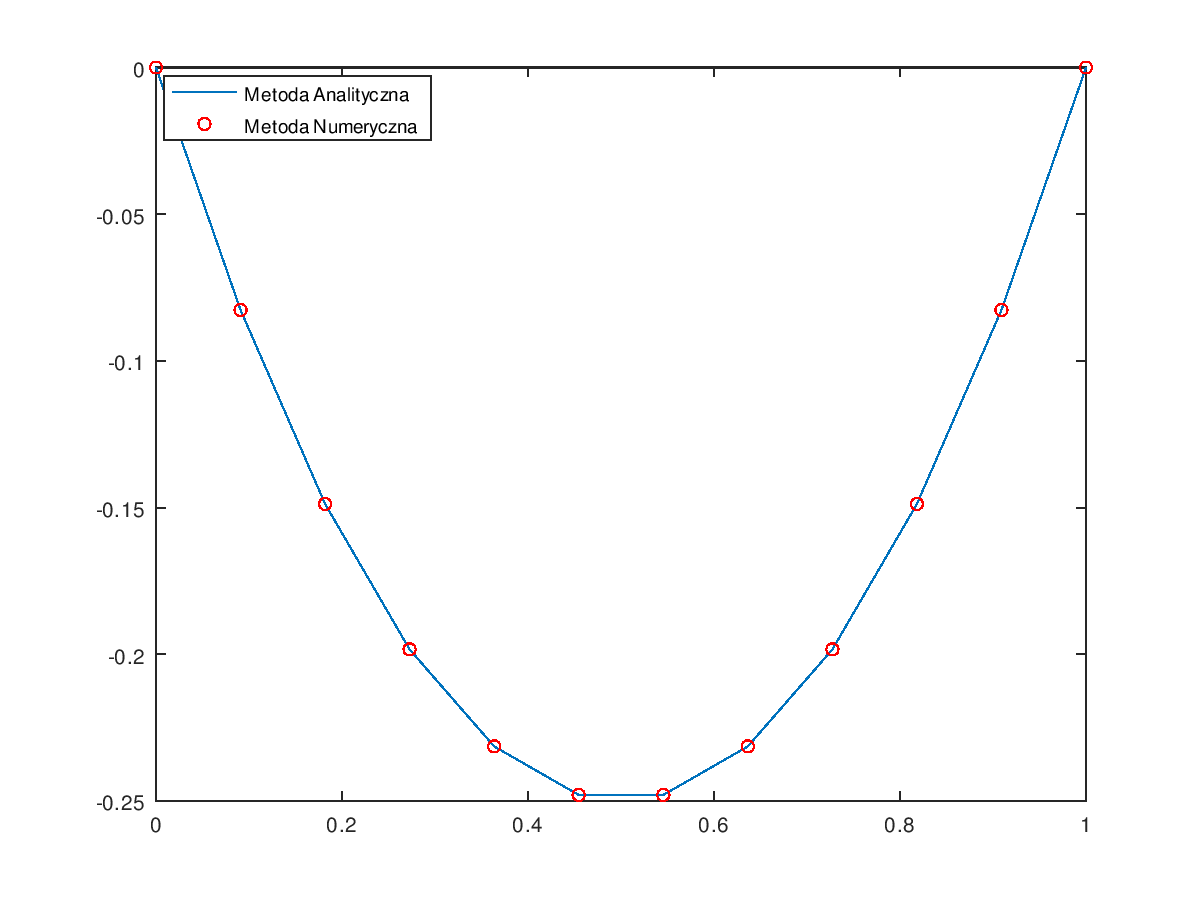
\includegraphics[width=0.8\textwidth]{Lab4/charts/zad3/zad3_n_10.png}
        \end{center}
        %\caption{Schemat logiczny w edytorze LAD oraz tabela symboli}
        %\label{fig:picture}
    \end{figure}
    \FloatBarrier
\end{samepage}

\begin{samepage}
    Dla 25 węzłów:
    \begin{figure}[!ht]
        \begin{center}
            \includegraphics[width=0.8\textwidth]{Lab4/charts/zad3/zad3_n_25.png}
        \end{center}
        %\caption{Schemat logiczny w edytorze LAD oraz tabela symboli}
        %\label{fig:picture}
    \end{figure}
    \FloatBarrier
\end{samepage}

\newpage
\begin{samepage}
    
    Dla 100 węzłów:
    \begin{figure}[!ht]
        \begin{center}
            \includegraphics[width=0.8\textwidth]{Lab4/charts/zad3/zad3_n_100.png}
        \end{center}
        %\caption{Schemat logiczny w edytorze LAD oraz tabela symboli}
        %\label{fig:picture}
    \end{figure}
    \FloatBarrier
\end{samepage}


\begin{samepage}
    Dla 1000 węzłów:
    
    \begin{figure}[!ht]
        \begin{center}
            \includegraphics[width=0.8\textwidth]{Lab4/charts/zad3/zad3_n_1000.png}
        \end{center}
        %\caption{Schemat logiczny w edytorze LAD oraz tabela symboli}
        %\label{fig:picture}
    \end{figure}
    \FloatBarrier
\end{samepage}    

\newpage

\begin{samepage}
    Błąd metody w zależności od liczby węzłów:
    \begin{figure}[!ht]
        \begin{center}
            \includegraphics[width=0.8\textwidth]{Lab4/charts/zad3/error_dane.png}
        \end{center}
        %\caption{Schemat logiczny w edytorze LAD oraz tabela symboli}
        %\label{fig:picture}
    \end{figure}
    \FloatBarrier
\end{samepage} 

\begin{samepage}
	\begin{figure}[!ht]
		\begin{center}
			\includegraphics[width=0.8\textwidth]{Lab4/charts/zad3/error.png}
		\end{center}
		%\caption{Schemat logiczny w edytorze LAD oraz tabela symboli}
		%\label{fig:picture}
	\end{figure}
	\FloatBarrier
\end{samepage} 

\subsection{Warunki brzegowe typu Neumanna}
\textbf{Postać ogólna zagadnień brzegowych rzędu II z warunkami brzegowymi typu Neumanna:}

\[
\begin{cases}
\vspace{0.1cm} 
\hspace{0,1cm} a(x) u'' + b(x)u' + c(x)u =f(x) \\
\vspace{0.1cm}
\hspace{0,1cm}u'|_{x=a} = \widetilde{u}_{a} \\
\hspace{0,1cm}u|_{x=b} = u_{b}
\end{cases}
\]
, gdzie:
$x\in[a,b]$

$a(x), b(x), c(x), f(x)$ są znanymi funkcjami

$u = u(x)$ jest poszukiwanym rozwiązaniem
\newline

\subsection{Cel ćwiczenia}
Kolejnym zadaniem było stworzenie algorytmów rozwiązujących zagadnienia brzegowe II rzędu z warunkami brzegowymi typu Neumanna.
\\\\
a) Pierwszego podejście polegało na wykorzystaniu schematu jednostronnego w celu aproksymacji pochodnej rzędu I występującej w warunku brzegowym typu Neumanna
\newpage
b) Drugie podejście polegało na dołączeniu dodatkowego węzła o indeksie (-1), który w rzeczywistości nie występuje w układzie równań
\\\\
c) Trzecie podejście polegało na wykorzystaniu jednostronnych schematów w węźle brzegowym
%\newpage

Do rozwiązania zostało podane następujące zagadnienie:
\[
\begin{cases}
\vspace{0.1cm} 
\hspace{0,1cm}u''-xu' + u=e^x(-x^2+x+2) \\
\vspace{0.1cm}
\hspace{0,1cm}u|_{x=0}=0 \\
\hspace{0,1cm}u'|_{x=1}=2e
\end{cases}
\]
, gdzie:

$x\in [0,1]$
\\
\\
Rozwiązanie analityczne: $\widetilde{u}(x) = (x+1)e^x$

\subsection{Rozwiązanie}


\begin{samepage}
a)
\input{Lab4/zad4_1}
\end{samepage}
\newpage
\begin{samepage}
b)
\input{Lab4/zad4_2}
\end{samepage}
\newpage
\begin{samepage}
c)
\input{Lab4/zad4_3}
\end{samepage}

\newpage

\subsection{Wykresy}

a)\\
\begin{samepage}
	Dla 10 węzłów:
	
	%{\centering
	
	%   \includegraphics{Lab4/charts/zad1/zad1_n_10.png}
	
	%}
	\FloatBarrier
	\begin{figure}[!ht]
		\begin{center}
			\includegraphics[width=0.8\textwidth]{Lab4/charts/zad4/1/10.png}
		\end{center}
		%\caption{Schemat logiczny w edytorze LAD oraz tabela symboli}
		%\label{fig:picture}
	\end{figure}
	\FloatBarrier
\end{samepage}

\begin{samepage}
	Dla 25 węzłów:
	\begin{figure}[!ht]
		\begin{center}
			\includegraphics[width=0.8\textwidth]{Lab4/charts/zad4/1/25.png}
		\end{center}
		%\caption{Schemat logiczny w edytorze LAD oraz tabela symboli}
		%\label{fig:picture}
	\end{figure}
	\FloatBarrier
\end{samepage}

\newpage
\begin{samepage}
	
	Dla 100 węzłów:
	\begin{figure}[!ht]
		\begin{center}
			\includegraphics[width=0.8\textwidth]{Lab4/charts/zad4/1/100.png}
		\end{center}
		%\caption{Schemat logiczny w edytorze LAD oraz tabela symboli}
		%\label{fig:picture}
	\end{figure}
	\FloatBarrier
\end{samepage}

\begin{samepage}
	Dla 1000 węzłów:
	
	\begin{figure}[!ht]
		\begin{center}
			\includegraphics[width=0.8\textwidth]{Lab4/charts/zad4/1/1000.png}
		\end{center}
		%\caption{Schemat logiczny w edytorze LAD oraz tabela symboli}
		%\label{fig:picture}
	\end{figure}
	\FloatBarrier
\end{samepage}    

\newpage

\begin{samepage}
	Błąd metody w zależności od liczby węzłów:
	\begin{figure}[!ht]
		\begin{center}
			\includegraphics[width=0.8\textwidth]{Lab4/charts/zad4/1/error_dane.png}
		\end{center}
		%\caption{Schemat logiczny w edytorze LAD oraz tabela symboli}
		%\label{fig:picture}
	\end{figure}
	\FloatBarrier
\end{samepage} 

\begin{samepage}
	
	\begin{figure}[!ht]
		\begin{center}
			\includegraphics[width=0.8\textwidth]{Lab4/charts/zad4/1/error.png}
		\end{center}
		%\caption{Schemat logiczny w edytorze LAD oraz tabela symboli}
		%\label{fig:picture}
	\end{figure}
	\FloatBarrier
\end{samepage} 

\newpage

b)\\
\begin{samepage}
	Dla 10 węzłów:
	
	%{\centering
	
	%   \includegraphics{Lab4/charts/zad1/zad1_n_10.png}
	
	%}
	\FloatBarrier
	\begin{figure}[!ht]
		\begin{center}
			\includegraphics[width=0.8\textwidth]{Lab4/charts/zad4/2/10.png}
		\end{center}
		%\caption{Schemat logiczny w edytorze LAD oraz tabela symboli}
		%\label{fig:picture}
	\end{figure}
	\FloatBarrier
\end{samepage}

\begin{samepage}
	Dla 25 węzłów:
	\begin{figure}[!ht]
		\begin{center}
			\includegraphics[width=0.8\textwidth]{Lab4/charts/zad4/2/25.png}
		\end{center}
		%\caption{Schemat logiczny w edytorze LAD oraz tabela symboli}
		%\label{fig:picture}
	\end{figure}
	\FloatBarrier
\end{samepage}

\newpage
\begin{samepage}
	
	Dla 100 węzłów:
	\begin{figure}[!ht]
		\begin{center}
			\includegraphics[width=0.8\textwidth]{Lab4/charts/zad4/2/100.png}
		\end{center}
		%\caption{Schemat logiczny w edytorze LAD oraz tabela symboli}
		%\label{fig:picture}
	\end{figure}
	\FloatBarrier
\end{samepage}

\begin{samepage}
	Dla 1000 węzłów:
	
	\begin{figure}[!ht]
		\begin{center}
			\includegraphics[width=0.8\textwidth]{Lab4/charts/zad4/2/1000.png}
		\end{center}
		%\caption{Schemat logiczny w edytorze LAD oraz tabela symboli}
		%\label{fig:picture}
	\end{figure}
	\FloatBarrier
\end{samepage}    

\newpage

\begin{samepage}
	Błąd metody w zależności od liczby węzłów:
	\begin{figure}[!ht]
		\begin{center}
			\includegraphics[width=0.8\textwidth]{Lab4/charts/zad4/2/error_dane.png}
		\end{center}
		%\caption{Schemat logiczny w edytorze LAD oraz tabela symboli}
		%\label{fig:picture}
	\end{figure}
	\FloatBarrier
\end{samepage} 

\begin{samepage}
	
	\begin{figure}[!ht]
		\begin{center}
			\includegraphics[width=0.8\textwidth]{Lab4/charts/zad4/2/error.png}
		\end{center}
		%\caption{Schemat logiczny w edytorze LAD oraz tabela symboli}
		%\label{fig:picture}
	\end{figure}
	\FloatBarrier
\end{samepage} 

\newpage

c)\\
\begin{samepage}
	Dla 10 węzłów:
	
	%{\centering
	
	%   \includegraphics{Lab4/charts/zad1/zad1_n_10.png}
	
	%}
	\FloatBarrier
	\begin{figure}[!ht]
		\begin{center}
			\includegraphics[width=0.8\textwidth]{Lab4/charts/zad4/3/10.png}
		\end{center}
		%\caption{Schemat logiczny w edytorze LAD oraz tabela symboli}
		%\label{fig:picture}
	\end{figure}
	\FloatBarrier
\end{samepage}

\begin{samepage}
	Dla 25 węzłów:
	\begin{figure}[!ht]
		\begin{center}
			\includegraphics[width=0.8\textwidth]{Lab4/charts/zad4/3/25.png}
		\end{center}
		%\caption{Schemat logiczny w edytorze LAD oraz tabela symboli}
		%\label{fig:picture}
	\end{figure}
	\FloatBarrier
\end{samepage}

\newpage
\begin{samepage}
	
	Dla 100 węzłów:
	\begin{figure}[!ht]
		\begin{center}
			\includegraphics[width=0.8\textwidth]{Lab4/charts/zad4/3/100.png}
		\end{center}
		%\caption{Schemat logiczny w edytorze LAD oraz tabela symboli}
		%\label{fig:picture}
	\end{figure}
	\FloatBarrier
\end{samepage}

\begin{samepage}
	Dla 1000 węzłów:
	
	\begin{figure}[!ht]
		\begin{center}
			\includegraphics[width=0.8\textwidth]{Lab4/charts/zad4/3/1000.png}
		\end{center}
		%\caption{Schemat logiczny w edytorze LAD oraz tabela symboli}
		%\label{fig:picture}
	\end{figure}
	\FloatBarrier
\end{samepage}    

\newpage

\begin{samepage}
	Błąd metody w zależności od liczby węzłów:
	\begin{figure}[!ht]
		\begin{center}
			\includegraphics[width=0.8\textwidth]{Lab4/charts/zad4/3/error_dane.png}
		\end{center}
		%\caption{Schemat logiczny w edytorze LAD oraz tabela symboli}
		%\label{fig:picture}
	\end{figure}
	\FloatBarrier
\end{samepage} 

\begin{samepage}
	
	\begin{figure}[!ht]
		\begin{center}
			\includegraphics[width=0.8\textwidth]{Lab4/charts/zad4/3/error.png}
		\end{center}
		%\caption{Schemat logiczny w edytorze LAD oraz tabela symboli}
		%\label{fig:picture}
	\end{figure}
	\FloatBarrier
\end{samepage} 

\newpage




    
    %\section{Równania różniczkowe cząstkowe I i II rzędu}
\subsection{Równania różniczkowe liniowe rzędu II}
Równanie różniczkowe postaci:
$$ a(x,y) \dfrac{\partial^2u}{\partial x^2} + 2b \dfrac{\partial ^2u}{\partial x \partial u} + c(x,y)\dfrac{\partial^2u}{\partial y^2} + d(x,y) \dfrac{\partial u}{\partial x} + e(x,y) \dfrac{\partial u}{\partial y} + f(x,y) u + g(x,y) = 0$$

nazywamy równaniem różniczkowym cząstkowym liniowym rzędu II, gdzie $a^2 + b^2 + c^2>0$ na $\Omega$,\\ a, b, c, d, e, f, g $\in$ C($\Omega$)
\\
\\
Wyróżnik równania cząstkowego rzędu II:
$$\Delta = b^2 = ac$$\\
Równanie różniczkowe cząstkowe liniowe rzędu II jest typu eliptycznego, gdy $\Delta < 0$

\subsection{Cel ćwiczenia}
Naszym zadaniem było rozwiązanie równań Laplace'a i Poissona z dwuwymiarowymi zagadnieniami Dirichletta za pomocą stworzonego przez nas programu.
\\
\\
Równanie Poissona z dwuwymiarowymi zagadnieniami Dirichletta jest równaniem eliptycznym postaci:
\[
\begin{cases}
\vspace{0.1cm} 
\hspace{0,1cm}\dfrac{\partial^2 u}{\partial x^2} + \dfrac{\partial^2 u}{\partial y^2} = f\\
\vspace{0.1cm}
\hspace{0,1cm}u_{|\partial \Omega} = \widetilde{u} \\
\end{cases}
\]

, gdzie:

$(x,y) \in \Omega$

$\Omega = [a,b] \times [c,d]$

$\Omega \subset \Re^2$

Postać równania Laplace'a otrzymujemy przez podstawienie do równania Poissona $f \equiv 0$. \\

Wykorzystując schemat 5-pkt. dla operatora Laplace'a otrzymujemy odpowiednie równania:\\

\begin{enumerate}
	\item Dla siatki równomiernej (h=k)
	\begin{equation}
-4u_{i,j} + u_{i+1,j} + u_{i-1,j} + u_{i,j+1} + u_{i,j-1} = h^2 f_{i,j} \tag{*}
	\end{equation}
	
	\item Dla siatki nierównomiernej (h $\neq$ k)
	\begin{equation}
		\dfrac{1}{h^2}\left(u_{i+1,j} + u_{i-1,j} \right) + \dfrac{1}{k^2} \left(u_{i,j+1} + u_{i,j-1} \right) -2\left(\dfrac{1}{h^2} + \dfrac{1}{k^2} \right)u_{i,j} = f_{i,j} \tag{**}
	\end{equation}	
\end{enumerate}
Stosując równanie (**) otrzymujemy ogólniejsze rozwiązanie, ponieważ równienie (*) otrzymujemy przez podstawnie $k=h$ oraz odpowiednie przekształcenia.
\\	

Rozwiązaliśmy następujące równania:
\begin{multicols}{3}
	a)\\\\$\dfrac{\partial^2 u}{\partial x^2} + \dfrac{\partial^2 u}{\partial y^2} = 0$\vspace{0.2cm}\\\\, gdzie:\\
	$\Omega = [0,1]\times[0,1]$\\
	warunki brzegowe:\\
	$u(x,0) = 0$\\
	$u(1,y) = y$\\
	$u(x,1) = x$\\
	$u(0,y) = 0$
	\vspace{0.1cm}\\
	Rozwiązanie analityczne:\\
	\columnbreak
	$\widetilde{u}(x,y) = xy$\\
	b)\\\\$\dfrac{\partial^2 u}{\partial x^2} + \dfrac{\partial^2 u}{\partial y^2} = (x^2+y^2)e^{xy}$\vspace{0.2cm}\\\\, gdzie:\\
	$\Omega = [0,2]\times[0,1]$\\
	warunki brzegowe:\\
	$u(x,0) = 1$\\
	$u(2,y) = e^{2y}$\\
	$u(x,1) = e^x$\\	
	$u(0,y) = 1$
	\vspace{0.1cm}\\
	Rozwiązanie analityczne:\\
	\columnbreak
	$\widetilde{u}(x,y) = e^{xy}$\\
	c)\\\\$\dfrac{\partial^2 u}{\partial x^2} + \dfrac{\partial^2 u}{\partial y^2} = \dfrac{x}{y} + \dfrac{y}{x}$\vspace{0cm}\\\\, gdzie:\\
	$\Omega = [1,2]\times[1,2]$\\
	warunki brzegowe:\\
	$u(x,1) = x\cdot lnx$\\
	$u(2,y) = 2y\cdot ln(2y)$\\
	$u(x,2) = x\cdot ln(4x^2)$\\
	$u(1,y) = y\cdot lny$
	\vspace{0.1cm}\\
	Rozwiązanie analityczne:\\
	$\widetilde{u}(x,y) = xy\cdot ln(xy)$
	
	
\end{multicols}

\subsection{Algorytm}

\begin{samepage}
%\begin{Shaded}
\begin{Highlighting}[]
\FunctionTok{clear}\NormalTok{, }\FunctionTok{clc}\NormalTok{;}
\CommentTok{% zad 3}
\CommentTok{% Przykładowe dane}
\NormalTok{nx = }\FloatTok{10}\NormalTok{; ny = }\FloatTok{10}\NormalTok{; xa = }\FloatTok{0}\NormalTok{; xb = }\FloatTok{2}\NormalTok{; ya = }\FloatTok{0}\NormalTok{; yb = }\FloatTok{1}\NormalTok{;}
\NormalTok{f = @(x, y) (x.^}\FloatTok{2} \NormalTok{+ y.^}\FloatTok{2}\NormalTok{) .* }\FunctionTok{exp}\NormalTok{(x.*y);}
\NormalTok{g = @(x, y) }\FunctionTok{exp}\NormalTok{(x.*y);}
\NormalTok{uxa = @(x) }\FloatTok{1}\NormalTok{;         }\CommentTok{%u1}
\NormalTok{uxb = @(x) }\FunctionTok{exp}\NormalTok{(x);    }\CommentTok{%u3}
\NormalTok{uya = @(y) }\FloatTok{1}\NormalTok{;         }\CommentTok{%u4}
\NormalTok{uyb = @(y) }\FunctionTok{exp}\NormalTok{(}\FloatTok{2}\NormalTok{.*y); }\CommentTok{%u2}

\CommentTok{% Obliczenia}
\NormalTok{h = (xb-xa)/(nx+}\FloatTok{1}\NormalTok{);}
\NormalTok{k = (yb-ya)/(ny+}\FloatTok{1}\NormalTok{);}
\NormalTok{xM = }\FunctionTok{linspace}\NormalTok{(xa + h, xb - h, nx);}
\NormalTok{yM  = }\FunctionTok{linspace}\NormalTok{(ya+k, yb-k, ny);}
\NormalTok{T = -}\FloatTok{4}\NormalTok{* }\FunctionTok{eye}\NormalTok{(nx) + }\FunctionTok{diag}\NormalTok{(}\FunctionTok{diag}\NormalTok{(}\FunctionTok{eye}\NormalTok{(nx-}\FloatTok{1}\NormalTok{)),-}\FloatTok{1}\NormalTok{) + }\FunctionTok{diag}\NormalTok{(}\FunctionTok{diag}\NormalTok{(}\FunctionTok{eye}\NormalTok{(nx-}\FloatTok{1}\NormalTok{)),}\FloatTok{1}\NormalTok{);}
\BaseNTok{I} \NormalTok{= }\FunctionTok{eye}\NormalTok{(nx);}
\NormalTok{B = }\FunctionTok{kron}\NormalTok{(}\FunctionTok{eye}\NormalTok{(ny), T);}
\NormalTok{C = }\FunctionTok{kron}\NormalTok{(}\FunctionTok{diag}\NormalTok{(}\FunctionTok{diag}\NormalTok{(}\FunctionTok{eye}\NormalTok{(ny-}\FloatTok{1}\NormalTok{)),-}\FloatTok{1}\NormalTok{), }\BaseNTok{I}\NormalTok{);}
\NormalTok{D = }\FunctionTok{kron}\NormalTok{(}\FunctionTok{diag}\NormalTok{(}\FunctionTok{diag}\NormalTok{(}\FunctionTok{eye}\NormalTok{(ny-}\FloatTok{1}\NormalTok{)),}\FloatTok{1}\NormalTok{), }\BaseNTok{I}\NormalTok{);}
\NormalTok{A = B + C + D;}

\NormalTok{[X1 Y1] = }\FunctionTok{meshgrid}\NormalTok{(xM,yM);}
\NormalTok{F = f(X1, Y1)' .* }\FunctionTok{ones}\NormalTok{(nx, ny);}
\NormalTok{F = h^}\FloatTok{2} \NormalTok{.* F;}
\NormalTok{F(:, }\FloatTok{1}\NormalTok{) = F(:, }\FloatTok{1}\NormalTok{) - uxa(xM)';}
\NormalTok{F(:, ny) = F(:, ny) - uxb(xM)';}
\NormalTok{F(}\FloatTok{1}\NormalTok{, :) = F(}\FloatTok{1}\NormalTok{, :) - uya(yM);}
\NormalTok{F(nx, :) = F(nx, :) - uyb(yM);}
\NormalTok{F = }\FunctionTok{reshape}\NormalTok{(F,  nx*ny, }\FloatTok{1}\NormalTok{);}
\CommentTok{% Rozwiązanie}
\NormalTok{U = linsolve(A,F);}
\NormalTok{U = }\FunctionTok{reshape}\NormalTok{(U,  nx, ny)';}
\NormalTok{[X,Y] = }\FunctionTok{meshgrid}\NormalTok{(xa:h:xb, ya:k:yb);}
\NormalTok{U = [uya(yM)' .* }\FunctionTok{diag}\NormalTok{(}\FunctionTok{eye}\NormalTok{(ny)), U, uyb(yM)' .* }\FunctionTok{diag}\NormalTok{(}\FunctionTok{eye}\NormalTok{(ny))];}
\NormalTok{XM = [xa xM xb];}
\NormalTok{G = g(X,Y);}
\NormalTok{U = [uxa(XM)' .* }\FunctionTok{diag}\NormalTok{(}\FunctionTok{eye}\NormalTok{(nx+}\FloatTok{2}\NormalTok{)), U', uxb(XM)' .* }\FunctionTok{diag}\NormalTok{(}\FunctionTok{eye}\NormalTok{(nx+}\FloatTok{2}\NormalTok{))]';}
\CommentTok{% Błąd}
\NormalTok{Error = }\FunctionTok{max}\NormalTok{(}\FunctionTok{max}\NormalTok{(}\FunctionTok{abs}\NormalTok{(G-U)));}
\CommentTok{% Wykres}
\FunctionTok{subplot}\NormalTok{(}\FloatTok{1}\NormalTok{,}\FloatTok{2}\NormalTok{,}\FloatTok{1}\NormalTok{)}
\FunctionTok{surf}\NormalTok{(X,Y,U)}
\FunctionTok{subplot}\NormalTok{(}\FloatTok{1}\NormalTok{,}\FloatTok{2}\NormalTok{,}\FloatTok{2}\NormalTok{)}
\FunctionTok{surf}\NormalTok{(X,Y,G)}
\end{Highlighting}
\end{Shaded}
 złe zmienić na nowe!
\begin{Shaded}
\begin{Highlighting}[]
\FunctionTok{clear}\NormalTok{, }\FunctionTok{clc}\NormalTok{;}
\CommentTok{% zad 2}
\CommentTok{% Przykładowe dane}
\NormalTok{nx = }\FloatTok{10}\NormalTok{; ny = }\FloatTok{50}\NormalTok{; xa = }\FloatTok{0}\NormalTok{; xb = }\FloatTok{2}\NormalTok{; ya = }\FloatTok{0}\NormalTok{; yb = }\FloatTok{1}\NormalTok{;}
\NormalTok{f = @(x, y) (x.^}\FloatTok{2}\NormalTok{ + y.^}\FloatTok{2}\NormalTok{) .* }\FunctionTok{exp}\NormalTok{(x.*y);}
\NormalTok{g = @(x, y) }\FunctionTok{exp}\NormalTok{(x.*y);}
\NormalTok{uxa = @(x) }\FloatTok{1}\NormalTok{;         }\CommentTok{%u1}
\NormalTok{uxb = @(x) }\FunctionTok{exp}\NormalTok{(x);    }\CommentTok{%u3}
\NormalTok{uya = @(y) }\FloatTok{1}\NormalTok{;         }\CommentTok{%u4}
\NormalTok{uyb = @(y) }\FunctionTok{exp}\NormalTok{(}\FloatTok{2}\NormalTok{.*y); }\CommentTok{%u2}

\CommentTok{% Obliczenia}
\NormalTok{h = (xb-xa)/(nx+}\FloatTok{1}\NormalTok{);}
\NormalTok{k = (yb-ya)/(ny+}\FloatTok{1}\NormalTok{);}
\NormalTok{xM = }\FunctionTok{linspace}\NormalTok{(xa + h, xb - h, nx);}
\NormalTok{yM  = }\FunctionTok{linspace}\NormalTok{(ya+k, yb-k, ny);}
\NormalTok{T = -}\FloatTok{2}\NormalTok{*(h^}\FloatTok{2}\NormalTok{ + k^}\FloatTok{2}\NormalTok{) * }\FunctionTok{eye}\NormalTok{(nx) + k^}\FloatTok{2}\NormalTok{ * }\FunctionTok{diag}\NormalTok{(}\FunctionTok{diag}\NormalTok{(}\FunctionTok{eye}\NormalTok{(nx-}\FloatTok{1}\NormalTok{)),-}\FloatTok{1}\NormalTok{) \textbackslash{}}
\NormalTok{+ k^}\FloatTok{2}\NormalTok{ * }\FunctionTok{diag}\NormalTok{(}\FunctionTok{diag}\NormalTok{(}\FunctionTok{eye}\NormalTok{(nx-}\FloatTok{1}\NormalTok{)),}\FloatTok{1}\NormalTok{);}
\BaseNTok{I}\NormalTok{ = }\FunctionTok{eye}\NormalTok{(nx);}
\NormalTok{B = }\FunctionTok{kron}\NormalTok{(}\FunctionTok{eye}\NormalTok{(ny), T);}
\NormalTok{C = }\FunctionTok{kron}\NormalTok{(}\FunctionTok{diag}\NormalTok{(}\FunctionTok{diag}\NormalTok{(}\FunctionTok{eye}\NormalTok{(ny-}\FloatTok{1}\NormalTok{)),-}\FloatTok{1}\NormalTok{), h^}\FloatTok{2}\NormalTok{ * }\BaseNTok{I}\NormalTok{);}
\NormalTok{D = }\FunctionTok{kron}\NormalTok{(}\FunctionTok{diag}\NormalTok{(}\FunctionTok{diag}\NormalTok{(}\FunctionTok{eye}\NormalTok{(ny-}\FloatTok{1}\NormalTok{)),}\FloatTok{1}\NormalTok{), h^}\FloatTok{2}\NormalTok{ * }\BaseNTok{I}\NormalTok{);}
\NormalTok{A = B + C + D;}

\NormalTok{[X1 Y1] = }\FunctionTok{meshgrid}\NormalTok{(xM,yM);}
\NormalTok{F = f(X1, Y1)' .* }\FunctionTok{ones}\NormalTok{(nx, ny);}
\NormalTok{F = h^}\FloatTok{2}\NormalTok{ * k^}\FloatTok{2}\NormalTok{ .* F;}
\NormalTok{F(:, }\FloatTok{1}\NormalTok{) = F(:, }\FloatTok{1}\NormalTok{) - h^}\FloatTok{2}\NormalTok{ * uxa(xM)';}
\NormalTok{F(:, ny) = F(:, ny) - h^}\FloatTok{2}\NormalTok{ * uxb(xM)';}
\NormalTok{F(}\FloatTok{1}\NormalTok{, :) = F(}\FloatTok{1}\NormalTok{, :) - k^}\FloatTok{2}\NormalTok{ * uya(yM);}
\NormalTok{F(nx, :) = F(nx, :) - k^}\FloatTok{2}\NormalTok{ * uyb(yM);}
\NormalTok{F = }\FunctionTok{reshape}\NormalTok{(F,  nx*ny, }\FloatTok{1}\NormalTok{);}
\CommentTok{% Rozwiązanie}
\NormalTok{U = linsolve(A,F);}
\NormalTok{U = }\FunctionTok{reshape}\NormalTok{(U,  nx, ny)';}
\NormalTok{[X,Y] = }\FunctionTok{meshgrid}\NormalTok{(xa:h:xb, ya:k:yb);}
\NormalTok{U = [uya(yM)' .* }\FunctionTok{diag}\NormalTok{(}\FunctionTok{eye}\NormalTok{(ny)), U, uyb(yM)' .* }\FunctionTok{diag}\NormalTok{(}\FunctionTok{eye}\NormalTok{(ny))];}
\NormalTok{XM = [xa xM xb];}
\NormalTok{G = g(X,Y);}
\NormalTok{U = [uxa(XM)' .* }\FunctionTok{diag}\NormalTok{(}\FunctionTok{eye}\NormalTok{(nx+}\FloatTok{2}\NormalTok{)), U', uxb(XM)' .* }\FunctionTok{diag}\NormalTok{(}\FunctionTok{eye}\NormalTok{(nx+}\FloatTok{2}\NormalTok{))]';}
\CommentTok{% Błąd}
\NormalTok{Error = }\FunctionTok{max}\NormalTok{(}\FunctionTok{max}\NormalTok{(}\FunctionTok{abs}\NormalTok{(G-U)));}
\CommentTok{% Wykres}
\FunctionTok{subplot}\NormalTok{(}\FloatTok{1}\NormalTok{,}\FloatTok{2}\NormalTok{,}\FloatTok{1}\NormalTok{)}
\FunctionTok{surf}\NormalTok{(X,Y,U)}
\FunctionTok{subplot}\NormalTok{(}\FloatTok{1}\NormalTok{,}\FloatTok{2}\NormalTok{,}\FloatTok{2}\NormalTok{)}
\FunctionTok{surf}\NormalTok{(X,Y,G)}
\end{Highlighting}
\end{Shaded}
\end{samepage}

\newpage

\subsection{Wykresy}

a)

Dla nx = ny = 5:

\begin{figure}[!ht]
	\begin{center}
		\includegraphics[width=0.78\textwidth]{Lab5/charts/zad1/5x5.png}
	\end{center}
\end{figure}

Czas wykonywania algorytmu $ = 0.0136 s$

Dla nx = ny = 15:

\begin{figure}[!ht]
	\begin{center}
		\includegraphics[width=0.78\textwidth]{Lab5/charts/zad1/15x15.png}
	\end{center}
\end{figure}

Czas wykonywania algorytmu $ = 0.0155 s$

\newpage
Dla nx = ny = 30:

\begin{figure}[!ht]
	\begin{center}
		\includegraphics[width=0.8\textwidth]{Lab5/charts/zad1/30x30.png}
	\end{center}
\end{figure}

Czas wykonywania algorytmu $ = 0.0329 s$

Dla nx = ny = 100:

\begin{figure}[!ht]
	\begin{center}
		\includegraphics[width=0.8\textwidth]{Lab5/charts/zad1/100x100.png}
	\end{center}
\end{figure}

Czas wykonywania algorytmu $ = 6,370 s$

\newpage

Błąd metody w zależności od liczby węzłów:

\begin{figure}[!ht]
	\begin{center}
		\includegraphics[width=0.8\textwidth]{Lab5/charts/zad1/error_dane.png}
	\end{center}
\end{figure}

\begin{figure}[!ht]
	\begin{center}
		\includegraphics[width=0.8\textwidth]{Lab5/charts/zad1/error.png}
	\end{center}
\end{figure}

\newpage

Dla siatek nierównomiernych:

Dla nx = 5, ny = 50:

\begin{figure}[!ht]
	\begin{center}
		\includegraphics[width=0.8\textwidth]{Lab5/charts/zad1/5x50.png}
	\end{center}
\end{figure}

Czas wykonywania algorytmu $ = 0.014 s$

Błąd $3.8858e-15$

Dla nx = 50, ny = 5:

\begin{figure}[!ht]
	\begin{center}
		\includegraphics[width=0.8\textwidth]{Lab5/charts/zad1/50x5.png}
	\end{center}
\end{figure}

Czas wykonywania algorytmu $ = 0.014 s$

Błąd $4.2188e-15$

\newpage

b)

Dla nx = ny = 5:

\begin{figure}[!ht]
	\begin{center}
		\includegraphics[width=0.78\textwidth]{Lab5/charts/zad2/5x5.png}
	\end{center}
\end{figure}

Czas wykonywania algorytmu $ = 0.0140 s$

Dla nx = ny = 15:

\begin{figure}[!ht]
	\begin{center}
		\includegraphics[width=0.78\textwidth]{Lab5/charts/zad2/15x15.png}
	\end{center}
\end{figure}

Czas wykonywania algorytmu $ = 0.0157 s$

\newpage
Dla nx = ny = 30:

\begin{figure}[!ht]
	\begin{center}
		\includegraphics[width=0.8\textwidth]{Lab5/charts/zad2/30x30.png}
	\end{center}
\end{figure}

Czas wykonywania algorytmu $ = 0.0320 s$

Dla nx = ny = 100:

\begin{figure}[!ht]
	\begin{center}
		\includegraphics[width=0.8\textwidth]{Lab5/charts/zad2/100x100.png}
	\end{center}
\end{figure}

Czas wykonywania algorytmu $ = 6,605 s$

\newpage

Błąd metody w zależności od liczby węzłów:

\begin{figure}[!ht]
	\begin{center}
		\includegraphics[width=0.8\textwidth]{Lab5/charts/zad2/error_dane.png}
	\end{center}
\end{figure}

\begin{figure}[!ht]
	\begin{center}
		\includegraphics[width=0.8\textwidth]{Lab5/charts/zad2/error.png}
	\end{center}
\end{figure}

\newpage

Dla siatek nierównomiernych:

Dla nx = 5, ny = 50:

\begin{figure}[!ht]
	\begin{center}
		\includegraphics[width=0.8\textwidth]{Lab5/charts/zad2/5x50.png}
	\end{center}
\end{figure}

Czas wykonywania algorytmu $ = 0.164 s$

Błąd $4.5862e-04$

Dla nx = 50, ny = 5:

\begin{figure}[!ht]
	\begin{center}
		\includegraphics[width=0.8\textwidth]{Lab5/charts/zad2/50x5.png}
	\end{center}
\end{figure}

Czas wykonywania algorytmu $ = 0.0167 s$

Błąd $0.0028$

\newpage

c)

Dla nx = ny = 5:

\begin{figure}[!ht]
	\begin{center}
		\includegraphics[width=0.78\textwidth]{Lab5/charts/zad3/5x5.png}
	\end{center}
\end{figure}

Czas wykonywania algorytmu $ = 0.0148 s$

Dla nx = ny = 15:

\begin{figure}[!ht]
	\begin{center}
		\includegraphics[width=0.78\textwidth]{Lab5/charts/zad3/15x15.png}
	\end{center}
\end{figure}

Czas wykonywania algorytmu $ = 0.0159 s$

\newpage
Dla nx = ny = 30:

\begin{figure}[!ht]
	\begin{center}
		\includegraphics[width=0.8\textwidth]{Lab5/charts/zad3/30x30.png}
	\end{center}
\end{figure}

Czas wykonywania algorytmu $ = 0.0363 s$

Dla nx = ny = 100:

\begin{figure}[!ht]
	\begin{center}
		\includegraphics[width=0.8\textwidth]{Lab5/charts/zad3/100x100.png}
	\end{center}
\end{figure}

Czas wykonywania algorytmu $ = 6,538 s$

\newpage

Błąd metody w zależności od liczby węzłów:

\begin{figure}[!ht]
	\begin{center}
		\includegraphics[width=0.8\textwidth]{Lab5/charts/zad3/error_dane.png}
	\end{center}
\end{figure}

\begin{figure}[!ht]
	\begin{center}
		\includegraphics[width=0.8\textwidth]{Lab5/charts/zad3/error.png}
	\end{center}
\end{figure}

\newpage

Dla siatek nierównomiernych:

Dla nx = 5, ny = 50:

\begin{figure}[!ht]
	\begin{center}
		\includegraphics[width=0.8\textwidth]{Lab5/charts/zad3/5x50.png}
	\end{center}
\end{figure}

Czas wykonywania algorytmu $ = 0.0159 s$

Błąd $1.8168e-04$

Dla nx = 50, ny = 5:

\begin{figure}[!ht]
	\begin{center}
		\includegraphics[width=0.8\textwidth]{Lab5/charts/zad3/50x5.png}
	\end{center}
\end{figure}

Czas wykonywania algorytmu $ = 0.0157 s$

Błąd $1.8168e-04$


\newpage
    
    \section{Iteracyjne metody rozwiązywania równań eliptycznych}

Będziemy korzystać z równania:

$$u_{i,j} = \frac{1}{4}(u_{i+1,j} + u_{i-1,j} + u_{i,j+1} + u_{i,j-1}) - \frac{1}{4}h^2f_{i,j}$$

\vspace{0.5cm}

Rozpatrzmy równanie:

\[
\begin{cases}
\vspace{0.1cm} 
\hspace{0,1cm}\dfrac{\partial^2 u}{\partial x^2} + \dfrac{\partial^2 u}{\partial y^2} = f\\
\vspace{0.1cm}
\hspace{0,1cm}u_{|\partial \Omega} = \widetilde{u} \\
\end{cases}
\]

, gdzie:

$(x,y) \in \Omega$

$\Omega = [a,b] \times [c,d]$

$\Omega \subset \Re^2$

\subsection{Cel ćwiczenia}

Naszym zadaniem było stworzenie algorytmu rozwiązującego następujące równania:

a) \hspace{6cm} b)

$\dfrac{\partial^2 u}{\partial x^2} + \dfrac{\partial^2 u}{\partial y^2} = 0$ \hspace{4.15cm} $\dfrac{\partial^2 u}{\partial x^2} + \dfrac{\partial^2 u}{\partial y^2} = -cos(x+y)-cos(x-y)$

, gdzie: \hspace{5.2cm} , gdzie:

warunki brzegowe: \hspace{3.5cm} warunki brzegowe:

$u(x,0) = 2lnx$ \hspace{4.15cm} $u(x,0) = cos(x)$

$u(1,y) = ln(y^2 + 1)$ \hspace{3.3cm} $u(0,y) = cos(y)$

$u(x,1) = ln(x^2 + 1)$ \hspace{3.28cm} $u(x,\frac{\pi}{2}) = 0$

$u(2,y) = ln(y^2 + 4)$ \hspace{3.3cm} $u(\pi,y) = -cos(y)$

rozwiązanie analityczne: \hspace{2.6cm} rozwiązanie analityczne:

$u(x,y) = ln(x^2 + y^2)$ \hspace{3.1cm} $u(x,y) = cos(x)\cdot cos(y)$

\vspace{0.5cm}

Trzema metodami: Jacobiego, Gaussa $-$ Seidela oraz nadrelaksacji Younge'a. Dodatkowo przedstawimy dwupoziomową metodę Peacemanna $-$ Rachforda.

\subsection{Metoda Jacobiego}

W metodzie tej wybieramy pierwsze arbitralne, dowolne przybliżenie rozwiązania numerycznego.

Im bliżej rozwiązania analitycznego dobrane jest przybliżenie tym mniej iteracji będziemy potrzebować w procesie iteracyjnym.

Jedna pełna iteracja polega na poprawieniu jeden raz wartości przybliżonych we wszystkich węzłach wewnętrznych siatki, aby następnie przejść do kolejnej iteracji wychodząc z tego samego węzła co poprzednio.

Dobór punktów nie ma znaczenia, ważne jest jedynie aby w kolejnych iteracjach zachować obrany porządek.

Zaletą metody Jacobiego jest nie generowanie wielkich macierzy; wadą dość wolna zbieżność.

Dowolne pierwsze przybliżenie:

$$u_{i,j}^{(n)} = \frac{1}{4}(u_{i+1,j}^{(n)} + u_{i-1,j}^{(n)} + u_{i,j+1}^{(n)} + u_{i,j-1}^{(n)}) - \frac{1}{4}h^2f_{i,j}$$

\subsubsection{Algorytm}

a)

\documentclass[]{article}
\usepackage{lmodern}
\usepackage{amssymb,amsmath}
\usepackage{ifxetex,ifluatex}
\usepackage{fixltx2e} % provides \textsubscript
\ifnum 0\ifxetex 1\fi\ifluatex 1\fi=0 % if pdftex
  \usepackage[T1]{fontenc}
  \usepackage[utf8]{inputenc}
\else % if luatex or xelatex
  \ifxetex
    \usepackage{mathspec}
  \else
    \usepackage{fontspec}
  \fi
  \defaultfontfeatures{Ligatures=TeX,Scale=MatchLowercase}
\fi
% use upquote if available, for straight quotes in verbatim environments
\IfFileExists{upquote.sty}{\usepackage{upquote}}{}
% use microtype if available
\IfFileExists{microtype.sty}{%
\usepackage{microtype}
\UseMicrotypeSet[protrusion]{basicmath} % disable protrusion for tt fonts
}{}
\usepackage[margin=1in]{geometry}
\usepackage{hyperref}
\hypersetup{unicode=true,
            pdftitle={Lab5},
            pdfauthor={Me},
            pdfborder={0 0 0},
            breaklinks=true}
\urlstyle{same}  % don't use monospace font for urls
\usepackage{color}
\usepackage{fancyvrb}
\newcommand{\VerbBar}{|}
\newcommand{\VERB}{\Verb[commandchars=\\\{\}]}
\DefineVerbatimEnvironment{Highlighting}{Verbatim}{commandchars=\\\{\}}
% Add ',fontsize=\small' for more characters per line
\usepackage{framed}
\definecolor{shadecolor}{RGB}{248,248,248}
\newenvironment{Shaded}{\begin{snugshade}}{\end{snugshade}}
\newcommand{\KeywordTok}[1]{\textcolor[rgb]{0.13,0.29,0.53}{\textbf{{#1}}}}
\newcommand{\DataTypeTok}[1]{\textcolor[rgb]{0.13,0.29,0.53}{{#1}}}
\newcommand{\DecValTok}[1]{\textcolor[rgb]{0.00,0.00,0.81}{{#1}}}
\newcommand{\BaseNTok}[1]{\textcolor[rgb]{0.00,0.00,0.81}{{#1}}}
\newcommand{\FloatTok}[1]{\textcolor[rgb]{0.00,0.00,0.81}{{#1}}}
\newcommand{\ConstantTok}[1]{\textcolor[rgb]{0.00,0.00,0.00}{{#1}}}
\newcommand{\CharTok}[1]{\textcolor[rgb]{0.31,0.60,0.02}{{#1}}}
\newcommand{\SpecialCharTok}[1]{\textcolor[rgb]{0.00,0.00,0.00}{{#1}}}
\newcommand{\StringTok}[1]{\textcolor[rgb]{0.31,0.60,0.02}{{#1}}}
\newcommand{\VerbatimStringTok}[1]{\textcolor[rgb]{0.31,0.60,0.02}{{#1}}}
\newcommand{\SpecialStringTok}[1]{\textcolor[rgb]{0.31,0.60,0.02}{{#1}}}
\newcommand{\ImportTok}[1]{{#1}}
\newcommand{\CommentTok}[1]{\textcolor[rgb]{0.56,0.35,0.01}{\textit{{#1}}}}
\newcommand{\DocumentationTok}[1]{\textcolor[rgb]{0.56,0.35,0.01}{\textbf{\textit{{#1}}}}}
\newcommand{\AnnotationTok}[1]{\textcolor[rgb]{0.56,0.35,0.01}{\textbf{\textit{{#1}}}}}
\newcommand{\CommentVarTok}[1]{\textcolor[rgb]{0.56,0.35,0.01}{\textbf{\textit{{#1}}}}}
\newcommand{\OtherTok}[1]{\textcolor[rgb]{0.56,0.35,0.01}{{#1}}}
\newcommand{\FunctionTok}[1]{\textcolor[rgb]{0.00,0.00,0.00}{{#1}}}
\newcommand{\VariableTok}[1]{\textcolor[rgb]{0.00,0.00,0.00}{{#1}}}
\newcommand{\ControlFlowTok}[1]{\textcolor[rgb]{0.13,0.29,0.53}{\textbf{{#1}}}}
\newcommand{\OperatorTok}[1]{\textcolor[rgb]{0.81,0.36,0.00}{\textbf{{#1}}}}
\newcommand{\BuiltInTok}[1]{{#1}}
\newcommand{\ExtensionTok}[1]{{#1}}
\newcommand{\PreprocessorTok}[1]{\textcolor[rgb]{0.56,0.35,0.01}{\textit{{#1}}}}
\newcommand{\AttributeTok}[1]{\textcolor[rgb]{0.77,0.63,0.00}{{#1}}}
\newcommand{\RegionMarkerTok}[1]{{#1}}
\newcommand{\InformationTok}[1]{\textcolor[rgb]{0.56,0.35,0.01}{\textbf{\textit{{#1}}}}}
\newcommand{\WarningTok}[1]{\textcolor[rgb]{0.56,0.35,0.01}{\textbf{\textit{{#1}}}}}
\newcommand{\AlertTok}[1]{\textcolor[rgb]{0.94,0.16,0.16}{{#1}}}
\newcommand{\ErrorTok}[1]{\textcolor[rgb]{0.64,0.00,0.00}{\textbf{{#1}}}}
\newcommand{\NormalTok}[1]{{#1}}
\usepackage{graphicx,grffile}
\makeatletter
\def\maxwidth{\ifdim\Gin@nat@width>\linewidth\linewidth\else\Gin@nat@width\fi}
\def\maxheight{\ifdim\Gin@nat@height>\textheight\textheight\else\Gin@nat@height\fi}
\makeatother
% Scale images if necessary, so that they will not overflow the page
% margins by default, and it is still possible to overwrite the defaults
% using explicit options in \includegraphics[width, height, ...]{}
\setkeys{Gin}{width=\maxwidth,height=\maxheight,keepaspectratio}
\IfFileExists{parskip.sty}{%
\usepackage{parskip}
}{% else
\setlength{\parindent}{0pt}
\setlength{\parskip}{6pt plus 2pt minus 1pt}
}
\setlength{\emergencystretch}{3em}  % prevent overfull lines
\providecommand{\tightlist}{%
  \setlength{\itemsep}{0pt}\setlength{\parskip}{0pt}}
\setcounter{secnumdepth}{0}
% Redefines (sub)paragraphs to behave more like sections
\ifx\paragraph\undefined\else
\let\oldparagraph\paragraph
\renewcommand{\paragraph}[1]{\oldparagraph{#1}\mbox{}}
\fi
\ifx\subparagraph\undefined\else
\let\oldsubparagraph\subparagraph
\renewcommand{\subparagraph}[1]{\oldsubparagraph{#1}\mbox{}}
\fi

%%% Use protect on footnotes to avoid problems with footnotes in titles
\let\rmarkdownfootnote\footnote%
\def\footnote{\protect\rmarkdownfootnote}

%%% Change title format to be more compact
\usepackage{titling}

% Create subtitle command for use in maketitle
\newcommand{\subtitle}[1]{
  \posttitle{
    \begin{center}\large#1\end{center}
    }
}

\setlength{\droptitle}{-2em}

  \title{Lab5}
    \pretitle{\vspace{\droptitle}\centering\huge}
  \posttitle{\par}
    \author{Me}
    \preauthor{\centering\large\emph}
  \postauthor{\par}
      \predate{\centering\large\emph}
  \postdate{\par}
    \date{16 grudnia 2018}


\begin{document}
\maketitle

\begin{Shaded}
\begin{Highlighting}[]
\CommentTok{%metoda Jacobiego}
\FunctionTok{clc}
\FunctionTok{clear} \FunctionTok{all}
\FunctionTok{tic}

\CommentTok{%funkcja}
\NormalTok{F = @(x,y) }\FloatTok{0}\NormalTok{;}

\CommentTok{%rozwi?zanie analityczne}
\NormalTok{G = @(x,y) }\FunctionTok{log}\NormalTok{(x.^}\FloatTok{2}\NormalTok{+y.^}\FloatTok{2}\NormalTok{);}

\CommentTok{%przedzia? omega}
\NormalTok{xa=}\FloatTok{1}\NormalTok{;}
\NormalTok{xb=}\FloatTok{2}\NormalTok{;}
\NormalTok{yc=}\FloatTok{0}\NormalTok{;}
\NormalTok{yd=}\FloatTok{1}\NormalTok{;}

\CommentTok{%warunki brzegowe}
\NormalTok{u1 = @(x) }\FloatTok{2}\NormalTok{*}\FunctionTok{log}\NormalTok{(x);}
\NormalTok{u2 = @(y) }\FunctionTok{log}\NormalTok{(y.^}\FloatTok{2}\NormalTok{+}\FloatTok{4}\NormalTok{);}
\NormalTok{u3 = @(x) }\FunctionTok{log}\NormalTok{(x.^}\FloatTok{2}\NormalTok{+}\FloatTok{1}\NormalTok{);}
\NormalTok{u4 = @(y) }\FunctionTok{log}\NormalTok{(y.^}\FloatTok{2}\NormalTok{+}\FloatTok{1}\NormalTok{);}

\CommentTok{%siatka}
\NormalTok{n=}\FloatTok{5}\NormalTok{;}

\NormalTok{h=(xb-xa)/(n+}\FloatTok{1}\NormalTok{);}
\NormalTok{k=(yd-yc)/(n+}\FloatTok{1}\NormalTok{);}
\NormalTok{x=[xa:h:xb];}
\NormalTok{y=[yc:k:yd];}

\NormalTok{tol=}\FloatTok{1e-4}\NormalTok{; }
\FunctionTok{error} \NormalTok{= }\FloatTok{1}\NormalTok{; }
\NormalTok{licznik=}\FloatTok{0}\NormalTok{; }

\CommentTok{%tworzenie macierzy}
\NormalTok{for }\BaseNTok{i}\NormalTok{=}\FloatTok{1}\NormalTok{:n+}\FloatTok{2}
    \NormalTok{U(}\BaseNTok{i}\NormalTok{,}\FloatTok{1}\NormalTok{)=}\FloatTok{2}\NormalTok{*}\FunctionTok{log}\NormalTok{(xa+(}\BaseNTok{i}\NormalTok{-}\FloatTok{1}\NormalTok{)*h);}
    \NormalTok{U(}\FloatTok{1}\NormalTok{,}\BaseNTok{i}\NormalTok{)=}\FunctionTok{log}\NormalTok{(((yc+(}\BaseNTok{i}\NormalTok{-}\FloatTok{1}\NormalTok{)*k)^}\FloatTok{2}\NormalTok{)+}\FloatTok{1}\NormalTok{);}
\NormalTok{end}

\NormalTok{for }\BaseNTok{i}\NormalTok{=}\FloatTok{2}\NormalTok{:n+}\FloatTok{2}
    \NormalTok{U(}\BaseNTok{i}\NormalTok{,n+}\FloatTok{2}\NormalTok{)=}\FunctionTok{log}\NormalTok{(((xa+(}\BaseNTok{i}\NormalTok{-}\FloatTok{1}\NormalTok{)*h)^}\FloatTok{2}\NormalTok{)+}\FloatTok{1}\NormalTok{);}
    \NormalTok{U(n+}\FloatTok{2}\NormalTok{,}\BaseNTok{i}\NormalTok{)=}\FunctionTok{log}\NormalTok{(((yc+(}\BaseNTok{i}\NormalTok{-}\FloatTok{1}\NormalTok{)*k)^}\FloatTok{2}\NormalTok{)+}\FloatTok{4}\NormalTok{);}
\NormalTok{end}

\NormalTok{Uk=U;}

\NormalTok{while }\FunctionTok{error}\NormalTok{>tol}
    \NormalTok{licznik = licznik+}\FloatTok{1}\NormalTok{;}
    \NormalTok{for }\BaseNTok{i}\NormalTok{=}\FloatTok{2}\NormalTok{:n+}\FloatTok{1}
        \NormalTok{for }\BaseNTok{j}\NormalTok{=}\FloatTok{2}\NormalTok{:n+}\FloatTok{1}
            \NormalTok{Uk(}\BaseNTok{i}\NormalTok{,}\BaseNTok{j}\NormalTok{) =}\FloatTok{0.25}\NormalTok{*(U(}\BaseNTok{i}\NormalTok{+}\FloatTok{1}\NormalTok{,}\BaseNTok{j}\NormalTok{)+U(}\BaseNTok{i}\NormalTok{-}\FloatTok{1}\NormalTok{,}\BaseNTok{j}\NormalTok{)+U(}\BaseNTok{i}\NormalTok{,}\BaseNTok{j}\NormalTok{+}\FloatTok{1}\NormalTok{)+U(}\BaseNTok{i}\NormalTok{,}\BaseNTok{j}\NormalTok{-}\FloatTok{1}\NormalTok{))-}\FloatTok{0.25}\NormalTok{*h^}\FloatTok{2}\NormalTok{*F(x(}\BaseNTok{i}\NormalTok{),y(}\BaseNTok{j}\NormalTok{));}
        \NormalTok{end}
    \NormalTok{end}
    
    \FunctionTok{error} \NormalTok{= }\FunctionTok{max}\NormalTok{(}\FunctionTok{max}\NormalTok{(}\FunctionTok{abs}\NormalTok{(Uk-U)));}

    \NormalTok{U=Uk;}
\NormalTok{end}

\CommentTok{%wykresy}
\NormalTok{[X,Y] = }\FunctionTok{meshgrid}\NormalTok{(x,y);}
\FunctionTok{subplot}\NormalTok{(}\FloatTok{1}\NormalTok{,}\FloatTok{2}\NormalTok{,}\FloatTok{1}\NormalTok{)}
\FunctionTok{surf}\NormalTok{(X,Y,U')}
\FunctionTok{title}\NormalTok{(}\StringTok{'Metoda Numeryczna'}\NormalTok{)}
\FunctionTok{subplot}\NormalTok{(}\FloatTok{1}\NormalTok{,}\FloatTok{2}\NormalTok{,}\FloatTok{2}\NormalTok{)}
\FunctionTok{surf}\NormalTok{(X,Y,(G(X,Y)))}
\FunctionTok{title}\NormalTok{(}\StringTok{'Metoda Analityczna'}\NormalTok{)}

\NormalTok{blad = }\FunctionTok{max}\NormalTok{(}\FunctionTok{max}\NormalTok{(}\FunctionTok{abs}\NormalTok{(U'-G(X,Y))))}
\NormalTok{licznik}
\FunctionTok{toc}
\end{Highlighting}
\end{Shaded}

\begin{verbatim}
## blad =    8.1538e-04
## licznik =  54
## Elapsed time is 0.283208 seconds.
\end{verbatim}


\end{document}

\newpage
b)

\documentclass[]{article}
\usepackage{lmodern}
\usepackage{amssymb,amsmath}
\usepackage{ifxetex,ifluatex}
\usepackage{fixltx2e} % provides \textsubscript
\ifnum 0\ifxetex 1\fi\ifluatex 1\fi=0 % if pdftex
  \usepackage[T1]{fontenc}
  \usepackage[utf8]{inputenc}
\else % if luatex or xelatex
  \ifxetex
    \usepackage{mathspec}
  \else
    \usepackage{fontspec}
  \fi
  \defaultfontfeatures{Ligatures=TeX,Scale=MatchLowercase}
\fi
% use upquote if available, for straight quotes in verbatim environments
\IfFileExists{upquote.sty}{\usepackage{upquote}}{}
% use microtype if available
\IfFileExists{microtype.sty}{%
\usepackage{microtype}
\UseMicrotypeSet[protrusion]{basicmath} % disable protrusion for tt fonts
}{}
\usepackage[margin=1in]{geometry}
\usepackage{hyperref}
\hypersetup{unicode=true,
            pdftitle={Lab5},
            pdfauthor={Me},
            pdfborder={0 0 0},
            breaklinks=true}
\urlstyle{same}  % don't use monospace font for urls
\usepackage{color}
\usepackage{fancyvrb}
\newcommand{\VerbBar}{|}
\newcommand{\VERB}{\Verb[commandchars=\\\{\}]}
\DefineVerbatimEnvironment{Highlighting}{Verbatim}{commandchars=\\\{\}}
% Add ',fontsize=\small' for more characters per line
\usepackage{framed}
\definecolor{shadecolor}{RGB}{248,248,248}
\newenvironment{Shaded}{\begin{snugshade}}{\end{snugshade}}
\newcommand{\KeywordTok}[1]{\textcolor[rgb]{0.13,0.29,0.53}{\textbf{{#1}}}}
\newcommand{\DataTypeTok}[1]{\textcolor[rgb]{0.13,0.29,0.53}{{#1}}}
\newcommand{\DecValTok}[1]{\textcolor[rgb]{0.00,0.00,0.81}{{#1}}}
\newcommand{\BaseNTok}[1]{\textcolor[rgb]{0.00,0.00,0.81}{{#1}}}
\newcommand{\FloatTok}[1]{\textcolor[rgb]{0.00,0.00,0.81}{{#1}}}
\newcommand{\ConstantTok}[1]{\textcolor[rgb]{0.00,0.00,0.00}{{#1}}}
\newcommand{\CharTok}[1]{\textcolor[rgb]{0.31,0.60,0.02}{{#1}}}
\newcommand{\SpecialCharTok}[1]{\textcolor[rgb]{0.00,0.00,0.00}{{#1}}}
\newcommand{\StringTok}[1]{\textcolor[rgb]{0.31,0.60,0.02}{{#1}}}
\newcommand{\VerbatimStringTok}[1]{\textcolor[rgb]{0.31,0.60,0.02}{{#1}}}
\newcommand{\SpecialStringTok}[1]{\textcolor[rgb]{0.31,0.60,0.02}{{#1}}}
\newcommand{\ImportTok}[1]{{#1}}
\newcommand{\CommentTok}[1]{\textcolor[rgb]{0.56,0.35,0.01}{\textit{{#1}}}}
\newcommand{\DocumentationTok}[1]{\textcolor[rgb]{0.56,0.35,0.01}{\textbf{\textit{{#1}}}}}
\newcommand{\AnnotationTok}[1]{\textcolor[rgb]{0.56,0.35,0.01}{\textbf{\textit{{#1}}}}}
\newcommand{\CommentVarTok}[1]{\textcolor[rgb]{0.56,0.35,0.01}{\textbf{\textit{{#1}}}}}
\newcommand{\OtherTok}[1]{\textcolor[rgb]{0.56,0.35,0.01}{{#1}}}
\newcommand{\FunctionTok}[1]{\textcolor[rgb]{0.00,0.00,0.00}{{#1}}}
\newcommand{\VariableTok}[1]{\textcolor[rgb]{0.00,0.00,0.00}{{#1}}}
\newcommand{\ControlFlowTok}[1]{\textcolor[rgb]{0.13,0.29,0.53}{\textbf{{#1}}}}
\newcommand{\OperatorTok}[1]{\textcolor[rgb]{0.81,0.36,0.00}{\textbf{{#1}}}}
\newcommand{\BuiltInTok}[1]{{#1}}
\newcommand{\ExtensionTok}[1]{{#1}}
\newcommand{\PreprocessorTok}[1]{\textcolor[rgb]{0.56,0.35,0.01}{\textit{{#1}}}}
\newcommand{\AttributeTok}[1]{\textcolor[rgb]{0.77,0.63,0.00}{{#1}}}
\newcommand{\RegionMarkerTok}[1]{{#1}}
\newcommand{\InformationTok}[1]{\textcolor[rgb]{0.56,0.35,0.01}{\textbf{\textit{{#1}}}}}
\newcommand{\WarningTok}[1]{\textcolor[rgb]{0.56,0.35,0.01}{\textbf{\textit{{#1}}}}}
\newcommand{\AlertTok}[1]{\textcolor[rgb]{0.94,0.16,0.16}{{#1}}}
\newcommand{\ErrorTok}[1]{\textcolor[rgb]{0.64,0.00,0.00}{\textbf{{#1}}}}
\newcommand{\NormalTok}[1]{{#1}}
\usepackage{graphicx,grffile}
\makeatletter
\def\maxwidth{\ifdim\Gin@nat@width>\linewidth\linewidth\else\Gin@nat@width\fi}
\def\maxheight{\ifdim\Gin@nat@height>\textheight\textheight\else\Gin@nat@height\fi}
\makeatother
% Scale images if necessary, so that they will not overflow the page
% margins by default, and it is still possible to overwrite the defaults
% using explicit options in \includegraphics[width, height, ...]{}
\setkeys{Gin}{width=\maxwidth,height=\maxheight,keepaspectratio}
\IfFileExists{parskip.sty}{%
\usepackage{parskip}
}{% else
\setlength{\parindent}{0pt}
\setlength{\parskip}{6pt plus 2pt minus 1pt}
}
\setlength{\emergencystretch}{3em}  % prevent overfull lines
\providecommand{\tightlist}{%
  \setlength{\itemsep}{0pt}\setlength{\parskip}{0pt}}
\setcounter{secnumdepth}{0}
% Redefines (sub)paragraphs to behave more like sections
\ifx\paragraph\undefined\else
\let\oldparagraph\paragraph
\renewcommand{\paragraph}[1]{\oldparagraph{#1}\mbox{}}
\fi
\ifx\subparagraph\undefined\else
\let\oldsubparagraph\subparagraph
\renewcommand{\subparagraph}[1]{\oldsubparagraph{#1}\mbox{}}
\fi

%%% Use protect on footnotes to avoid problems with footnotes in titles
\let\rmarkdownfootnote\footnote%
\def\footnote{\protect\rmarkdownfootnote}

%%% Change title format to be more compact
\usepackage{titling}

% Create subtitle command for use in maketitle
\newcommand{\subtitle}[1]{
  \posttitle{
    \begin{center}\large#1\end{center}
    }
}

\setlength{\droptitle}{-2em}

  \title{Lab5}
    \pretitle{\vspace{\droptitle}\centering\huge}
  \posttitle{\par}
    \author{Me}
    \preauthor{\centering\large\emph}
  \postauthor{\par}
      \predate{\centering\large\emph}
  \postdate{\par}
    \date{16 grudnia 2018}


\begin{document}
\maketitle

\begin{Shaded}
\begin{Highlighting}[]
\CommentTok{%metoda Jacobiego}
\FunctionTok{clc}
\FunctionTok{clear} \FunctionTok{all}
\FunctionTok{tic}

\CommentTok{%funkcja}
\NormalTok{F = @(x,y) -}\FunctionTok{cos}\NormalTok{(x+y)-}\FunctionTok{cos}\NormalTok{(x-y);}

\CommentTok{%rozwi?zanie analityczne}
\NormalTok{G = @(x,y) }\FunctionTok{cos}\NormalTok{(x).*}\FunctionTok{cos}\NormalTok{(y);}

\CommentTok{%przedzia? omega}
\NormalTok{xa=}\FloatTok{0}\NormalTok{;}
\NormalTok{xb=}\BaseNTok{pi}\NormalTok{;}
\NormalTok{yc=}\FloatTok{0}\NormalTok{;}
\NormalTok{yd=}\BaseNTok{pi}\NormalTok{/}\FloatTok{2}\NormalTok{;}

\CommentTok{%warunki brzegowe}
\NormalTok{u1 = @(x) }\FunctionTok{cos}\NormalTok{(x);}
\NormalTok{u2 = @(y) -}\FunctionTok{cos}\NormalTok{(y);}
\NormalTok{u3 = @(x) }\FloatTok{0}\NormalTok{;}
\NormalTok{u4 = @(y) }\FunctionTok{cos}\NormalTok{(y);}

\CommentTok{%siatka}
\NormalTok{n=}\FloatTok{5}\NormalTok{;}

\NormalTok{h=(xb-xa)/(n+}\FloatTok{1}\NormalTok{);}
\NormalTok{k=(yd-yc)/(xb-xa)*(n+}\FloatTok{1}\NormalTok{)-}\FloatTok{1}\NormalTok{;}
\NormalTok{x=[xa:h:xb];}
\NormalTok{y=[yc:h:yd];}

\NormalTok{tol=}\FloatTok{1e-4}\NormalTok{;}
\FunctionTok{error} \NormalTok{= }\FloatTok{1}\NormalTok{; }
\NormalTok{licznik=}\FloatTok{0}\NormalTok{; }

\CommentTok{%tworzenie macierzy}
\NormalTok{U1(}\FloatTok{1}\NormalTok{:n+}\FloatTok{2}\NormalTok{) = u1(x);}
\NormalTok{U2(}\FloatTok{1}\NormalTok{:k+}\FloatTok{2}\NormalTok{) = u2(y(}\FloatTok{1}\NormalTok{:(k+}\FloatTok{2}\NormalTok{)));}
\NormalTok{U3(}\FloatTok{1}\NormalTok{:n+}\FloatTok{2}\NormalTok{) = u3(x);}
\NormalTok{U4(}\FloatTok{1}\NormalTok{:k+}\FloatTok{2}\NormalTok{) = u4(y(}\FloatTok{1}\NormalTok{:(k+}\FloatTok{2}\NormalTok{)));}

\NormalTok{U(}\FloatTok{1}\NormalTok{,:) = U1(}\FloatTok{1}\NormalTok{:n+}\FloatTok{2}\NormalTok{);}
\NormalTok{U(k+}\FloatTok{2}\NormalTok{,:) = U3(}\FloatTok{1}\NormalTok{:n+}\FloatTok{2}\NormalTok{);}
\NormalTok{U(:,}\FloatTok{1}\NormalTok{) = U4(}\FloatTok{1}\NormalTok{:k+}\FloatTok{2}\NormalTok{);}
\NormalTok{U(:,n+}\FloatTok{2}\NormalTok{) = U2(}\FloatTok{1}\NormalTok{:k+}\FloatTok{2}\NormalTok{);}

\NormalTok{Uk=U;}

\NormalTok{while }\FunctionTok{error}\NormalTok{>tol}
    \NormalTok{licznik = licznik+}\FloatTok{1}\NormalTok{;}
    \NormalTok{for }\BaseNTok{i}\NormalTok{=}\FloatTok{2}\NormalTok{:k+}\FloatTok{1}
        \NormalTok{for }\BaseNTok{j}\NormalTok{=}\FloatTok{2}\NormalTok{:n+}\FloatTok{1}
            \NormalTok{Uk(}\BaseNTok{i}\NormalTok{,}\BaseNTok{j}\NormalTok{) =}\FloatTok{0.25}\NormalTok{*(U(}\BaseNTok{i}\NormalTok{+}\FloatTok{1}\NormalTok{,}\BaseNTok{j}\NormalTok{)+U(}\BaseNTok{i}\NormalTok{-}\FloatTok{1}\NormalTok{,}\BaseNTok{j}\NormalTok{)+U(}\BaseNTok{i}\NormalTok{,}\BaseNTok{j}\NormalTok{+}\FloatTok{1}\NormalTok{)+U(}\BaseNTok{i}\NormalTok{,}\BaseNTok{j}\NormalTok{-}\FloatTok{1}\NormalTok{))-}\FloatTok{0.25}\NormalTok{*h^}\FloatTok{2}\NormalTok{*F(x(}\BaseNTok{j}\NormalTok{),y(}\BaseNTok{i}\NormalTok{));}
        \NormalTok{end}
    \NormalTok{end}
    
    \FunctionTok{error} \NormalTok{= }\FunctionTok{max}\NormalTok{(}\FunctionTok{max}\NormalTok{(}\FunctionTok{abs}\NormalTok{(Uk-U)));}

    \NormalTok{U=Uk;}
\NormalTok{end}

\CommentTok{%wykresy}
\NormalTok{[X,Y] = }\FunctionTok{meshgrid}\NormalTok{(x,y);}
\FunctionTok{subplot}\NormalTok{(}\FloatTok{1}\NormalTok{,}\FloatTok{2}\NormalTok{,}\FloatTok{1}\NormalTok{)}
\FunctionTok{surf}\NormalTok{(X,Y,U)}
\FunctionTok{title}\NormalTok{(}\StringTok{'Metoda Numeryczna'}\NormalTok{)}
\FunctionTok{subplot}\NormalTok{(}\FloatTok{1}\NormalTok{,}\FloatTok{2}\NormalTok{,}\FloatTok{2}\NormalTok{)}
\FunctionTok{surf}\NormalTok{(X,Y,(G(X,Y)))}
\FunctionTok{title}\NormalTok{(}\StringTok{'Metoda Analityczna'}\NormalTok{)}

\NormalTok{blad = }\FunctionTok{max}\NormalTok{(}\FunctionTok{max}\NormalTok{(}\FunctionTok{abs}\NormalTok{(U-G(X,Y))))}
\NormalTok{licznik}
\FunctionTok{toc}
\end{Highlighting}
\end{Shaded}

\begin{verbatim}
## blad =  0.0036873
## licznik =  13
## Elapsed time is 0.230382 seconds.
\end{verbatim}


\end{document}

\newpage
\subsubsection{Wykresy}

a)

Dla n = 5:

\begin{figure}[!ht]
	\begin{center}
		\includegraphics[width=0.78\textwidth]{Lab6/charts/jacobi/zad1/5.png}
	\end{center}
\end{figure}

Liczba wykonanych iteracji $ = 38 $

Czas wykonywania algorytmu $ = 0.177 s$


Dla n = 15:

\begin{figure}[!ht]
	\begin{center}
		\includegraphics[width=0.78\textwidth]{Lab6/charts/jacobi/zad1/15.png}
	\end{center}
\end{figure}


Liczba wykonanych iteracji $ = 170 $

Czas wykonywania algorytmu $ = 0.202 s$
\newpage
Dla n = 30:

\begin{figure}[!ht]
	\begin{center}
		\includegraphics[width=0.8\textwidth]{Lab6/charts/jacobi/zad1/30.png}
	\end{center}
\end{figure}

Liczba wykonanych iteracji $ = 415 $

Czas wykonywania algorytmu $ = 0.289 s$



Dla n = 50:

\begin{figure}[!ht]
	\begin{center}
		\includegraphics[width=0.8\textwidth]{Lab6/charts/jacobi/zad1/50.png}
	\end{center}
\end{figure}

Liczba wykonanych iteracji $ = 797 $

Czas wykonywania algorytmu $ = 0.777 s$
\newpage
b)

Dla n = 5:

\begin{figure}[!ht]
	\begin{center}
		\includegraphics[width=0.8\textwidth]{Lab6/charts/jacobi/zad2/5.png}
	\end{center}
\end{figure}

Liczba wykonanych iteracji $ = 23 $

Czas wykonywania algorytmu $ = 0.175 s$

Dla n = 15:

\begin{figure}[!ht]
	\begin{center}
		\includegraphics[width=0.8\textwidth]{Lab6/charts/jacobi/zad2/15.png}
	\end{center}
\end{figure}

Liczba wykonanych iteracji $ = 138 $

Czas wykonywania algorytmu $ = 0.179 s$

Dla n = 35:

\begin{figure}[!ht]
	\begin{center}
		\includegraphics[width=0.8\textwidth]{Lab6/charts/jacobi/zad2/35.png}
	\end{center}
\end{figure}

Liczba wykonanych iteracji $ = 529 $

Czas wykonywania algorytmu $ = 0.294 s$



Dla n = 55:

\begin{figure}[!ht]
	\begin{center}
		\includegraphics[width=0.8\textwidth]{Lab6/charts/jacobi/zad2/55.png}
	\end{center}
\end{figure}

Liczba wykonanych iteracji $ = 1058 $

Czas wykonywania algorytmu $ = 0.753 s$

\newpage
\subsection{Metoda Gaussa - Seidela	}

Jest to dowolona modyfikacja metody Jacobiego, a wprowadzana zmiana niemal dwukrotnie przyspiesza tempo zbieżności.

W metodzie tej wartości przybliżone rozwiązania numerycznego są poprawiane w węzłach siatki zgodnie z ustalonym przez cały proces iteraycjny porządkiem.

Dowolne pierwsze przybliżenie (poprawione):

$$u_{i,j}^{(n+1)} = \frac{1}{4}(u_{i+1,j}^{(n)} + u_{i-1,j}^{(n+1)} + u_{i,j+1}^{(n)} + u_{i,j-1}^{(n+1)}) - \frac{1}{4}h^2f_{i,j}$$

Schemat ten jest pozornie niejawny, ale w rzeczywistości uwzględnia on w kroku $n+1$ poprawkę wcześniej już obliczoną.
\newpage
\subsubsection{Algorytm}

a)

\begin{Shaded}
\begin{Highlighting}[]
\CommentTok{%metoda Gaussa - Seidela}
\FunctionTok{clc}\NormalTok{, }\FunctionTok{clear} \FunctionTok{all}\NormalTok{; }\FunctionTok{tic}
\CommentTok{%funkcja}
\NormalTok{F = @(x,y) }\FloatTok{0}\NormalTok{;}
\CommentTok{%rozwiązanie analityczne}
\NormalTok{G = @(x,y) }\FunctionTok{log}\NormalTok{(x.^}\FloatTok{2}\NormalTok{+y.^}\FloatTok{2}\NormalTok{);}
\CommentTok{%przedział omega}
\NormalTok{xa=}\FloatTok{1}\NormalTok{; xb=}\FloatTok{2}\NormalTok{; yc=}\FloatTok{0}\NormalTok{; yd=}\FloatTok{1}\NormalTok{;}
\CommentTok{%warunki brzegowe}
\NormalTok{war1 = @(x) }\FloatTok{2}\NormalTok{*}\FunctionTok{log}\NormalTok{(x);}
\NormalTok{war2 = @(y) }\FunctionTok{log}\NormalTok{(y.^}\FloatTok{2}\NormalTok{+}\FloatTok{4}\NormalTok{);}
\NormalTok{war3 = @(x) }\FunctionTok{log}\NormalTok{(x.^}\FloatTok{2}\NormalTok{+}\FloatTok{1}\NormalTok{);}
\NormalTok{war4 = @(y) }\FunctionTok{log}\NormalTok{(y.^}\FloatTok{2}\NormalTok{+}\FloatTok{1}\NormalTok{);}
\CommentTok{%siatka}
\NormalTok{n=}\FloatTok{50}\NormalTok{; m=n;}
\NormalTok{h=(xb-xa)/(n-}\FloatTok{1}\NormalTok{);}
\NormalTok{x=}\FunctionTok{linspace}\NormalTok{(xa,xb,n+}\FloatTok{2}\NormalTok{);}
\NormalTok{y=}\FunctionTok{linspace}\NormalTok{(yc,yd,m+}\FloatTok{2}\NormalTok{);}
\NormalTok{tol=}\FloatTok{1e-4}\NormalTok{; }\FunctionTok{error}\NormalTok{ = }\FloatTok{10}\NormalTok{; licznik=}\FloatTok{0}\NormalTok{; }
\CommentTok{%tworzenie macierzy}
\NormalTok{M0=}\FunctionTok{zeros}\NormalTok{(m,n)+}\FloatTok{1}\NormalTok{;}
\NormalTok{M1(}\FloatTok{1}\NormalTok{:n+}\FloatTok{2}\NormalTok{) = war1(x);}
\NormalTok{M2(}\FloatTok{1}\NormalTok{:m) = war2(y(}\FloatTok{2}\NormalTok{:}\FunctionTok{length}\NormalTok{(y)-}\FloatTok{1}\NormalTok{));}
\NormalTok{M3(}\FloatTok{1}\NormalTok{:n+}\FloatTok{2}\NormalTok{) = war3(x);}
\NormalTok{M4(}\FloatTok{1}\NormalTok{:m) = war4(y(}\FloatTok{2}\NormalTok{:}\FunctionTok{length}\NormalTok{(y)-}\FloatTok{1}\NormalTok{));}
\NormalTok{M0=[M4', M0, M2']; M0=[M1;M0;M3]; M=M0;}
\NormalTok{for }\BaseNTok{i}\NormalTok{=}\FloatTok{1}\NormalTok{:m+}\FloatTok{2}
\NormalTok{    for }\BaseNTok{j}\NormalTok{=}\FloatTok{1}\NormalTok{:n+}\FloatTok{2}
\NormalTok{        g(}\BaseNTok{i}\NormalTok{,}\BaseNTok{j}\NormalTok{) = G(x(}\BaseNTok{j}\NormalTok{),y(}\BaseNTok{i}\NormalTok{));}
\NormalTok{    end}
\NormalTok{end}
\NormalTok{while }\FunctionTok{error}\NormalTok{>tol}
\NormalTok{    for }\BaseNTok{i}\NormalTok{=}\FloatTok{2}\NormalTok{:m+}\FloatTok{1}
\NormalTok{        for }\BaseNTok{j}\NormalTok{=}\FloatTok{2}\NormalTok{:n+}\FloatTok{1}
\NormalTok{            M(}\BaseNTok{i}\NormalTok{,}\BaseNTok{j}\NormalTok{) =}\FloatTok{0.25}\NormalTok{*(M(}\BaseNTok{i}\NormalTok{+}\FloatTok{1}\NormalTok{,}\BaseNTok{j}\NormalTok{)+M(}\BaseNTok{i}\NormalTok{-}\FloatTok{1}\NormalTok{,}\BaseNTok{j}\NormalTok{)+M(}\BaseNTok{i}\NormalTok{,}\BaseNTok{j}\NormalTok{+}\FloatTok{1}\NormalTok{)+M(}\BaseNTok{i}\NormalTok{,}\BaseNTok{j}\NormalTok{-}\FloatTok{1}\NormalTok{))-}\FloatTok{0.25}\NormalTok{*h^}\FloatTok{2}\NormalTok{*F(x(}\BaseNTok{j}\NormalTok{),y(}\BaseNTok{i}\NormalTok{));}
\NormalTok{        end}
\NormalTok{    end}
    \FunctionTok{error}\NormalTok{=}\FunctionTok{max}\NormalTok{(}\FunctionTok{max}\NormalTok{(}\FunctionTok{abs}\NormalTok{(M0-M)));}
\NormalTok{    M0=M; licznik = licznik+}\FloatTok{1}\NormalTok{;}
\NormalTok{end}
\CommentTok{%wykresy}
\NormalTok{[X,Y] = }\FunctionTok{meshgrid}\NormalTok{(x,y);}
\FunctionTok{subplot}\NormalTok{(}\FloatTok{1}\NormalTok{,}\FloatTok{2}\NormalTok{,}\FloatTok{1}\NormalTok{)}
\FunctionTok{surf}\NormalTok{(X,Y,M0)}
\FunctionTok{title}\NormalTok{(}\StringTok{'Metoda Numeryczna'}\NormalTok{)}
\FunctionTok{subplot}\NormalTok{(}\FloatTok{1}\NormalTok{,}\FloatTok{2}\NormalTok{,}\FloatTok{2}\NormalTok{)}
\FunctionTok{surf}\NormalTok{(X,Y,(G(X,Y)))}
\FunctionTok{title}\NormalTok{(}\StringTok{'Metoda Analityczna'}\NormalTok{)}
\NormalTok{licznik; }\FunctionTok{toc}
\end{Highlighting}
\end{Shaded}
\newpage
b)

\begin{Shaded}
\begin{Highlighting}[]
\CommentTok{%metoda Gaussa - Seidela}
\FunctionTok{clc}\NormalTok{, }\FunctionTok{clear} \FunctionTok{all}\NormalTok{; }\FunctionTok{tic}
\CommentTok{%funkcja}
\NormalTok{F = @(x,y) -}\FunctionTok{cos}\NormalTok{(x+y)-}\FunctionTok{cos}\NormalTok{(x-y);}
\CommentTok{%rozwiązanie analityczne}
\NormalTok{G = @(x,y) }\FunctionTok{cos}\NormalTok{(x).*}\FunctionTok{cos}\NormalTok{(y);}
\CommentTok{%przedział omega}
\NormalTok{xa=}\FloatTok{0}\NormalTok{; xb=}\BaseNTok{pi}\NormalTok{; yc=}\FloatTok{0}\NormalTok{; yd=}\BaseNTok{pi}\NormalTok{/}\FloatTok{2}\NormalTok{;}
\CommentTok{%warunki brzegowe}
\NormalTok{war1 = @(x) }\FunctionTok{cos}\NormalTok{(x);}
\NormalTok{war2 = @(y) -}\FunctionTok{cos}\NormalTok{(y);}
\NormalTok{war3 = @(x) }\FloatTok{0}\NormalTok{;}
\NormalTok{war4 = @(y) }\FunctionTok{cos}\NormalTok{(y);}
\CommentTok{%siatka}
\NormalTok{n=}\FloatTok{50}\NormalTok{; m=(yd-yc)/(xb-xa)*(n+}\FloatTok{1}\NormalTok{)-}\FloatTok{1}\NormalTok{;}
\NormalTok{h=(xb-xa)/(n-}\FloatTok{1}\NormalTok{);}
\NormalTok{x=}\FunctionTok{linspace}\NormalTok{(xa,xb,n+}\FloatTok{2}\NormalTok{);}
\NormalTok{y=}\FunctionTok{linspace}\NormalTok{(yc,yd,m+}\FloatTok{2}\NormalTok{);}
\NormalTok{tol=}\FloatTok{1e-4}\NormalTok{; }\FunctionTok{error}\NormalTok{ = }\FloatTok{10}\NormalTok{; licznik=}\FloatTok{0}\NormalTok{; }
\CommentTok{%tworzenie macierzy}
\NormalTok{M0=}\FunctionTok{zeros}\NormalTok{(m,n)+}\FloatTok{1}\NormalTok{;}
\NormalTok{M1(}\FloatTok{1}\NormalTok{:n+}\FloatTok{2}\NormalTok{) = war1(x);}
\NormalTok{M2(}\FloatTok{1}\NormalTok{:m) = war2(y(}\FloatTok{2}\NormalTok{:}\FunctionTok{length}\NormalTok{(y)-}\FloatTok{1}\NormalTok{));}
\NormalTok{M3(}\FloatTok{1}\NormalTok{:n+}\FloatTok{2}\NormalTok{) = war3(x);}
\NormalTok{M4(}\FloatTok{1}\NormalTok{:m) = war4(y(}\FloatTok{2}\NormalTok{:}\FunctionTok{length}\NormalTok{(y)-}\FloatTok{1}\NormalTok{));}
\NormalTok{M0=[M4', M0, M2']; M0=[M1;M0;M3]; M=M0;}
\NormalTok{for }\BaseNTok{i}\NormalTok{=}\FloatTok{1}\NormalTok{:m+}\FloatTok{2}
\NormalTok{    for }\BaseNTok{j}\NormalTok{=}\FloatTok{1}\NormalTok{:n+}\FloatTok{2}
\NormalTok{        g(}\BaseNTok{i}\NormalTok{,}\BaseNTok{j}\NormalTok{) = G(x(}\BaseNTok{j}\NormalTok{),y(}\BaseNTok{i}\NormalTok{));}
\NormalTok{    end}
\NormalTok{end}
\NormalTok{while }\FunctionTok{error}\NormalTok{>tol}
\NormalTok{    for }\BaseNTok{i}\NormalTok{=}\FloatTok{2}\NormalTok{:m+}\FloatTok{1}
\NormalTok{        for }\BaseNTok{j}\NormalTok{=}\FloatTok{2}\NormalTok{:n+}\FloatTok{1}
\NormalTok{            M(}\BaseNTok{i}\NormalTok{,}\BaseNTok{j}\NormalTok{) =}\FloatTok{0.25}\NormalTok{*(M(}\BaseNTok{i}\NormalTok{+}\FloatTok{1}\NormalTok{,}\BaseNTok{j}\NormalTok{)+M(}\BaseNTok{i}\NormalTok{-}\FloatTok{1}\NormalTok{,}\BaseNTok{j}\NormalTok{)+M(}\BaseNTok{i}\NormalTok{,}\BaseNTok{j}\NormalTok{+}\FloatTok{1}\NormalTok{)+M(}\BaseNTok{i}\NormalTok{,}\BaseNTok{j}\NormalTok{-}\FloatTok{1}\NormalTok{))-}\FloatTok{0.25}\NormalTok{*h^}\FloatTok{2}\NormalTok{*F(x(}\BaseNTok{j}\NormalTok{),y(}\BaseNTok{i}\NormalTok{));}
\NormalTok{        end}
\NormalTok{    end}
    \FunctionTok{error}\NormalTok{=}\FunctionTok{max}\NormalTok{(}\FunctionTok{max}\NormalTok{(}\FunctionTok{abs}\NormalTok{(M0-M)));}
\NormalTok{    M0=M; licznik = licznik+}\FloatTok{1}\NormalTok{;}
\NormalTok{end}
\CommentTok{%wykresy}
\NormalTok{[X,Y] = }\FunctionTok{meshgrid}\NormalTok{(x,y);}
\FunctionTok{subplot}\NormalTok{(}\FloatTok{1}\NormalTok{,}\FloatTok{2}\NormalTok{,}\FloatTok{1}\NormalTok{)}
\FunctionTok{surf}\NormalTok{(X,Y,M0)}
\FunctionTok{title}\NormalTok{(}\StringTok{'Metoda Numeryczna'}\NormalTok{)}
\FunctionTok{subplot}\NormalTok{(}\FloatTok{1}\NormalTok{,}\FloatTok{2}\NormalTok{,}\FloatTok{2}\NormalTok{)}
\FunctionTok{surf}\NormalTok{(X,Y,(G(X,Y)))}
\FunctionTok{title}\NormalTok{(}\StringTok{'Metoda Analityczna'}\NormalTok{)}
\NormalTok{licznik; }\FunctionTok{toc}
\end{Highlighting}
\end{Shaded}
\newpage
\subsubsection{Wykresy}

a)

Dla n = 5:

\begin{figure}[!ht]
	\begin{center}
		\includegraphics[width=0.78\textwidth]{Lab6/charts/gs/zad1/5.png}
	\end{center}
\end{figure}

Liczba wykonanych iteracji $ = 21 $

Czas wykonywania algorytmu $ = 0.167 s$

Dla n = 15:

\begin{figure}[!ht]
	\begin{center}
		\includegraphics[width=0.78\textwidth]{Lab6/charts/gs/zad1/15.png}
	\end{center}
\end{figure}
Liczba wykonanych iteracji $ = 75 $

Czas wykonywania algorytmu $ = 0.181 s$

\newpage
Dla n = 30:

\begin{figure}[!ht]
	\begin{center}
		\includegraphics[width=0.8\textwidth]{Lab6/charts/gs/zad1/30.png}
	\end{center}
\end{figure}

Liczba wykonanych iteracji $ = 232 $

Czas wykonywania algorytmu $ = 0.241 s$

Dla n = 50:

\begin{figure}[!ht]
	\begin{center}
		\includegraphics[width=0.8\textwidth]{Lab6/charts/gs/zad1/50.png}
	\end{center}
\end{figure}

Liczba wykonanych iteracji $ = 485 $

Czas wykonywania algorytmu $ = 0.548 s$
\newpage
b)

Dla n = 5:

\begin{figure}[!ht]
	\begin{center}
		\includegraphics[width=0.8\textwidth]{Lab6/charts/gs/zad2/5.png}
	\end{center}
\end{figure}

Liczba wykonanych iteracji $ = 14 $

Czas wykonywania algorytmu $ = 0.177 s$

Dla n = 15:

\begin{figure}[!ht]
	\begin{center}
		\includegraphics[width=0.8\textwidth]{Lab6/charts/gs/zad2/15.png}
	\end{center}
\end{figure}

Liczba wykonanych iteracji $ = 78 $

Czas wykonywania algorytmu $ = 0.175 s$
\newpage
Dla n = 35:

\begin{figure}[!ht]
	\begin{center}
		\includegraphics[width=0.8\textwidth]{Lab6/charts/gs/zad2/35.png}
	\end{center}
\end{figure}

Liczba wykonanych iteracji $ = 304 $

Czas wykonywania algorytmu $ = 0.242 s$

Dla n = 55:

\begin{figure}[!ht]
	\begin{center}
		\includegraphics[width=0.8\textwidth]{Lab6/charts/gs/zad2/55.png}
	\end{center}
\end{figure}

Liczba wykonanych iteracji $ = 621 $

Czas wykonywania algorytmu $ = 0.511 s$
\newpage
\subsection{Metoda nadrelaksacji Younge'a}

Rozważmy modyfikację metody Gaussa $-$ Seidela.

$$u_{i,j}^{(n+1)} = \frac{1}{4}\omega(u_{i+1,j}^{(n)} + u_{i-1,j}^{(n+1)} + u_{i,j+1}^{(n)} + u_{i,j-1}^{(n+1)}) + (1-\omega)u^n_{i,j} - \frac{1}{4}h^2f_{i,j}$$

, gdzie $\omega \hspace{0.1cm} -$ parametr relaksacji

Zauważmy, gdy $\omega = 1$, otrzymujemy metodę Gaussa $-$ Seidela. 

Właściwy wybór parametru relaksacji pozwala na znaczące przyspieszenie zbieżności metody.

Young udowodnił, że wartość optymalna $\omega$ dana jest następującą zależnością:

$$\omega_{opt}=1+\dfrac{\lambda}{(1+\sqrt{1-\lambda})^2}$$

$$\lambda = \dfrac{1}{4}\Big(\cos\Big(\dfrac{\pi}{N}\Big) + \cos\Big(\dfrac{\pi}{M}\Big)\Big)^2$$

, gdzie: M oraz N to liczba elementów, na które podzielono boki

W przypadku innej geometrii niż prostokątna, dla równań Laplace'a i Poissona, $\lambda$ można obliczyć korzystając z tej zależności biorąc wymiar największego prostokąta, który zawiera ten obszar.

Tak wyznaczony parametr relaksacji będzie wyższy niż optymalny, lecz Young udowodnił, że taki nadmiarowy współczynnik, nie zmniejsza znacząco szybkości zbieżności tej metody.
\newpage
\subsubsection{Algorytm}

a)

\begin{Shaded}
\begin{Highlighting}[]
\CommentTok{%metoda Younga}
\FunctionTok{clc}\NormalTok{, }\FunctionTok{clear} \FunctionTok{all}\NormalTok{; }\FunctionTok{tic}
\CommentTok{%funkcja}
\NormalTok{F = @(x,y) }\FloatTok{0}\NormalTok{;}
\CommentTok{%rozwiązanie analityczne}
\NormalTok{G = @(x,y) }\FunctionTok{log}\NormalTok{(x.^}\FloatTok{2}\NormalTok{+y.^}\FloatTok{2}\NormalTok{);}
\CommentTok{%przedział omega}
\NormalTok{xa=}\FloatTok{1}\NormalTok{; xb=}\FloatTok{2}\NormalTok{; yc=}\FloatTok{0}\NormalTok{; yd=}\FloatTok{1}\NormalTok{;}
\CommentTok{%warunki brzegowe}
\NormalTok{war1 = @(x) }\FloatTok{2}\NormalTok{*}\FunctionTok{log}\NormalTok{(x);}
\NormalTok{war2 = @(y) }\FunctionTok{log}\NormalTok{(y.^}\FloatTok{2}\NormalTok{+}\FloatTok{4}\NormalTok{);}
\NormalTok{war3 = @(x) }\FunctionTok{log}\NormalTok{(x.^}\FloatTok{2}\NormalTok{+}\FloatTok{1}\NormalTok{);}
\NormalTok{war4 = @(y) }\FunctionTok{log}\NormalTok{(y.^}\FloatTok{2}\NormalTok{+}\FloatTok{1}\NormalTok{);}
\CommentTok{%siatka}
\NormalTok{n=}\FloatTok{35}\NormalTok{; m=n;}
\NormalTok{lambda = }\FloatTok{0.25}\NormalTok{*(}\FunctionTok{cos}\NormalTok{(}\BaseNTok{pi}\NormalTok{/n)+}\FunctionTok{cos}\NormalTok{(}\BaseNTok{pi}\NormalTok{/m))^}\FloatTok{2}\NormalTok{;}
\NormalTok{omega = }\FloatTok{1}\NormalTok{+(lambda/(}\FloatTok{1}\NormalTok{+}\FunctionTok{sqrt}\NormalTok{(}\FloatTok{1}\NormalTok{-lambda))^}\FloatTok{2}\NormalTok{);}
\NormalTok{h=(xb-xa)/(n-}\FloatTok{1}\NormalTok{); x=}\FunctionTok{linspace}\NormalTok{(xa,xb,n+}\FloatTok{2}\NormalTok{); y=}\FunctionTok{linspace}\NormalTok{(yc,yd,m+}\FloatTok{2}\NormalTok{);}
\NormalTok{tol=}\FloatTok{1e-2}\NormalTok{; }\FunctionTok{error}\NormalTok{ = }\FloatTok{10}\NormalTok{; licznik=}\FloatTok{0}\NormalTok{; }
\CommentTok{%tworzenie macierzy}
\NormalTok{M0=}\FunctionTok{zeros}\NormalTok{(m,n)+}\FloatTok{1}\NormalTok{;}
\NormalTok{M1(}\FloatTok{1}\NormalTok{:n+}\FloatTok{2}\NormalTok{) = war1(x);}
\NormalTok{M2(}\FloatTok{1}\NormalTok{:m) = war2(y(}\FloatTok{2}\NormalTok{:}\FunctionTok{length}\NormalTok{(y)-}\FloatTok{1}\NormalTok{));}
\NormalTok{M3(}\FloatTok{1}\NormalTok{:n+}\FloatTok{2}\NormalTok{) = war3(x);}
\NormalTok{M4(}\FloatTok{1}\NormalTok{:m) = war4(y(}\FloatTok{2}\NormalTok{:}\FunctionTok{length}\NormalTok{(y)-}\FloatTok{1}\NormalTok{));}
\NormalTok{M0=[M4', M0, M2']; M0=[M1;M0;M3]; M=M0;}
\NormalTok{for }\BaseNTok{i}\NormalTok{=}\FloatTok{1}\NormalTok{:m+}\FloatTok{2}
\NormalTok{    for }\BaseNTok{j}\NormalTok{=}\FloatTok{1}\NormalTok{:n+}\FloatTok{2}
\NormalTok{        g(}\BaseNTok{i}\NormalTok{,}\BaseNTok{j}\NormalTok{) = G(x(}\BaseNTok{j}\NormalTok{),y(}\BaseNTok{i}\NormalTok{));}
\NormalTok{    end}
\NormalTok{end}
\NormalTok{while }\FunctionTok{error}\NormalTok{>tol}
\NormalTok{    for }\BaseNTok{i}\NormalTok{=}\FloatTok{2}\NormalTok{:m+}\FloatTok{1}
\NormalTok{        for }\BaseNTok{j}\NormalTok{=}\FloatTok{2}\NormalTok{:n+}\FloatTok{1}
\NormalTok{            M(}\BaseNTok{i}\NormalTok{,}\BaseNTok{j}\NormalTok{) =}\FloatTok{0.25}\NormalTok{*omega*(M(}\BaseNTok{i}\NormalTok{+}\FloatTok{1}\NormalTok{,}\BaseNTok{j}\NormalTok{)+M(}\BaseNTok{i}\NormalTok{-}\FloatTok{1}\NormalTok{,}\BaseNTok{j}\NormalTok{)\textbackslash{}+M(}\BaseNTok{i}\NormalTok{,}\BaseNTok{j}\NormalTok{+}\FloatTok{1}\NormalTok{)+M(}\BaseNTok{i}\NormalTok{,}\BaseNTok{j}\NormalTok{-}\FloatTok{1}\NormalTok{))\textbackslash{}}
\NormalTok{            +(}\FloatTok{1}\NormalTok{-omega)*M(}\BaseNTok{i}\NormalTok{,}\BaseNTok{j}\NormalTok{)-}\FloatTok{0.25}\NormalTok{*h^}\FloatTok{2}\NormalTok{*F(x(}\BaseNTok{j}\NormalTok{),y(}\BaseNTok{i}\NormalTok{));}
\NormalTok{        end}
\NormalTok{    end}
    \FunctionTok{error}\NormalTok{=}\FunctionTok{max}\NormalTok{(}\FunctionTok{max}\NormalTok{(}\FunctionTok{abs}\NormalTok{(M0-M)));}
\NormalTok{    M0=M; licznik = licznik+}\FloatTok{1}\NormalTok{;}
\NormalTok{end}
\CommentTok{%wykresy}
\NormalTok{[X,Y] = }\FunctionTok{meshgrid}\NormalTok{(x,y);}
\FunctionTok{subplot}\NormalTok{(}\FloatTok{1}\NormalTok{,}\FloatTok{2}\NormalTok{,}\FloatTok{1}\NormalTok{)}
\FunctionTok{surf}\NormalTok{(X,Y,M0)}
\FunctionTok{title}\NormalTok{(}\StringTok{'Metoda Numeryczna'}\NormalTok{)}
\FunctionTok{subplot}\NormalTok{(}\FloatTok{1}\NormalTok{,}\FloatTok{2}\NormalTok{,}\FloatTok{2}\NormalTok{)}
\FunctionTok{surf}\NormalTok{(X,Y,(G(X,Y)))}
\FunctionTok{title}\NormalTok{(}\StringTok{'Metoda Analityczna'}\NormalTok{)}
\NormalTok{licznik; }\FunctionTok{toc}
\end{Highlighting}
\end{Shaded}
\newpage
b)

\begin{Shaded}
\begin{Highlighting}[]
\CommentTok{%metoda Younga}
\FunctionTok{clc}\NormalTok{, }\FunctionTok{clear} \FunctionTok{all}\NormalTok{; }\FunctionTok{tic}
\CommentTok{%funkcja}
\NormalTok{F = @(x,y) -}\FunctionTok{cos}\NormalTok{(x+y)-}\FunctionTok{cos}\NormalTok{(x-y);}
\CommentTok{%rozwiązanie analityczne}
\NormalTok{G = @(x,y) }\FunctionTok{cos}\NormalTok{(x).*}\FunctionTok{cos}\NormalTok{(y);}
\CommentTok{%przedział omega}
\NormalTok{xa=}\FloatTok{0}\NormalTok{; xb=}\BaseNTok{pi}\NormalTok{; yc=}\FloatTok{0}\NormalTok{; yd=}\BaseNTok{pi}\NormalTok{/}\FloatTok{2}\NormalTok{;}
\CommentTok{%warunki brzegowe}
\NormalTok{war1 = @(x) }\FunctionTok{cos}\NormalTok{(x);}
\NormalTok{war2 = @(y) -}\FunctionTok{cos}\NormalTok{(y);}
\NormalTok{war3 = @(x) }\FloatTok{0}\NormalTok{;}
\NormalTok{war4 = @(y) }\FunctionTok{cos}\NormalTok{(y);}
\CommentTok{%siatka}
\NormalTok{n=}\FloatTok{55}\NormalTok{; m=(yd-yc)/(xb-xa)*(n+}\FloatTok{1}\NormalTok{)-}\FloatTok{1}\NormalTok{;}
\NormalTok{lambda = }\FloatTok{0.25}\NormalTok{*(}\FunctionTok{cos}\NormalTok{(}\BaseNTok{pi}\NormalTok{/n)+}\FunctionTok{cos}\NormalTok{(}\BaseNTok{pi}\NormalTok{/m))^}\FloatTok{2}\NormalTok{;}
\NormalTok{omega = }\FloatTok{1}\NormalTok{+(lambda/(}\FloatTok{1}\NormalTok{+}\FunctionTok{sqrt}\NormalTok{(}\FloatTok{1}\NormalTok{-lambda))^}\FloatTok{2}\NormalTok{);}
\NormalTok{h=(xb-xa)/(n+}\FloatTok{1}\NormalTok{); x=}\FunctionTok{linspace}\NormalTok{(xa,xb,n+}\FloatTok{2}\NormalTok{); y=}\FunctionTok{linspace}\NormalTok{(yc,yd,m+}\FloatTok{2}\NormalTok{);}
\NormalTok{tol=}\FloatTok{1e-4}\NormalTok{; }\FunctionTok{error}\NormalTok{ = }\FloatTok{10}\NormalTok{; licznik=}\FloatTok{0}\NormalTok{; }
\CommentTok{%tworzenie macierzy}
\NormalTok{M0=}\FunctionTok{zeros}\NormalTok{(m,n)+}\FloatTok{1}\NormalTok{;}
\NormalTok{M1(}\FloatTok{1}\NormalTok{:n+}\FloatTok{2}\NormalTok{) = war1(x);}
\NormalTok{M2(}\FloatTok{1}\NormalTok{:m) = war2(y(}\FloatTok{2}\NormalTok{:}\FunctionTok{length}\NormalTok{(y)-}\FloatTok{1}\NormalTok{));}
\NormalTok{M3(}\FloatTok{1}\NormalTok{:n+}\FloatTok{2}\NormalTok{) = war3(x);}
\NormalTok{M4(}\FloatTok{1}\NormalTok{:m) = war4(y(}\FloatTok{2}\NormalTok{:}\FunctionTok{length}\NormalTok{(y)-}\FloatTok{1}\NormalTok{));}
\NormalTok{M0=[M4', M0, M2']; M0=[M1;M0;M3]; M=M0;}
\NormalTok{for }\BaseNTok{i}\NormalTok{=}\FloatTok{1}\NormalTok{:m+}\FloatTok{2}
\NormalTok{    for }\BaseNTok{j}\NormalTok{=}\FloatTok{1}\NormalTok{:n+}\FloatTok{2}
\NormalTok{        g(}\BaseNTok{i}\NormalTok{,}\BaseNTok{j}\NormalTok{) = G(x(}\BaseNTok{j}\NormalTok{),y(}\BaseNTok{i}\NormalTok{));}
\NormalTok{    end}
\NormalTok{end}
\NormalTok{while }\FunctionTok{error}\NormalTok{>tol}
\NormalTok{    for }\BaseNTok{i}\NormalTok{=}\FloatTok{2}\NormalTok{:m+}\FloatTok{1}
\NormalTok{        for }\BaseNTok{j}\NormalTok{=}\FloatTok{2}\NormalTok{:n+}\FloatTok{1}
\NormalTok{            M(}\BaseNTok{i}\NormalTok{,}\BaseNTok{j}\NormalTok{) =}\FloatTok{0.25}\NormalTok{*omega*(M(}\BaseNTok{i}\NormalTok{+}\FloatTok{1}\NormalTok{,}\BaseNTok{j}\NormalTok{)+M(}\BaseNTok{i}\NormalTok{-}\FloatTok{1}\NormalTok{,}\BaseNTok{j}\NormalTok{)+M(}\BaseNTok{i}\NormalTok{,}\BaseNTok{j}\NormalTok{+}\FloatTok{1}\NormalTok{)+M(}\BaseNTok{i}\NormalTok{,}\BaseNTok{j}\NormalTok{-}\FloatTok{1}\NormalTok{))\textbackslash{}}
\NormalTok{            +(}\FloatTok{1}\NormalTok{-omega)*M(}\BaseNTok{i}\NormalTok{,}\BaseNTok{j}\NormalTok{)-}\FloatTok{0.25}\NormalTok{*h^}\FloatTok{2}\NormalTok{*F(x(}\BaseNTok{j}\NormalTok{),y(}\BaseNTok{i}\NormalTok{));}
\NormalTok{        end}
\NormalTok{    end}
    \FunctionTok{error}\NormalTok{=}\FunctionTok{max}\NormalTok{(}\FunctionTok{max}\NormalTok{(}\FunctionTok{abs}\NormalTok{(M0-M)));}
\NormalTok{    M0=M; licznik = licznik+}\FloatTok{1}\NormalTok{;}
\NormalTok{end}
\CommentTok{%wykresy}
\NormalTok{[X,Y] = }\FunctionTok{meshgrid}\NormalTok{(x,y);}
\FunctionTok{subplot}\NormalTok{(}\FloatTok{1}\NormalTok{,}\FloatTok{2}\NormalTok{,}\FloatTok{1}\NormalTok{)}
\FunctionTok{surf}\NormalTok{(X,Y,M0)}
\FunctionTok{title}\NormalTok{(}\StringTok{'Metoda Numeryczna'}\NormalTok{)}
\FunctionTok{subplot}\NormalTok{(}\FloatTok{1}\NormalTok{,}\FloatTok{2}\NormalTok{,}\FloatTok{2}\NormalTok{)}
\FunctionTok{surf}\NormalTok{(X,Y,(G(X,Y)))}
\FunctionTok{title}\NormalTok{(}\StringTok{'Metoda Analityczna'}\NormalTok{)}
\NormalTok{licznik; }\FunctionTok{toc}
\end{Highlighting}
\end{Shaded}
\newpage
\subsubsection{Wykresy}

a)

Dla n = 5:

\begin{figure}[!ht]
	\begin{center}
		\includegraphics[width=0.78\textwidth]{Lab6/charts/young/zad1/5.png}
	\end{center}
\end{figure}

Liczba wykonanych iteracji $ = 15 $

Czas wykonywania algorytmu $ = 0.183 s$

Dla n = 15:

\begin{figure}[!ht]
	\begin{center}
		\includegraphics[width=0.78\textwidth]{Lab6/charts/young/zad1/15.png}
	\end{center}
\end{figure}

Liczba wykonanych iteracji $ = 33 $

Czas wykonywania algorytmu $ = 0.181 s$
\newpage
Dla n = 30:

\begin{figure}[!ht]
	\begin{center}
		\includegraphics[width=0.8\textwidth]{Lab6/charts/young/zad1/30.png}
	\end{center}
\end{figure}

Liczba wykonanych iteracji $ = 64 $

Czas wykonywania algorytmu $ = 0.197 s$

Dla n = 50:

\begin{figure}[!ht]
	\begin{center}
		\includegraphics[width=0.8\textwidth]{Lab6/charts/young/zad1/50.png}
	\end{center}
\end{figure}

Liczba wykonanych iteracji $ = 104 $

Czas wykonywania algorytmu $ = 0.269 s$
\newpage
b)

Dla n = 5:

\begin{figure}[!ht]
	\begin{center}
		\includegraphics[width=0.8\textwidth]{Lab6/charts/young/zad2/5.png}
	\end{center}
\end{figure}

Liczba wykonanych iteracji $ = 13 $

Czas wykonywania algorytmu $ = 0.176 s$

Dla n = 15:

\begin{figure}[!ht]
	\begin{center}
		\includegraphics[width=0.8\textwidth]{Lab6/charts/young/zad2/15.png}
	\end{center}
\end{figure}

Liczba wykonanych iteracji $ = 28 $

Czas wykonywania algorytmu $ = 0.180 s$
\newpage
Dla n = 35:

\begin{figure}[!ht]
	\begin{center}
		\includegraphics[width=0.8\textwidth]{Lab6/charts/young/zad2/35.png}
	\end{center}
\end{figure}

Liczba wykonanych iteracji $ = 54 $

Czas wykonywania algorytmu $ = 0.192 s$

Dla n = 55:

\begin{figure}[!ht]
	\begin{center}
		\includegraphics[width=0.8\textwidth]{Lab6/charts/young/zad2/55.png}
	\end{center}
\end{figure}

Liczba wykonanych iteracji $ = 84 $

Czas wykonywania algorytmu $ = 0.227 s$

\newpage
\subsection{Metoda Peacemanna-Rachforda}
Jest to metoda dwupoziomowa niejawna. Charakteryzuje się tym, że kolejne przybliżenia otrzymujemy wykorzystując krok pośredni $n+\frac{1}{2}$.
\\
Przybliżenie w kroku pośrednim $n+\frac{1}{2}$ opisuje poniższe równanie
$$-r u_{i-1,j}^{n+\frac{1}{2}} + (1+2r) u ^{n+\frac{1}{2}}_{i,j} - r u_{i+1,j}^{n+\frac{1}{2}} = u^n_{i,j} + r\left(u^n_{i,j+1} + u^n_{i,j-1} - 2u^n_{i,j} \right)$$
Przybliżenie w kroku $n+1$ otrzymuje się w sposób analogiczny z tą różnicą, że powstały układ równań rozwiązuje się względem kolumn siatki, zamiast względem wierszy.
\\\\
Parametr r w powyższym równaniu definiuje się następująco:\\
Niech $n-1$ oznacza liczbę węzłów wewnętrznych rozważanego wiersza lub kolumny oraz niech $\alpha = sin^2\left(\dfrac{\pi}{2n}\right)$. Wtedy k będzie określone jako najmniejsza dodatnia liczba dla której spełniona jest nierówność
$$\left(\sqrt(2 - 1\right)^{2k} < \alpha$$
, wtedy $$r_i = \alpha^{\dfrac{1+i}{2k}}$$, gdzie $i\in \{1,2,...,k\}$\\
Z tak określonego zbioru parametrów $r_i$ w każdej iteracji wybieramy kolejny parametr w sposób cykliczny.
\newpage
\subsection{Zestawienie metod iteracyjnych}
\begin{figure}[!ht]
	\begin{center}
		\includegraphics[width=1\textwidth]{Lab6/charts/zestawienie_zad1.png}
	\end{center}
\end{figure}

\begin{figure}[!ht]
	\begin{center}
		\includegraphics[width=1\textwidth]{Lab6/charts/zestawienie_zad2.png}
	\end{center}
\end{figure}
    
\end{document}